\documentclass[12pt,titlepage]{report}
% \documentclass[titlepage]{report}
\usepackage[utf8]{inputenc}
\usepackage{indentfirst}
\usepackage{float}
\usepackage{amsfonts}
\usepackage{amsthm}
\usepackage{amsmath}
\usepackage{graphicx}
\usepackage[english]{babel}
\usepackage{caption}
\usepackage{color}
\usepackage{mathtools}
\usepackage[letterpaper, portrait, margin=1in]{geometry}
\usepackage{courier}
\usepackage{ mathrsfs }
\usepackage{soul}
\usepackage[pdfencoding=auto]{hyperref}
\usepackage{bookmark}% faster updated bookmarks
\usepackage{listings}
\usepackage{lipsum}
\usepackage{enumitem}
\usepackage{subcaption}
\usepackage{tikz}
\usepackage{mathtools}
\usepackage{ragged2e}



\usepackage[ruled]{algorithm}
\usepackage[noend]{algpseudocode}
% \algrenewcommand{\algorithmiccomment}[1]{\hskip3em$\rightarrow$ #1}
\algrenewcommand\textproc{}% Used to be \textsc

\usepackage{tgcursor}
\usepackage{rotating}
\usepackage{DejaVuSansMono}
\usepackage{ragged2e}
\usepackage{adjustbox}
\usepackage{setspace}
\usepackage{bm}
\usepackage{rotating}
\usepackage{sectsty}% http://ctan.org/pkg/sectsty
\usepackage{titlecaps}% http://ctan.org/pkg/titlecaps
\usepackage[titletoc]{appendix}
\usepackage{etoolbox}
\usepackage{alltt}
\usepackage{verbatimbox}
\usepackage{varwidth}% http://ctan.org/pkg/varwidth
\usepackage{textcomp}
\usepackage{tocloft}

\providetoggle{long}
\settoggle{long}{true}

\providetoggle{verylong}
\settoggle{verylong}{true}

%\chapterfont{\titlecap}

\newcommand*\justifyx{%
  \fontdimen2\font=0.4em% interword space
  \fontdimen3\font=0.2em% interword stretch
  \fontdimen4\font=0.1em% interword shrink
  \fontdimen7\font=0.1em% extra space
  \hyphenchar\font=`\-% allowing hyphenation
}

\newcommand{\quotes}[1]{``#1''}

\hypersetup{
    colorlinks = true,
    linkcolor = {black},
    citecolor = {red},
    urlcolor  = {blue},
    pdfborder={0 0 0.1}
}
    
\definecolor{codegreen}{rgb}{0,0.6,0}
\definecolor{codegray}{rgb}{0.5,0.5,0.5}
\definecolor{codepurple}{rgb}{0.58,0,0.82}
\definecolor{backcolour}{rgb}{0.95,0.95,0.92}
\definecolor{dblackcolor}{rgb}{0.0,0.0,0.0}
\definecolor{dbluecolor}{rgb}{0.01,0.02,0.7}
\definecolor{dgreencolor}{rgb}{0.2,0.4,0.0}
\definecolor{dgraycolor}{rgb}{0.30,0.3,0.30}

\providecommand{\keywords}[1]{\textbf{\textit{Keywords: }} #1}

\setcounter{secnumdepth}{5}

\graphicspath{ {figures/} }

\renewcommand{\baselinestretch}{1.2}

\algdef{SE}[VARIABLES]{Variables}{EndVariables}
   {\algorithmicvariables}
   {\algorithmicend\ \algorithmicvariables}
\algnewcommand{\algorithmicvariables}{\textbf{variables}}

\lstdefinestyle{code}{
    backgroundcolor=\color{backcolour},   
    commentstyle=\color{codegreen},
    keywordstyle=\color{dbluecolor},
    numberstyle=\tiny\color{codegray},
    stringstyle=\color{dgraycolor},
    basicstyle=\fontsize{7}{7}\ttfamily,         
    breaklines=true,                 
    captionpos=b,                    
    keepspaces=true,                 
    numbers=left,                    
    numbersep=5pt,                  
    showspaces=false,                
    showstringspaces=false,
    showtabs=false,                  
    tabsize=4
}

\newcommand{\figuresubtitle}{\small}

\lstset{style=code}

\setcounter{tocdepth}{1}

\newtheorem{definition}{Definition}
\newtheorem{plain}{Remark}
\newtheorem{theorem}{Theorem}[section]
\newtheorem{corollary}{Corollary}[theorem]
\newtheorem{lemma}[theorem]{Lemma}

\renewcommand{\cfttoctitlefont}{\hspace*{\fill}\Huge\bfseries}
\renewcommand{\cftaftertoctitle}{\hspace*{\fill}}
\renewcommand{\cftlottitlefont}{\hspace*{\fill}\Huge\bfseries}
\renewcommand{\cftafterlottitle}{\hspace*{\fill}}
\renewcommand{\cftloftitlefont}{\hspace*{\fill}\Huge\bfseries}
\renewcommand{\cftafterloftitle}{\hspace*{\fill}}



\title{Master Thesis}
\author{Seyedamirhossein Hesamian}
\date{November 2016}

\begin{document}

\renewcommand{\contentsname}{TABLE OF CONTENTS}
\renewcommand{\listfigurename}{LIST OF FIGURES}
\renewcommand{\listtablename}{LIST OF TABLES}



\pagenumbering{roman} 
\begin{titlepage}
    \begin{center}
        \vspace*{1cm}
        {\huge \MakeUppercase{Analysis of BCNS and NewHope}}
        
        \vspace{0.7cm}
        
        {\huge \MakeUppercase{Key-Exchange Protocols}}
        
        \vspace{2.7cm}
        % {\Large Lattice Based Key-Exchange}

        {\large by}
        
        \vspace{1cm}
        
        {\LARGE Seyedamirhossein Hesamian}
        
        \vspace{4cm}
        % \textbf{\LARGE Professor Guangwu Xu, Advisor}
                
         {\large A Thesis Submitted in\\
        Partial Fulfillment of the\\
        Requirements for the Degree of}
        
        \vspace{2cm}
        
        {\large Master of Science\\
        in Computer Science}
        
        \vspace{2cm}
        
        % \includegraphics[width=0.3\textwidth]{uwm}
         {\large at}
        
        % College of Engineering \& Applied Science\\
        University of Wisconsin–Milwaukee\\
        % Milwaukee, Wisconsin, USA\\
        May 2017
    \end{center}
\end{titlepage}
% \begin{large}

    \begin{center}
        \begin{flushleft}
            This thesis is submitted to Department of Computer Science at College of Engineering \& Applied Science of UW-Milwaukee in partial fulfilment of the requirements for the degree of
            Master of Science in Computer Science.
        \end{flushleft}
    \end{center}

    \vfill
    \vspace*{5cm}
    
    {\Large\textbf{Contact Information}}
    
    \vspace*{0.5cm}
    
    \textbf{Author: Seyedamirhossein Hesamian}
    
    Email: \href{mailto:hesamian@uwm.edu}{hesamian@uwm.edu}
    
    \vspace*{1cm}
    
    \textbf{Advisor: Dr. Guangwu Xu}
    
    Email: \href{mailto:gxu4uwm@uwm.edu}{gxu4uwm@uwm.edu}
    
    \vspace*{2cm}
    
    Department of Computer Science

    College of Engineering \& Applied Science
    
    University of Wisconsin–Milwaukee
    
    College of Engineering \& Applied Science
    
    \vspace*{0.5cm}
    
    3200 North Cramer Street
    
    Milwaukee, WI 53211

\end{large}
\thispagestyle{empty}

\newpage

\setcounter{page}{2}
\newcommand{\abstractTitleSize}{\normalsize}
{
	
\begin{center}
	\singlespacing
	
	{\abstractTitleSize \MakeUppercase{Abstract}}
	\vspace{0.7cm}
				
	{\abstractTitleSize \MakeUppercase{Analysis of BCNS and NewHope}}
				        
% 	\vspace{0.1cm}
				        
	{\abstractTitleSize \MakeUppercase{Key-Exchange Protocols}}
				        
	\vspace{0.7cm}
				
	{\abstractTitleSize by}
				        
	\vspace{0.5cm}
				        
	{\abstractTitleSize Seyedamirhossein Hesamian}
				        
	\vspace{1cm}   
				    
	{\abstractTitleSize The University of Wisconsin-Milwaukee, 2017}\\
				
	{\abstractTitleSize Under the Supervision of Dr. Guangwu Xu}
				
	\vspace{0.5cm}
\end{center}
	

\doublespacing

\indent Lattice-based cryptographic primitives are believed to offer resilience against attacks by quantum computers. Following increasing interest from both companies and government agencies in building quantum computers, a number of works have proposed instantiations of practical post-quantum key-exchange protocols based on hard problems in lattices, mainly based on the Ring Learning With Errors (R-$\mathrm{LWE}$) problem.


In this work we present an analysis of Ring-$\mathrm{LWE}$ based key-exchange mechanisms and compare two implementations of Ring-$\mathrm{LWE}$ based key-exchange protocol: $\mathrm{BCNS}$ and $\mathrm{NewHope}$. This is important as $\mathrm{NewHope}$ protocol implementation outperforms state-of-the art elliptic curve based Diffie-Hellman key-exchange $\mathrm{X25519}$, thus showing that using quantum safe key-exchange is not only a viable option but also a faster one. Specifically, this thesis compares different reconciliation methods, parameter choices, noise sampling algorithms and performance.
	

		
% 	\noindent \keywords{lattice based key-exchange, Ring-$\mathrm{LWE}$, $\mathrm{BCNS}$, $\mathrm{NewHope}$}


% \thispagestyle{empty}

}
\newpage

\begin{center}

\vspace*{\fill}

\textcircled{c} Copyright by Seyedamirhossein Hesamian, 2017\\
All Rights Reserved
\vspace*{\fill}

\end{center}

% \thispagestyle{empty}

\newpage

\tableofcontents
\listoffigures
\newpage


\begin{center}
    \textbf{\Large LIST OF NOTATIONS}\\

    \vspace{1cm}   

	\begin{tabular}{ |l|l| } 
		\hline
		Notation                          & Definition                                                                               \\ \hline
		$\mathbb{N}$                      & Set of natural numbers                                                                   \\
		$\mathbb{Z}$                      & Set of integers                                                                          \\
		$\mathbb{Q}$                      & Set of rational numbers                                                                  \\
		$\mathbb{R}$                      & Set of real numbers                                                                      \\
		$\mathbb{C}$                      & Set of complex numbers                                                                   \\
% 		$\mathbb{Z}_n$                    & Set of integers modulus $n$                                                              \\
% 		$\mathbb{Z}_n^{\times}$           & Multiplicative group of invertible elements modulo $n$                                   \\
        $\mathbb{Z}_p^{*}$                & The following set: $\{ x \in \mathbb{Z}_p | \gcd(x, p) = 1\}$                            \\
		$\mathbb{Z}/n\mathbb{Z}$          & The quotient ring of integers modulo $n$                                                 \\
% 		$( x_1, \dots, x_n )$             & The ideal generated by the elements $x_1, \dots, x_n$                                    \\
		$||x||$                           & The $l_2$-norm, also denoted by $||x||_2$                                                \\
		$D_{\mathbb{Z}_n,\sigma,v}$       & Probability function of the discrete spherical Gaussian distribution over $\mathbb{Z}^n$ \\
% 		$[K: \mathbb{Q}]$                 & Degree of the field extension $K/\mathbb{Q}$                                             \\
% 		$\Phi_m(X)$                       & $m$-th cyclotomic polynomial                                                             \\
% 		$K_m$                             & $m$-th cyclotomic number field                                                           \\
		$\lambda_1$                       & The length of shortest vector in lattice                                                 \\
		$R$                               & $\mathbb{Z}[X] / ( f )$ where $f \in \mathbb{Z}[X]$ of degree $n$                        \\    
		$R_q$                             & $R/qR$                                                                                   \\
		$r \gets \chi$                    & Element $r$ is drawn according to the probability distribution $\chi$                    \\
		\hline                                                                            
	\end{tabular}
\end{center}

\newpage


\begin{center}
    \textbf{\Large LIST OF ABBREVIATIONS}\\

    \vspace{1cm}   
    
	\begin{tabular}{ |l|l| } 
		\hline
		Abbreviation                 & Meaning                                              \\ \hline
		$\mathrm{SVP}$               & Shortest vector problem                              \\
		$\gamma\text{-}\mathrm{SVP}$ & $\gamma$-approximate $\mathrm{SVP}$                  \\
		$\mathrm{GapSVP}_{\gamma}$   & Decisional $\gamma$-approximate $\mathrm{SVP}$       \\
		$\mathrm{BDD}_{\alpha}$      & $\alpha$-bounded distance decoding problem           \\
		$\mathrm{SIS}$               & Short integer solution problem                       \\
		$\mathrm{LWE}$               & Search learning with errors problem                  \\
		$\mathrm{DLWE}$              & Decisional learning with errors problem              \\
		$\mathrm{RLWE}$              & Search ring learning with errors problem             \\
		$\mathrm{R\text{-}DLWE}$            & Decisional ring learning with errors problem         \\
		$\mathrm{R\text{-}SIS}$      & Ring short integer solution problem                  \\
		$\mathrm{KEM}$               & Key encapsulation mechanism                          \\
		$\mathrm{PKE}$               & Public key encryption scheme                         \\
		$\mathrm{IND\text{-}CPA}$    & Indistinguishability under chosen-plaintext attacks  \\
		$\mathrm{IND\text{-}CCA}$    & Indistinguishability under chosen-ciphertext attacks \\
		$\mathrm{KEX}$               & Key-exchange protocol                                \\
		\hline     
	\end{tabular}
\end{center}

\newpage
\begin{center}
    {\textbf{\Large{\MakeUppercase{Acknowledgement}}}}
\end{center}

I would like to express my sincere gratitude to my supervisor, Prof. Guangwu Xu, for the patient guidance, encouragement and invaluable advice he has provided throughout my time as his student. I have been extremely lucky to have a supervisor who cared so much about my work, and who responded to my questions and queries so promptly. I can not forget the valuable conversation with and suggestion of Dr. Xu. This thesis would not have been possible without the inspiration and support of Dr. Xu and his guidance into the world of cryptography has been a valuable input for this thesis.

\newpage



\doublespacing

\setcounter{page}{0}
\pagenumbering{arabic} 

\chapter{Introduction}
    Cryptography is involved in many parts of our daily life, e.g. credit cards, Internet banking, electronic voting etc. The Oxford Dictionary of English proposes a simple, yet incomplete, definition of cryptology as \quotes{the study of codes, or the art of writing and solving them}. The roots of this definition are to be found in History: the invention of cryptology comes from the problem of secret communications of diplomatic and military information. The basic idea is to apply a \quotes{complicated} transformation to the information to be protected. On one side of cryptology, users utilize secret codes, while on the other side, adversaries attempt to break through the secrecy of the messages to recover the hidden information. One of the oldest and simplest cryptologic technique, Caesar's Cipher, consists of replacing each letter of message by the letter three positions down the alphabet (looping back at the end).

Until the XIXth century, the study of secret codes lacked a precise and consistent theory, and designing or breaking such codes was considered as an art. The construction of \quotes{good codes} or deciphering relied on time, patience and ingenuity. With the introduction of mathematical formalism, the study of secret codes became a science that is commonly known as cryptology. This science contains two aspects: cryptography and cryptanalysis. Cryptography aims at designing new methods to ensure the secrecy of communications, and cryptanalysis aims at discovering flaws in these methods. And even though it was typical back then to keep these methods secret to make cryptanalysis more complicated, such a secrecy \quotes{by obscurity} is recognized to be delusive.


In this age of digital information and telecommunications, cryptography is now far from being restricted to the military and diplomatic fields. It has became a cornerstone in our daily life. Cryptography is present in our cellphones, our banking cards, our biometric passports, our Internet browsers, and many (often unsuspected) other products, which all require to guarantee security properties on their communications and on their data. Moreover, beyond the confidentiality of the secret information, one should also ensure that these contacts are secure against eavesdropping or injection of illegitimate messages. Thus, the scope of cryptography now includes among other things data integrity that is the fact that the data has not been modified, and data authenticity that is the fact that the sender is legitimate. Therefore, the cryptographer aims at designing systems that ensure these security properties, while the cryptanalyst looks at possible flaws that would reveal that these properties are actually not verified.


In their groundbreaking paper \textit{New directions in Cryptography} \cite{1055638} published in 1976, W. Diffie and M. Hellman introduced the concept of public-key cryptography and bridged cryptography to complexity theory. Until then, all the cryptographic systems were relying on a common secret shared between the sender and the receiver, or were using a symmetric secret key (symmetric because it was the same for both parties). Typical example of a symmetric encryption scheme is a block cipher. Such a cryptosystem is a pair of families $\{E_k\}_{k \in K}$ and $\{D_k\}_{k \in K}$ of algorithms representing invertible transformations over blocks of fixed length (e.g. $128$ bits), inverse of each other, indexed by a symmetric key $k \in K$. When the sender conventionally named Alice, who is sharing a common secret key $k$ with the receiver also conventionally named Bob, wants to confidentially send a message $m$ to Bob, she can send the ciphertext $c = E_k(m)$ from which Bob can recover $m$ by decrypting $c$, $m = D_k(c)$. Block ciphers remain fundamental and very useful ingredient of today's cryptography; they are extensively used in nearly all systems that are using cryptography.


All symmetric key cryptography (also called secret key cryptography) assumes that the two parties exchanging secret messages share a common secret key. Unfortunately, the secure distribution of such a key is a major issue. The methods of exchanging a secret key through a possibly eavesdropped conversation without sharing any secret beforehand is the fundamental of key-exchange protocols. In details, the key-exchange problem is how to exchange whatever keys or other information are needed so that no one else can obtain a copy. Historically, this required trusted couriers, diplomatic bags, or some other secure channel. So if the attacker is able to passively capture data and later gets an access to the private key, then the attacker could decode all previously captured data. In \cite{1055638}, W. Diffie and M. Hellman proposed an algorithm which revolutionized the concept of key-exchange, in which eliminates the need for a secure key distribution channel by constructing a procedure that enables two parties to derive a shared key over unsecured channel without actually transmitting the shared key itself. Indeed, sending the key in advance over a secure channel would be unrealistic for today's applications. The key-exchange mechanism is an efficient solution to the problem of creating a common secret between two participants, which it can subsequently be used to encrypt all the communications thanks to the symmetric cipher. Moreover, it is one-round which implies that each participant is allowed to talk once and broadcast some data to the other participant. The two main approaches for Diffie-Helman protocol uses either finite field or elliptic curve but they both are not safe under quantum computers due to Shor's quantum algorithm \cite{Shor:1997:PAP:264393.264406}.

In recent years, lattice-based cryptography has been recognized for its many attractive properties, such as strong provable security guarantees and apparent resistance to quantum attacks, flexibility for realizing powerful tools like fully homomorphic encryption and high asymptotic efficiency. Indeed, several works have demonstrated that for basic tasks like encryption and authentication, lattice-based primitives can have performance competitive with or even surpassing those based on classical mechanisms like RSA or Diffie-Hellman. However, there still has been relatively little work done on developing lattice based key-exchange for deployment in real-world cryptosystems and protocols.

Many lattice based cryptography algorithm are based on the Learning With Errors problem ($\mathrm{LWE}$) which is a variant of lattice problems that is as hard to solve as several worst-case lattice problems. The basics of Ring-$\mathrm{LWE}$ (ring variant of $\mathrm{LWE}$) based key-exchange protocol was introduced for the first time by Regev in \cite{Regev:2005:LLE:1060590.1060603} and later the key-agreement algorithm improved by Ding in \cite{ding2012simple}. Ding's reconciliation or key-agreement method was original as it introduced the concept of sending extra information to improve the success probability of key-agreement. Thereafter, Peikert in \cite{peikert2014lattice} addressed the shortcomings of Ding's method and provided a relatively simpler reconciliation algorithm.

$\mathrm{BCNS}$ protocol \cite{bos2015post}, which is sponsored by Microsoft Research, does not introduce a new key-agreement algorithm but it provides parameters. It uses Peikert's key-agreement algorithm which is a derivative of Ding's method and also it is the first optimized $\mathrm{C}$ implementation of Ring-$\mathrm{LWE}$ based key-exchange. Most importantly, this protocol provided a drop-in replacement (or patch) for the Transport Layer Security ($\mathrm{TLS}$) protocol. In further revisions of Open-$\mathrm{SSL}$, the $\mathrm{BCNS}$ protocol is included by default in Open-SSL. This enables users to seamlessly switch to quantum-safe protocol. $\mathrm{BCNS}$ protocol goes further and proves that cost of switching from non-quantum-safe key-exchange to quantum-safe is not too high. Thus, post-quantum key-exchange can already be considered practical.

$\mathrm{NewHope}$ protocol \cite{alkim2015post}, which is implemented in collaboration with Google, does introduce a new key-agreement algorithm which is a derivative of Peikert's method and also provides improved parameters. The new key-agreement algorithm is a generalization of Peikert's algorithm in $4$-dimension instead of $1$-dimension that Peikert suggested. $\mathrm{NewHope}$ protocol provides a more practical approach in addition to a more optimized $\mathrm{C}$ reference code. $\mathrm{NewHope}$ protocol later was added to Google's fork of Open-SSL also known as Boring-SSL and adjusted to use it's built-in functions and subsequently it is currently being used by Google and included in Google Chrome web browser. Further, the $\mathrm{AVX2}$ assembly language implementation of this protocol outperforms state-of-the art elliptic curve cryptography based Diffie-Hellman key-exchange, $\mathrm{X25519}$, thus showing that using quantum safe key-exchange is not only a viable option but also a faster one.

In this work we do a detailed analysis of Ring-$\mathrm{LWE}$ based key-exchange reconciliation (or key agreement) methods, protocols, parameter choices, noise sampling algorithms, performance and compare two implementation of Ring-$\mathrm{LWE}$ based key-exchange protocols: $\mathrm{BCNS}$ and $\mathrm{NewHope}$. Throughout this thesis, we study the relation between lattices and lattice based key-exchange and how lattice based cryptography evolved overtime starting from Ajtai's result up-to highly optimized $\mathrm{NewHope}$ key-exchange protocol.  

This paper is organized as follows: chapter 2 discusses preliminary subjects needed to understand importance of lattices and how Ring-$\mathrm{LWE}$ based key-exchange tries to replace existing key-exchange protocols. More specifically, this chapter discusses Diffie-Hellman, Shor's algorithms and how it breaks Diffie-Hellman by solving discrete logarithm problem efficiently. Thereafter, chapter 3 overviews definition of lattice, lattice properties, lattice reduction and most importantly lattice problems. Chapter 4 is the main part of this thesis that overviews basics of Ring-$\mathrm{LWE}$ key-exchange, the need for reconciliation and analysis of different key-agreement (or reconciliation) methods and describes $\mathrm{BCNS}$ and $\mathrm{NewHope}$ protocols in details. Chapter 5 describes implementation specifics of $\mathrm{BCNS}$ and $\mathrm{NewHope}$ protocols. For example, error sampling algorithm and performance analysis. Chapter 6 discusses future works and conclusion or the main take away from this thesis.

In appendix chapter, we overview early lattice based public-key cryptosystem that was broken using lattice reduction. Further, it discusses basic implementation of all Ring-$\mathrm{LWE}$ based key-exchange protocols using SageMath (extension of Python programming language). 

\chapter{Preliminaries}
    In this chapter we overview the need for key-exchange, basics of existing key-exchange protocols, how quantum computers will affect existing protocols and the need to replace them before introduction of quantum computers. Lastly, we overview basics of quotient polynomial ring as it is a prerequisite to understand ideal lattices that will be discussed in the next chapter. 

\section{Key-exchange problem overview}
For symmetric key cryptography to work for online communications, the secret key must be securely shared with authorized communicating parties and protected from discovery as well as use by unauthorized parties. Key-exchange protocol does nothing about authentication and without authentication, impersonation is feasible, and that includes simultaneous double impersonation, better known as Man-in-the-Middle attack. In Transport Layer Security (TLS) protocol, public key cryptography is used in Cryptographic Signatures to provide authenticity, in conjunction with key-exchange mechanism to provide forward secrecy by signing ephemeral key using server's private key. In details, in \texttt{DHE\_RSA} cipher suite, server dynamically generates a Diffie-Hellman public key and sends it to the client; the server also signs what it sends. Then client responds with his/her Diffie-Hellman public key encrypted using server's public key and then connection from this point on is encrypted using the Diffie-Hellman calculated shared key.

\subsection{Importance of key-exchange}
Key-exchange is any method in cryptography by which cryptographic keys are exchanged between two parties, allowing use of a cryptographic algorithm. To clarify, key-exchange is a way of generating a shared secret between two people in such a way that the secret cannot be seen by observing the communication. That is an important distinction: two parties are not sharing information during the key-exchange, they create a shared key together. This is particularly useful because we can use this technique to create a symmetric encryption key with someone, and then start encrypting traffic with that key which is also known as \textit{session key}. And even if the traffic is recorded and later analyzed, there is absolutely no way to figure out what the key was, even though the exchanges that created it may have been visible. This is where perfect forward secrecy comes from. Nobody analyzing the traffic at a later date can break in because the key was never saved, never transmitted, and never made visible anywhere.


\begin{definition}
\normalfont
Session key is a single-use symmetric key used for encrypting all messages in one communication session.
\end{definition}

Like all cryptographic keys, session keys must be chosen so that they cannot be predicted by an attacker, usually requiring them to be chosen randomly. Failure to choose session keys (or any key) properly is a major (and too common in actual practice) design flaw in any cryptosystem.

\begin{definition}
\normalfont
Forward secrecy (or perfect forward secrecy, PFS) is a property in which compromise of long-term keys does not compromise past session keys. Forward secrecy protects past sessions against future compromises of secret keys or passwords. If forward secrecy is used, encrypted communications and sessions recorded in the past cannot be retrieved and decrypted.
\end{definition}


To achieve forward secrecy, if one uses long term secret keys for authentication only and uses short term ephemeral keys for encryption then compromise of long term key does not compromise confidentiality of past massages. To clarify, when server's private key gets leaked then if we simply encrypted the session key using the server's public key, all past communication with that server can be decrypted. This is an unintended consequence. But if an ephemeral Diffie-Hellman key-exchange was used, a private key leak would not compromise past communications, since the keys used for the key exchange are long gone, and the leaked long term key was only used for authentication and not for confidentiality. 

It is always an option to use public-key cryptography (e.g. RSA) as a key-exchange protocol (i.e. client encrypts a random key using server's public-key and then server decrypts it using it's private-key). However, public-key algorithms are generally far more complex than key-exchange protocols. There are two primary reasons to use session keys. First, several cryptanalytic attacks become easier as more material encrypted with a specific key is available. By limiting the amount of data processed using a particular key, those attacks are made more difficult. Second, asymmetric encryption is too slow for key-exchange purposes, and all symmetric encryption algorithms require that the key is securely distributed. For example, advantage of using Diffie-Hellman over RSA for generating ephemeral keys is producing a new Diffie-Hellman key pair can be extremely fast; in case of Diffie-Hellman based on elliptic curve, provided finite cyclic group into which shared key is computed is reused or reusing shared polynomial in Ring-$\mathrm{LWE}$ variant, both do not entail extra risks.








\section{Diffie-Hellman problem and protocol}
The Diffie–Hellman problem (DHP) is a mathematical problem first proposed by W. Diffie and M. Hellman in the context of cryptography. The motivation for this problem is that many security systems use mathematical operations that are fast to compute, but hard to reverse. The following is the definition of discrete logarithm problem which is closely related to Diffie-Hellman problem.


\begin{definition}
\normalfont
Consider a cyclic group $G$ with generator $g$, given an element $h \in G$, discrete logarithm problem is to find the smallest positive integer $x$ such that $h = g^x$
\end{definition}

% \begin{definition}
% \normalfont
% Let $g$ be a primitive root in $\mathbb{Z}_p^*$ or generator of the cyclic group $\mathbb{Z}_p^*$, then for any element $y \in \mathbb{Z}_p^*$ there is a unique $x$, $1\le x < p - 1 = \phi(p)$ such that $g^x \equiv y \bmod p$. Then $x$ is a discrete logarithm modulo $p$ with respect to the base $g$.
% \end{definition}



Formally, $g$ is a generator of a cyclic group (typically the multiplicative group of a finite field or an elliptic curve group) and $x$ and $y$ are randomly chosen integers. Note that when $g$ is a generator of the multiplicative group of integers modulo $p$, then $g$ is called primitive root. Primitive root is an integer whose powers modulo $p$ generates uniformly all integer in range $[1, \phi(p) = p - 1]$ inclusive.

The following is an example of discrete logarithm problem if group is a multiplicative group of a finite field. Given $\mathbb{Z}_5^*$ and generator $2$, then the discrete logarithm of $1$ is $4$ because $2^4 \equiv 1 \bmod 5$. In general, Fermat's theorem tells us that if $g^x \equiv h \bmod p$, then $x + (p - 1)k$ is also a solution for any integer $k$. Therefore, the discrete logarithm can be regarded as a number modulo $p - 1$.


% The Diffie–Hellman problem is stated informally as follows: given an element $g$ and the values of $g^x$, $g^y$, what is the value of $g^{xy}$?





The following is the formal definition of Decisional Diffie–Hellman.



\begin{definition}
\normalfont
Consider a (multiplicative) cyclic group $G$ of order $q$, and with generator $g$. Given $g^{a}$ and $g^{b}$ for uniformly and independently chosen $a,b\in \mathbb {Z} _{q}$, Decisional Diffie–Hellman (DDH) is to distinguish between $g^{ab}$ and a random element in $G$.
\end{definition}


This intuitive notion is that the following two probability distributions are computationally indistinguishable:
\begin{itemize}
    \item $(g^{a},g^{b},g^{ab})$, where $a$ and $b$ are randomly and independently chosen from $\mathbb {Z} _{q}$
    \item $(g^{a},g^{b},g^{c})$, where $a,b,c$ are randomly and independently chosen from $\mathbb {Z} _{q}$
\end{itemize}
Triples of the first kind are often called DDH triples or DDH tuples.

The following is the formal definition of Computational Diffie–Hellman.

\begin{definition}
\normalfont
Consider a cyclic group $G$ of order $q$. The Computational Diffie–Hellman (CDH) assumption states that, given $(g,g^{a},g^{b})$, for a randomly chosen generator $g$ and random $a,b\in \{0,\ldots ,q-1\}$, it is computationally intractable to compute the value $g^{{ab}}$.
\end{definition}

The CDH assumption is related to the discrete logarithm assumption, which holds that computing the discrete logarithm of a value given generator $g$ as a base of logarithm is hard. If taking discrete logarithms in $G$ were easy, then the CDH assumption would be false: given $(g,g^{a},g^{b})$, one could efficiently compute $g^{ab}$ in the following way:

\begin{itemize}
    \item Compute $a$ by taking the discrete logarithm of $g^{a}$ to base $g$
    \item Compute $g^{ab}$ by exponentiation: $g^{{ab}}=(g^{b})^{a}$
\end{itemize}


% It is an open problem to determine whether the discrete logarithm assumption is equivalent to CDH, though in certain special cases this can be shown to be the case.

The DDH and CDH assumptions are related to each other. If computing $g^{ab}$ from ($g$, $g^a$, $g^b$) were easy, it would also be easy to detect DDH tuples. It is believed that DDH is a stronger assumption than CDH, because there are groups for which detecting DDH tuples is easy \cite{cryptoeprint:2004:070}, but solving the CDH problem is believed to be hard. The most efficient means known to solve the DHP is to solve the discrete logarithm problem (DLP) and DHP is considered difficult for groups whose order is large enough.


\subsection{Diffie-Hellman protocol}

The Diffie-Hellman protocol is a method for two parties to generate a shared private key with which they can then exchange information across an insecure channel. The following is a description of the protocol when we use the multiplicative group of integers modulo $p$, but it can be generalized to finite cyclic groups (e.g. elliptic curve group). Let the users be named Alice and Bob. First, they agree on two numbers $g$ and prime $p$, where $p$ is large (typically at least $1024$ bits) and $g$ is a primitive root modulo $p$ (in practice, it is a good idea to choose  $p$ such that $\frac{p-1}{2}$ is also prime). The numbers $g$ and $p$ need not be kept secret from others. Then Alice chooses a large random number $a$ as her private key and Bob similarly chooses a large number $b$. Note that only $a$, $b$ are kept secret. All the other values $p$, $g$, $g^{a} \bmod p$, and $g^{b} \bmod p$ are sent in the clear-text. Alice then computes $A = g^a \bmod p$, which she sends to Bob, and Bob computes $B = g^b \bmod p$, which he sends to Alice.

Then both Alice and Bob compute their shared key, which Alice computes as $K=B^a \bmod p = (g^b)^a \bmod p$ and Bob computes as $K=A^b \bmod p= (g^a)^b \bmod p$. More specifically,

\begin{equation}
    (g^{a} \bmod p)^{b} \bmod p = (g^{b} \bmod p)^{a} \bmod p
\end{equation}

Alice and Bob can now use their shared key $K$ to exchange information without worrying about other users obtaining this information.

In practice, we choose prime $p$ such that $p=2  k+1$ where $k$ is also a prime, this known as safe prime or Sophie-Germain prime. It is relatively fast to find such $p$. Then any number in $\mathbb{Z}^{*}_{p} = \{ x \in \mathbb{Z}_p | \gcd(x, p) = 1 \}$ will have an order $m$ such that $m \mid \phi(p)$ hence is one of $1, 2,k,2k$. We pick a random number $x$ and check if $x,x^2,x^k \ \not \equiv 1 \bmod p$. If so, then $x$ is a primitive root of $p$, otherwise, we start over. If we pick random numbers, we will soon find one. The number of primitive roots is $\phi(\phi(p))$, so the probability of hitting a primitive root is about $\frac{1}{2}$ in each try. Since number of primitive roots modulo $p$ equals to $ \phi(\phi(p)) =\phi(p-1) = \phi(2k) = \phi(2) \phi(k) = k-1$, and potential primitive root $x$ is in range $[2, p-2]$; hence, success probability would be $\frac{k-1}{p-3} = \frac{k-1}{2k-2} = \frac{1}{2}$.


In order for a potential eavesdropper (Eve) to attack, she would first need to obtain $K=g^{(ab)} \bmod p$ knowing only $g$, $p$, $A=g^a \bmod p$ and  $B=g^b \bmod p$. This can be done by computing $a$ from $A=g^a \bmod p$ and $b$ from $B=g^b \bmod p$. This is a discrete logarithm problem which is computationally infeasible for large $p$. Computing the discrete logarithm of a number modulo $p$ takes roughly the same amount of time as factoring the product of two primes the same size as $p$, which is what the security of the RSA cryptosystem relies on.



\begin{figure}[H]
	\centering
	\begin{tabular}{|lll|}
		\hline
		\textbf{Alice}                     &                     & \textbf{Bob}                       \\\hline
		$a \xleftarrow{\$} \mathbb{Z}_{p}$ &                     & $b \xleftarrow{\$} \mathbb{Z}_{p}$ \\
		                                   & $\xrightarrow{g^a \bmod p}$ &                                    \\
		                                   & $\xleftarrow{g^b \bmod p}$  &                                    \\
		 		
		$K_{AB} = (g^b)^a \equiv g^{ab} \bmod p$        &                     & $K_{AB} = (g^a)^b \equiv g^{ab} \bmod p$        \\\hline
	\end{tabular}
	\caption{Diagram of Diffie-Hellman key-exchange protocol}
	\figuresubtitle{Note that $g$ is a primitive root $\bmod p$ and $\xleftarrow{\$}$ means chosen uniformly random}
\end{figure}





\subsection{Discrete logarithm in polynomial time using quantum computing}
Shor's algorithm \cite{Shor:1997:PAP:264393.264406}, named after mathematician Peter Shor, is a quantum algorithm (an algorithm that runs on a quantum computer) for integer factorization formulated in 1994. Informally it solves the following problem: given an integer $N$, find its prime factors. On a quantum computer, to factor an integer $N$, Shor's algorithm runs in polynomial time $\approx \text{O}(n^2)$ where $n$ is number of bits of input. This is substantially faster than the most efficient known classical factoring algorithm, the general number field sieve, that factors large integers (e.g. more than 140 digits) which works in sub-exponential time $e^{(1.923 + \text{O}(1)) (\ln{n})^{\frac{1}{3}} (\ln{\ln{n}})^{\frac{2}{3}}}$. If a quantum computer with a sufficient number of qubits (quantum bits) could operate, Shor's algorithm could be used to break public-key cryptography schemes such as RSA scheme. Security of RSA is based on the assumption that factoring large numbers is computationally intractable. To break RSA, it is essentially factoring the modulus $N$ to primes $p,q$.

To break Diffie-Hellman, we have to get $g^{x  y}$ from $g^x$, $g^y$ and $g$. The best known way to do this would be to get $x$ from $g^x$ or $y$ from $g^y$, the discrete logarithm problem. Shor's algorithm was initially designed to factor integers but later it was shown that it can be modified to solve discrete logarithm problem in polynomial time \cite{Boneh1995}. In details, both factorization and discrete logarithm are special cases of the hidden subgroup problem over an abelian group (elliptic curve cryptography also falls in the same category). We \textit{do} have an efficient quantum algorithms with polynomial time complexity for solving the hidden subgroup problem over any abelian group (e.g. Shor's algorithm). As for examples of non-abelian hidden subgroup problems such as graph isomorphism and certain lattice problems (e.g. $\mathrm{SVP}$), we do not know how to solve these efficiently on a quantum computer. 


To summarize, there is no known classical algorithm that can solve discrete logarithm problem in polynomial time. However, Shor's algorithm shows that solving discrete logarithm problem is efficient on an ideal quantum computer, so it is \textit{feasible} to defeat RSA and Diffie-Hellman protocols by constructing a large quantum computer.

% The efficiency of Shor's algorithm is due to the efficiency of the quantum Fourier transform, and modular exponentiation by repeated squaring. 

\subsection{Quantum safe replacement Diffie-Hellman like key-exchange}
Lattice-based cryptography is the generic term for asymmetric cryptographic primitives based on lattices. While lattice-based cryptography has been studied for several decades, there has been renewed interest in lattice-based cryptography as prospects for a real quantum computer improve. Unlike more widely used and known public key cryptography such as the RSA or Diffie-Hellman cryptosystems which are attacked by a quantum computer, some lattice-based cryptosystems appear to be resistant to attack by both classical and quantum computers. Further the Learning With Errors ($\mathrm{LWE}$) variants of lattice-based cryptography comes with security proofs which demonstrate that breaking the cryptography is equivalent to solving known hard problems in lattices. Later, Ring-$\mathrm{LWE}$ variant of $\mathrm{LWE}$ was created to address inefficiency of $\mathrm{LWE}$ based cryptosystems.

The Ring-$\mathrm{LWE}$ key-exchange is designed to be a \textit{quantum safe} replacement for the widely used Diffie-Hellman key-exchanges as well as it's elliptic curve variant that are used to secure the establishment of secret keys over untrusted communications channels. Like Diffie-Hellman and it's elliptic curve variant, the Ring-$\mathrm{LWE}$ key-exchange provides a cryptographic property called forward secrecy; the aim of which is to ensure that there are no long term secret keys that can be compromised would enable bulk decryption.

Ring-$\mathrm{LWE}$ key-exchange is similar in nature to Diffie-Hellman (i.e. having a public and private components to derive a shared key) therefore existing authenticated, multiparty or authenticated-multiparty key-exchange protocols can also be used as an abstract layer. The underlying mathematics behind Diffie-Hellman and Ring-$\mathrm{LWE}$ have no connection with each other, only intention is to create an alternative Diffie-Hellman like key-exchange protocol.
    % \section{Polynomial ring \texorpdfstring{$K[x]$}{K[x]}}
\section{Quotient ring  }
In mathematics, especially in the field of abstract algebra, a polynomial ring or polynomial algebra is a ring formed from the set of polynomials in one or more indeterminate variable (traditionally also called variables) with coefficients in another ring, often a field.

% In this section we describe a method for producing field extension of a given field. If $F$ is a field, then a \textit{field extension} is a field $K$ that contains $F$. For example, $\mathbb{C}$ is a field extension of $\mathbb{R}$ since $\mathbb{C}$ is a field containing in $\mathbb{R}$. Similarly, $\mathbb{C}$ is a field extension of $\mathbb{Q}$. To produce a field extension of a field $F$ we will use a polynomial $p(x)$ with coefficients in $F$, and we will produce it by mimicking the idea of producing the integers modulo $n$ by starting with the integers and a fixed integer $n$. In order to do this we need to know that the arithmetic of polynomials is sufficiently similar to the arithmetic of integers. Let $K$ be a finite field extension of the field of rational numbers $\mathbb{Q}$. This means the degree of the field extension $[K : \mathbb{Q}]$ is finite. In other words, $K$ can be seen as a $\mathbb{Q}$-vector space of dimension $[K : \mathbb{Q}]$.

% \begin{definition}
% \normalfont
% An algebraic number field $K$ is a finite field extension of the field of rational numbers $\mathbb{Q}$.
% \end{definition}

% Let $K$ be an algebraic number field and for an element $x \in K$, $x$ is a root of a non-zero polynomial $f$ with coefficients in $\mathbb{Q}$ or $\mathbb{Z}$. If all coefficients of the polynomial are integers and the leading coefficient equals $1$, the element $x$ is called integral element of the algebraic number field $K$.


\begin{definition}
\normalfont
The polynomial ring, $K[x]$, in $x$ over a field $K$ is defined as the set of expressions, called polynomials in $x$, of the form $p(x)=p_{0}+p_{1}x+p_{2}x^{2}+\cdots +p_{m-1}x^{m-1}+p_{m}x^{m}$,
where $p_{0}, p_{1}, \dots, p_{m}$, the coefficients of $p$, are elements of $K$. The symbol $x$ is called an indeterminate or variable and degree of a polynomial $p$, written as deg($p$), is the largest $k$ such that the coefficient of $x^{k}$ is not zero.
\end{definition}




The polynomial ring in $x$ over $K$ is equipped with an addition, a multiplication and a scalar multiplication that make it a commutative algebra. These operations are defined according to the ordinary rules for manipulating algebraic expressions. Specifically, if $p=p_{0}+p_{1}x+p_{2}x^{2}+\cdots +p_{m}x^{m}$, and $q=q_{0}+q_{1}x+q_{2}x^{2}+\cdots +q_{n}x^{n}$, then $p+q=r_{0}+r_{1}x+r_{2}x^{2}+\cdots +r_{k}x^{k}$, and $pq=s_{0}+s_{1}x+s_{2}x^{2}+\cdots +s_{l}x^{l}$, where $k = \max(m, n)$, $l = m + n$, $r_{i}=p_{i}+q_{i}$ and $s_{i}=p_{0}q_{i}+p_{1}q_{i-1}+\cdots +p_{i}q_{0}$.







% The ring $K[x]$ of polynomials over $K$ is obtained from $K$ by adjoining one element, $x$. It turns out that any commutative ring $L$ containing $K$ and generated as a ring by a single element in addition to $K$ can be described using $K[x]$. In particular, this applies to finite field extensions of $K$.


\begin{definition}
\normalfont
Let $R$ be a ring. An ideal $I$ is a nonempty subset of $R$ such that (i) if
$a,b\in I$, then $a+b\in I$, and (ii) if $a\in I$ and $r\in R$, then $ar\in I$
and $ra\in I$.
\end{definition}
This definition says that an ideal is a subset of $R$ closed under addition that satisfies a strengthened form of closure under multiplication. Not only is the product of two elements of $I$ also in $I$, but the product of an element of $I$ and any element of $r$ is an element of $I$. Therefore we can define addition in the set $R/I = \{ a + I | a \in R\}$ by $(a + I)+(b + I)=(a + b) + I$ and multiplication by $(a + I)(b + I) = ab + I$. Hence, $R/I$ is called the \textit{quotient ring} or factor ring of $R$ by $I$. Let $L=K[x]/ ( p(x) )$ be the quotient ring of the polynomial ring $K[x]$ by the ideal generated by $p$ (i.e. $p$ is a univariate polynomial over a field $K$), then $L$ is a field if and only if $p$ is irreducible polynomial over $K$.

% just as $\mathbb{Z}^n$ and $F[x]/(p(x))$ were rings, so is 


% \subsection{Cyclotomic Number Fields}
% One example of algebraic number fields are cyclotomic number fields. They are the foundation
% of ideal-lattice-based cryptography. First, we define and study cyclotomic polynomials.

% \begin{definition}
% \normalfont
% The $m$-th cyclotomic polynomial $\Phi_m(x) \in \mathbb{Z}[x]$ is the polynomial

% \[ \Phi_{m}(x) = \prod_{k \in \mathbb{Z}_{m}^*} (x - \zeta^k_m)\]

% where $\zeta_m = e^{2\pi i / m}$
% \end{definition}

% An $m$-th root of unity is called primitive if it is not a $k$-th root of unity for some $k < m$. All $m$-th primitive roots are given by $\zeta_m^k$ for $k \in \mathbb{Z}_m^x$, where $\mathbb{Z}_m$ denotes $\mathbb{Z} / m \mathbb{Z}$. Hence, the $m$-th cyclotomic polynomial is the polynomial whose roots are the primitive $m$-th roots of unity in $\mathbb{C}$.



% $\Phi_m(x)$ is an irreducible polynomial with leading coefficient $1$. Hence, it is the minimal polynomial of $\zeta_m$.


% Euler's phi-function is denoted by $\phi(x)$ and counts the elements in $\mathbb{Z}_x$ that are relatively prime to $x$. The degree of $\Phi_m(x)$ is given by $\phi(m) = n$, since elements in $\mathbb{Z}_m$ have a multiplicative inverse if and only if they are relatively prime to $m$.



% Let $p \in \mathbb{Z}$ be a prime number. The cyclotomic polynomial
% $\Phi_p(x)$ can be written as \[ \Phi_p(x) = 1 + x + \dots + x^{p-1} \]

% \begin{lemma}
% \normalfont
% Let $m = p^k$. Then $\Phi_m(x) = \Phi_p(x^{m/p})$. In particular, $\Phi_{2^k}(x) = x^n + 1$, where $n = \phi(2^k) = 2^{k-1}$.
% \end{lemma}



% To measure the suitability of different polynomials $p$ to be used in Ring variant of LWE, Regev in \cite{cryptoeprint:2012:230} defined the \textit{expansion factor}. This gives an indication of how much the coefficients of a polynomial are expanded by reducing modulo $p(x)$. By examining this expansion factor, Regev has found several appropriate choices for $p(x)$, two of these are worth noting here: $x^{n-1} + x^{n-2} + \dots + x + 1$, where $n$ is prime; and $x^n + 1$, where $n$ is a power of two.

% Note that the first is one of the factors of $x^n + 1$ and that it is irreducible for prime $n$. Likewise, the second is irreducible when $n$ is a power of two. Of these two, $x^n + 1$ has half the expansion factor of $x^{n-1} +x^{n-2} + \dots +x+ 1$.

% In the following (ideal lattice subsection), a consequences of the choice $p = x^{n} + 1$ will be briefly examined.


    
\chapter{Lattice cryptography}
    In 1996, Ajtai discovered that there are mathematical problems in the area of lattices that have some desirable properties with respect to cryptography. Since then, lattices have been used to construct several
cryptosystems and other cryptographic applications. In this chapter, lattices are introduced and their connection with cryptography is examined.

\section{Lattice, definition and properties}
Lattice is a set of points in $n$-dimensional space with a periodic structure. More formally, given $n$-linearly independent vectors $\textbf{b}_1, \dots, \textbf{b}_n \in \mathbb{R}^n$, the lattice generated by them is the set of vectors:

\[\mathcal{L}(\textbf{b}_1, \dots, \textbf{b}_n) = \bigg\{\sum_{i=1}^{n} x_i \textbf{b}_i: x_i \in \mathbb{Z} \bigg\}\]

Linear independence means that no vector can be written as linear combination of the other vectors. The set of vectors $\{\textbf{b}_1, \dots , \textbf{b}_n\}$ are known as a basis of the lattice. Below are fundamental properties of lattices:

% Lattice in $\mathbb {R}^{n}$ is a subgroup of $\mathbb {R}^{n}$, and it spans the real vector space $\mathbb {R}^{n}$.

\textbf{Rank of lattice:}
The rank of a lattice is defined as the number of linearly independent vectors in any basis for that lattice. Full-rank lattice is defined as a lattice where the number of linearly independent vectors in any basis for this lattice is exactly equal to the number of dimensions in which the lattice is embedded. In such an instance, it is clear that any basis for such a lattice can be described by a set of $n$ vectors, each of $n$ dimensions. We can thus describe the basis as a square integer matrix.

\textbf{Determinant of lattice:}
Lattice determinants measures properties about the lattice. Specifically, $\det(\mathcal{L}_\textbf{B})$ is the $n$-dimensional volume of the fundamental parallelepiped defined by the lattice basis $\textbf{B}$. Since we will only be operating with full-rank lattices, we can simplify the definition of this lattice determinant as being the absolute value of the determinant of some basis of the lattice.

\begin{figure}[H]
	\centering
	$\det(\mathcal{L}_\textbf{B} ) = |\det(\textbf{B})|, \textbf{B} \in \mathbb{Z}^{n \times n}$
\end{figure}

\begin{definition}
\normalfont
The unimodular matrix is defined as an integer matrix, whose inverse is also integral. This implies the following properties: $\textbf{U}$ must be integral matrix, must be square matrix and $\det(\textbf{U})$ must be exactly $+1$ or $-1$.
\end{definition}

Any multiplication of a lattice basis with a unimodular matrix will produce a new basis that would generate the same lattice. This is due to the determinant of a unimodular matrix being $+1$ or $-1$. In fact, lattice equality is only achieved if there exists such a unimodular transform between bases. The determinant of a lattice is inverse proportional to its density: the smaller determinant, the denser the lattice would be.



\begin{figure}[H]
\includegraphics[scale=0.28]{lattice-two-region}
\centering
\caption{Two fundamental parallelepiped of the same lattice}
\figuresubtitle{The determinant of lattice is equal to the volume (i.e. area in $2$-dimensions) of fundamental parallelepiped.}
\end{figure}


\textbf{Hermite normal form: }
Various authors may prefer to talk about Hermite Normal Form in either row-style or column-style. They are essentially the same up to transposition.

\textit{(Row-style) Hermite Normal Form}: $m$ by $n$ matrix $\textbf{A}$ with integer entries has a (row) Hermite normal form ($\mathrm{HNF}$) $\textbf{H}$ if there is a square unimodular matrix $\textbf{U}$ where $\textbf{H}=\textbf{U} \times \textbf{A}$ and $\textbf{H}$ has the following restrictions:


\begin{enumerate}
    \item $\textbf{H}_{ij}=0$ for $j>i$,
    \item $\textbf{H}_{ii}>0$ for all $i$, and
    \item $\textbf{H}_{ij} \le 0$ and $|\textbf{H}_{ij}|<\textbf{H}_{ii}$ for $j<i$
\end{enumerate}




Note that the row-style definition has a unimodular matrix $\textbf{U}$ multiplying $\textbf{A}$ on the left (meaning $\textbf{U}$ is acting on the rows of $\textbf{A}$), while the column-style definition has the unimodular matrix action on the columns of $\textbf{A}$. The two definitions of Hermite normal forms are simply transposes of each other.

For every matrix, there exist a Hermite normal form and it is unique. In details, for every $m$ by $n$ matrix $\textbf{A}$ with integer entries has a unique $m$ by $n$ matrix $\textbf{H}$ ($\mathrm{HNF}$), such that $\textbf{H}=\textbf{U} \times \textbf{A}$ for some square unimodular matrix $\textbf{U}$.

Typical lattice in $\mathbb{R}^{n}$ has the form $\mathcal{L}=\left\{\left.\sum _{i=1}^{n}\alpha _{i}\textbf{a}_{i}\;\right\vert \;\alpha _{i}\in {\mathbb {Z}}\right\}$ where the $\textbf{a}_i$ are in $\mathbb{R}^n$. If the columns of a matrix $\textbf{A}$ are the $\textbf{a}_i$, the lattice can be associated with the columns of a matrix, and $\textbf{A}$ is said to be a basis of $\mathcal{L}$. Because the Hermite normal form is unique, it can be used to answer many questions about two lattice descriptions. For what follows, $\mathcal{L}_{\textbf{A}}$ denotes the lattice generated by the columns of $\textbf{A}$. Because the basis is in the columns of the matrix $\textbf{A}$, the column-style Hermite normal form must be used. Given two basis for a lattice, $\textbf{A}$ and $\textbf{A}'$, the equivalence problem is to decide if $\mathcal{L}_{\textbf{A}}=\mathcal{L}_{\textbf{A}'}$. This can be done by checking if the column-style Hermite normal form of $\textbf{A}$ and $\textbf{A}'$ are the same.



\textbf{Euclidean norm:} Many problems in lattice theory involve distance minimization. The most intuitive way to measure distance in a multi-dimensional space is by using the Euclidean norm ($l_2$). This norm comes from Pythagoras' theorem, stating that the distance between two points is the square root of the sum of the axial distances squared. This can be extended to an arbitrary, finite-dimensioned vector space by squaring each of the axial dimensions and taking the square root of the sum. Let $w$ be a vector of $\mathbb{R}^n$. The Euclidean norm is the function $||.||_2$ defined by: $||w||_2 = \sqrt{\sum_{i=1}^n{|w_i|^2}}$

\textbf{Successive minima:}
One basic parameter of a lattice is the length of the shortest nonzero vector in the lattice (we have to ask for a nonzero vector since the zero vector is always contained in a lattice and its norm is zero). This parameter is denoted by $\lambda_1$. An equivalent way to define $\lambda_1$ is the following: it is the smallest $r$ such that the lattice points inside a ball of radius $r$ span a space of dimension $1$. This definition leads to the generalization of $\lambda_1$, known as successive minima or $\lambda_i$; that is the smallest $r$ such that lattice points inside a ball of radius $r$ span a space of dimension $i$.


\begin{figure}[H]
\includegraphics[scale=0.15]{minima}
\centering
\caption{Visualization of first and second lattice minima}
\figuresubtitle{$\lambda_1(\mathcal{L}) = 1, \lambda_2(\mathcal{L}) = 2.3$}
\end{figure} 

\subsection{Examples of lattices}
\begin{enumerate}
    \item Below shows the lattice in $2$ dimensions generated by the vectors $(1, 0)^t$ and $(0, 1)^t$. This lattice is the set of all points in $\mathbb{R}^2$ with integer coordinates. This can be generalized to $n$ dimensions, where the lattice $\mathbb{Z}^n$ is called the \textit{integer lattice}.
    
\begin{figure}[H]
\includegraphics[scale=0.2]{lattices/1}
\centering
\caption{Lattice $\mathbb{Z}^n$ with basis vectors $(0, 1)^t$ and $(1, 0)^t$}
\end{figure}    
    
    \item Below shows a different basis for the same lattice, namely the basis consisting of the vectors $(1, 2)^t$ and $(2, 3)^t$.
    
\begin{figure}[H]
\includegraphics[scale=0.35]{lattices/2}
\centering
\caption{Lattice $\mathbb{Z}^2$ with a different basis consisting of vectors
$(1, 2)^t$ and $(2, 3)^t$}
\figuresubtitle{In fact, any lattice has infinitely many bases}
\end{figure}

    \item Below is a different lattice in $2$ dimensions, generated by the basis vectors $(2, 0)^t$ and $(1, 1)^t$. Note that this is a sub-lattice of $\mathbb{Z}^2$, namely a subset of $\mathbb{Z}^2$ which is also a lattice.
    

\begin{figure}[H]
\includegraphics[scale=0.35]{lattices/3}
\centering
\caption{A full-rank lattice generated by the basis vectors $(1, 1)^t$ and $(2, 0)^t$}
\figuresubtitle{This is a sub-lattice of $\mathbb{Z}^2$}
\end{figure}   
    
    \item All the examples we saw so far are full-rank lattices. Below shows a lattice in $2$ dimensions generated by the vector $(1, 1)^t$, this lattice has a rank of $1$. The set of points generated by ${1}$ and ${\sqrt{2}}$ in one dimension is not a lattice. First, this example does not conform to definition of lattice, since ${1}$ and ${\sqrt{2}}$ are linearly dependent over $\mathbb{R}$. Secondly, any $n$-dimensional lattice is a discrete subset of $\mathbb{Z}^n$. However, the set generated by ${1}$ and ${\sqrt{2}}$ is not a discrete subset of $\mathbb{Z}$ since one can generate arbitrarily small numbers as linear combinations of ${1}$ and ${\sqrt{2}}$.

\begin{figure}[H]
\includegraphics[scale=0.35]{lattices/4}
\centering
\caption{A non full-rank lattice with basis vector $(1, 1)^t$}
\figuresubtitle{Notice basis of lattice is not a square matrix (or full-rank)}
\end{figure}


\end{enumerate}










If a basis $\textbf{B}$ can be transformed by a multiplication with a transformation matrix $\textbf{U}$ such that the new basis $\textbf{B}'$ yields the same lattice as the original basis $\textbf{B}$ (i.e. $\textbf{B}' = \textbf{U} \times \textbf{B}, \mathcal{L}_\textbf{B} = \mathcal{L}_{\textbf{B}'})$, we refer to this transformation $\textbf{U}$ as a unimodular transformation. As such, any basis of a lattice can be transformed to any other basis for the same lattice through a multiplication with a single unimodular transformation matrix.


\subsection{Ideal lattices}
Research in lattice-based cryptography started with the publication of the public key encryption scheme by Ajtai and Dwork \cite{Ajtai:1997:PCW:258533.258604}, followed by schemes based on cyclic lattices, e.g. Micciancio introduced \cite{Mic07cyclic}. Later in \cite{Mic07cyclic} ideal lattices, a generalization of cyclic lattices, were introduced.

\textbf{Lattices via polynomial rings: }
Lattices cannot only be defined over $\mathbb{R}^n$ and $\mathbb{Z}^n$, but can also be defined via the ring $R = \mathbb{Z}_{q}[x]/ ( f(x) )$ where $R$ contains all polynomials in $x$ with integer coefficients modulo prime $q$ and polynomial $f(x)$. Note that if $f(x)$ is a monic polynomial, i.e. a polynomial with leading coefficient equal to $1$, then $R = \mathbb{Z}_{q}[x]/ ( f(x) )$ contains polynomials of degree at most $\text{deg}(f(x)) - 1$. We will focus on the case that $f(x)$ is a monic polynomial of degree $n$.

There is a map between elements from $R = \mathbb{Z}[x]/ ( f(x) )$, i.e. polynomials of bounded degree, and elements of a lattice $\mathcal{L}$, i.e. vectors, which is given as follows:

\begin{equation}
    \phi: a_1 + a_2x^1 + a_3x^2 + \dots + a_nx^{n-1} \mapsto (a_1, a_2, a_3 \dots , a_n)
\end{equation}



Here we will define ideal lattices and is based on Micciancio \cite{Mic07cyclic} and Lyubashevsky and Micciancio \cite{LyuMic06icalp}. First, recall that an ideal $I$, $I \subseteq R$ such that $I \neq \emptyset$, and for all $a, b \in I$ and $r \in R$, it holds that $-a \in I$, $a + b \in I$ and $ar \in I$.



A cyclic lattice is a lattice $\mathcal{L} \subseteq \mathbb{Z}^n$ with the property that if $(a_1, a_2, \dots , a_n) \in \mathcal{L}$ then also \\$(a_{i+1}, \dots , a_n, a_1, \dots , a_i) \in \mathcal{L}$ for all $i \in [1, n]$, \meaning that all rotations of a vector are contained in the lattice. Recall that vectors can also be expressed as polynomials, if $\mathcal{L}$ is a cyclic lattice isomorphic to $\mathbb{Z}[x] / ( x^n - 1 )$ and $\textbf{a}$ is a lattice vector, then also $x \textbf{a} \bmod x^n - 1$ is a lattice vector. This can be seen in following equation:

\begin{equation}
    x\textbf{a} = x \sum_{i=1}^n a_ix^{i-1} = \sum_{i=1}^n a_ix^i \equiv a_n + \sum_{i=1}^{n-1} a_ix^i \bmod x^n - 1
\end{equation}

Note that $x\textbf{a}$ corresponds to the cyclic shift $(a_n, a_1, \dots , a_{n-1})$. Inductively we have that also $x^i\textbf{a} \in \mathcal{L}$, for integer $i$. Only few lattices are cyclic lattices, thus needing a cyclic lattice is in practice very restrictive. Therefore the interest of researchers shifted to lattices isomorphic to $\mathbb{Z}[x]/( f(x) )$ for various monic $f(x)$, which has lead to a more general class of lattices, named \textit{ideal lattices}. To clarify, Ideal lattices are generalization of cyclic lattices.

\begin{definition}
\normalfont
Let $I$ be an ideal of $\mathbb{Z}[x]/(f(x))$ where $\text{deg}(f) = n$ and $\mathcal{L}_I = \{ (a_0, a_1, \dots, a_{n-1}) | a_0 + a_1x + \dots + a_{n-1}x^{n-1} \in I\}$. We call $\mathcal{L}_I$ an ideal lattice.
\end{definition}

This shows that the elements of an ideal lattice can be interpreted as polynomials from an ideal over $\mathbb{Z}[x]/( f(x) )$.


\begin{theorem}
\normalfont
Let $\mathcal{L}$ be a lattice that corresponds to an ideal in the ring $\mathbb{Z}[x]/( x^n + 1 )$ and let $\textbf{u} \in \mathcal{L}$ be a vector in lattice. Then the vectors: $\textbf{u}, x\textbf{u}, x^2\textbf{u}, \dots, x^{n-1}\textbf{u}$ are linearly independent.
\end{theorem}

Note that $x^n + 1$ is an irreducible polynomial when $n$ is a power of $2$. In case of cyclic lattices or lattices of the form $\mathbb{Z}[x] / ( x^n - 1 )$, is not ideal lattice because $x^n - 1$ is a reducible polynomial.


\subsection{Lattice problems}
The way lattices can be used in cryptography is by no means obvious, and was discovered in a breakthrough paper by Ajtai. His result has by now developed into a whole area of research whose main focus is on expanding the scope of lattice-based cryptography and on creating more practical lattice-based cryptosystems. Before discussing this area of research in more detail, let us first describe the the computational problems involving lattices, whose presumed hardness lies at the heart of lattice-based cryptography. Let $\mathcal{L}$ be a lattice of dimension $n$. The two fundamental computational problems in lattices are:

\begin{itemize}
    \item Shortest Vector Problem ($\mathrm{SVP}$): find a shortest non-zero vector in $\mathcal{L}$
    \item Closest Vector Problem ($\mathrm{CVP}$): given a vector $t \in \mathbb{R}^{n}$ not in $\mathcal{L}$, find a vector in $\mathcal{L}$ that is closest to $t$
\end{itemize}




\begin{definition}
\normalfont
Shortest Independent Vector Problem ($\mathrm{SIVP}$): given a basis of a lattice $\mathcal{L}$ and a parameter $q \in \mathbb{Z}$, find the shortest $q$ linearly independent lattice vectors (i.e. the set of lattice vectors $\textbf{b}_1, \dots, \textbf{b}_q$ contained within the minima $\lambda_q$)
\end{definition}


\begin{definition}
\normalfont
Closest Vector Problem ($\mathrm{CVP}$): let $\textbf{t}$ be some vector. The Closest Vector Problem is to find a vector $\textbf{v} \in \mathcal{L}$, such that $||\textbf{v} - \textbf{t}|| = \text{dist}(\textbf{t}, \mathcal{L})$ where $\text{dist}(\textbf{t}, \mathcal{L}) = \min_{\textbf{u} \in \mathcal{L}} ||\textbf{u} - \textbf{t}||$
\end{definition}


\begin{definition}
\normalfont
An instance of $\text{GapSVP}_{\gamma}$ (or decision $\text{SVP}_{\gamma}$) is given by an $n$-dimensional lattice $\mathcal{L}$ and a number $d > 0$. In YES instances, $\lambda_{1}(\mathcal{L}) \le d$ whereas in NO instances $\lambda_1(\mathcal{L}) > \gamma(n)\times d$
\end{definition}

The problem ${\text{GapSVP}_{\gamma}}$ consists of differentiating between the instances of $\text{SVP}$ in which the answer is at most $1$ or larger than $\gamma$, where $\gamma$ can be a fixed function of $n$, the number of vectors. Given a basis for the lattice, the algorithm must decide whether $\lambda(\mathcal{L})\leq 1$ or $\lambda (\mathcal{L})>\gamma$. Like other promise problems, the algorithm is allowed to error on all other cases.

\begin{definition}
\normalfont
An instance of $\text{SIVP}_{\gamma}$ is given by an $n$-dimensional lattice $\mathcal{L}$. The goal is to output a set of $n$-linearly independent lattice vectors of length at most $\gamma(n) \times \lambda_{n}(\mathcal{L})$
\end{definition}


\begin{definition}
\normalfont
Approximate Shortest Vector Problem ($\text{SVP}_{\gamma}$): given a lattice $\mathcal{L}$, the Approximate Shortest Vector Problem is to find a non-zero vector $\textbf{v} \in \mathcal{L}$, such that $||\textbf{v}|| \le \gamma \lambda_1 (\mathcal{L})$
\end{definition}


\begin{definition}
\normalfont
Approximate Closest Vector Problem ($\text{CVP}_{\gamma}$): let $\textbf{t}$ be some vector. The Approximate Closest Vector Problem is to find a vector $\textbf{v} \in \mathcal{L}$ such that $||\textbf{v} - \textbf{t}|| \le \gamma \text{ dist}(\textbf{t}, \mathcal{L})$ where $\text{dist}(\textbf{t}, \mathcal{L}) = \text{min}_{\textbf{u} \in \mathcal{L}} ||\textbf{u} - \textbf{t}||$
\end{definition}

Notice if $\gamma = 1$, then $\text{SVP}_{\gamma}$ and $\text{CVP}_{\gamma}$ would be the same as SVP and CVP

\begin{definition}
\normalfont
Bounded Distance Decoding Problem ($\text{BDD}_{\gamma}$): given $\mathcal{L}$ and a target point $\textbf{t} \in \mathbb{R}^{n}$ such that $\text{dist}(\textbf{t}, \mathcal{L}) \le \gamma \lambda_1(\mathcal{L})$, output a vector $\textbf{v} \in \mathcal{L}$ such that $||\textbf{v} - \textbf{t}|| \le \gamma \lambda_1(\mathcal{L})$
\end{definition}



In $\mathrm{SVP}$, a basis of a vector space $V$ and a $l_2$ norm are given for a lattice $\mathcal{L}$ and one must find the shortest non-zero vector in $V$, in $\mathcal{L}$. In other words, the algorithm should output a non-zero vector $\textbf{v}$ such that $||\textbf{v}||=\lambda (\mathcal{L})$. The closest vector problem is a generalization of the shortest vector problem. It is would be trivial to show that given an oracle for $\text{CVP}_{\gamma }$, one can solve $\text{SVP}_{\gamma }$ by making some queries to the oracle. However, the naive method to find the shortest vector by calling the $\text{CVP}_{\gamma }$ oracle to find the closest vector to $0$ does not work because $0$ is itself a lattice vector and the algorithm could potentially output $0$. The correct reduction is explained in \cite{Goldreich:1999:ASL:329343.329349}.

% \begin{theorem}
% \normalfont
% (Minkowski) For any lattice $\mathcal{L}$ and convex zero-symmetric set $S$ of volume $> 2^n \times \det(\mathcal{L})$, there exists a lattice point in $S$.
% \end{theorem}

\begin{theorem}
\normalfont
(Minkowski):
Let $\mathcal{L}$ be lattice of $\mathbb{R}^n$ with rank $n$, the length of shortest lattice vector of $\mathcal{L}$, $\lambda_1 \le \sqrt{n} \times \text{det}(\mathcal{L})^{\frac{1}{n}}$
\end{theorem}

The above theorem gives an upper bound of the length of shortest lattice vectors. Even though it is only a theorem of existence, the upper bound has significant practical interest. In the $\gamma$-approximation version $\text{SVP}_{\gamma}$, one must find a non-zero lattice vector of length at most $\gamma \lambda_1 (\mathcal{L})$ (note that vector $0$ is also in lattice). The exact version of the problem is only known to be NP-hard for randomized reductions \cite{Ajtai:1998:SVP:276698.276705} \cite{1366232}. Approach techniques: $\mathrm{LLL}$ lattice basis reduction algorithm which runs in polynomial time produces a relatively short vector in polynomial time, but does not solve the problem. HKZ basis reduction algorithm solves the problem in $\text{O}(n^{2n})$ time where $n$ is the dimension.

% By contrast, the equivalent problem with respect to the uniform norm is known to be NP-hard \cite{Khot:2005:HAS:1089023.1089027}.


\begin{figure}[H]
    \centering
    \includegraphics[width=6cm]{using-basis-to-solve-cvp}
    \caption{Visualization of $\mathrm{CVP}$ problem along with fundamental parallelepiped of lattice}
    \figuresubtitle{The vertex $v$ of the fundamental domain that is closest to $t$ will be a close lattice point if the basis is \textit{good}, meaning if the basis consists of short vectors that are reasonably orthogonal to one another.}
\end{figure}
    
    
    
\begin{figure}[H]
    \centering
    \includegraphics[width=6cm]{good-and-bad-basis}
    \caption{Visualization of two different lattice basis}
    \figuresubtitle{A \textit{good} basis that is short (in red) and a \textit{bad} basis that is relatively longer (in green)}
\end{figure}
    
    
    
\begin{figure}[H]
    \centering
    \includegraphics[width=6cm]{cvp-using-bad-basis}
    \caption{Visualization \textit{bad} lattice basis in solving $\mathrm{CVP}$ problem}
    \figuresubtitle{Here is the parallelogram spanned by a \textit{bad} basis and a $\mathrm{CVP}$ target point. It is easy to find the vertex of the parallelogram that is closest to the target point. However, the lattice point that actually solves $\mathrm{CVP}$ is much closer to the target than the closest vertex found using bad basis. Therefore, having an access to short lattice vectors would make CVP problem straightforward to solve. }
\end{figure}
    







\subsection{Worst-case hardness of lattice problems}
Let us describe Ajtai's result more precisely. The cryptographic construction given in \cite{ajtai1996generating} is known as a family of one-way functions. Ajtai proved that the security of this family can be based on the worst-case hardness of the $n^c$-approximate SVP for some constant $c$. In other words, the ability to invert a function chosen from this family with non-negligible probability implies an ability to solve any instance of $n^c$-approximate SVP. In his seminal papers, Ajtai showed that the SVP problem is NP-hard and discovered some connections between the worst-case complexity and average-case complexity of some lattice problems. Building on these results, Ajtai and Dwork created a public-key cryptosystem whose security could be proven using only the worst-case hardness of a certain version of SVP, thus making it the first attempt to use worst-case hardness to create secure systems \cite{Ajtai:1997:PCW:258533.258604}.

Strong security guarantees from worst-case hardness. Cryptography inherently requires average-case intractability, i.e., problems for which random instances drawn from a specified probability distribution are hard to solve. This is qualitatively different from the worst-case notion of hardness usually considered in the theory of algorithms and NP-completeness, where a problem is considered hard if there merely exist some intractable instances. Problems that appear hard in the worst-case often turn out to be easier on the average.

% especially for distributions that produce instances having some extra structure. For example, the existence of a secret key for decryption.

\begin{plain}
\normalfont
To solve $\mathrm{SIVP}$, an algorithm must work for any given input basis $\textbf{B}$. One can also formulate an average-case variant of $\mathrm{SIVP}$, where the input basis is generated at random according to some probability distribution.
\end{plain}










Ajtai in \cite{ajtai1996generating} gave connection between the worst-case and the average-case for lattices: he proved that certain problems are hard on the average (for cryptographically useful distributions), as long as some related lattice problems are hard in the worst-case. In details, Ajtai proved that, when $\textbf{A}$ in $f_\textbf{A}:\textbf{x} \mapsto \textbf{A}\textbf{x} \bmod q$ is chosen uniformly at random, a suitable restriction of function $f_\textbf{A}$ is at least as hard to invert on the average as the worst-case complexity of approximating certain lattice problems within a polynomial factor. Using results of this kind, one can design cryptographic constructions and prove that they are infeasible to break, unless all instances of certain lattice problems are easy to solve (worst implies any and average implies random). In essence, in lattice-based cryptosystem, for a fixed security parameter $n$, what the reduction shows is the existence of a solver for the lattice problem on input any $n$-dimensional lattice using the adversary breaking a lattice-based cryptosystem with the security parameter $n$ on the average-case. Therefore, since we can solve any instance, we can solve the hardest one of dimension $n$.

% We can convert any instance of the DL/CDH/DDH (discrete-log/computational DH/Decisional-DH) problem on the group to a random instance of the problem on the same group (this property is as known as the random self reducibility). Combining it with the previous reduction, we can say the security is based on the worst-case hardness of the problem over the \textit{fixed} group.



\begin{figure}[H]
    \centering
    
    \begin{figure}[H]
        \centering
        \includegraphics[width=5.2cm]{average-case}
        \caption{Average-case problem (e.g. factorization)}
    \end{figure}
    
    
    \begin{figure}[H]
        \centering
        \includegraphics[width=5.2cm]{worst-case}
        \caption{Worst-case problem (e.g. lattice problems)}
    \end{figure}
    
    
    \caption*{
    \figuresubtitle{In average-case hardness, the cryptographic function is hard provided almost all $N$ are hard to factor; but in worst-case hardness the cryptographic function is hard provided the lattice problem is hard in the worst-case, this is a much stronger security guarantee and assures us that our distribution is correct. If we solve 1\% of lattice based cryptographic function, then we can solve \textit{all instances} of lattice problems.}
    }
\end{figure}

% Worst-case security guarantee is important because it assures us that attacks on the lattice based cryptographic construction are likely to be effective only for small choices of parameters and not asymptotically. In other words, it assures us that there are no fundamental flaws in the design of our cryptographic construction.

Following Ajtai’s worst-case to average-case reduction many different improvements on estimating SIS hardness have been done. This series of results is summed up in this theorem:

\begin{theorem}
\normalfont
(\cite{Micciancio:2007:WAR:1328722.1328733}, Theorem 5.16)
For any $m = poly(n)$, any $\beta > 0$, and any sufficiently large $q \ge \beta \cdot poly(n)$, solving SIS$_{n,q,\beta,m}$ is at least as hard as solving the decisional approximate shortest vector problem GapSVP$_{\gamma}$ and the approximate shortest
independent vectors problem SIVP$_\gamma$ on arbitrary $n$-dimensional lattices, for
some $\gamma = \beta \cdot poly(n)$.
\end{theorem}

The importance of the worst-case security guarantee is assurance  that there are no fundamental flaws in the design of our cryptographic construction.

\section{Lattice reduction}
The goal of lattice basis reduction is given an integer lattice basis as input, to find a basis with short, nearly orthogonal vectors. One measure of nearly orthogonal is the orthogonality defect. This compares the product of the lengths of the basis vectors with the volume of the parallelepiped they define. For perfectly orthogonal basis vectors, these quantities would be the same.

Any particular basis of $n$ vectors may be represented by a matrix $\textbf{B}$, whose columns are the basis vectors $\textbf{b}_{i}$, for $i=1, \dots, n$. In the fully dimensional case where the number of basis vectors is equal to the dimension of the space they occupy, this matrix is square, and the volume of the fundamental parallelepiped is simply the absolute value of the determinant of this matrix $\det(\textbf{B})$. If the number of vectors is less than the dimension of the underlying space, then volume is ${\sqrt {\det(\textbf{B}^{T}\textbf{B})}}$. For a given lattice $\mathcal{L}$, this volume is the same (up to sign) for any basis, and hence is referred to as the determinant of the lattice denoted by $\det(\mathcal{L})$ or lattice constant $d(\mathcal{L})$.

The orthogonality defect is the product of the basis vector lengths divided by the parallelepiped volume:
\begin{equation}
\delta (\textbf{B})= \frac{\Pi_{i=1}^{n}||\textbf{b}_{i}||}{\sqrt {\det(\textbf{B}^{T}\textbf{B})}} = \frac{\Pi _{i=1}^{n}||\textbf{b}_{i}||}{d(\mathcal{L} )}
\end{equation}

From the geometric definition it may be appreciated that $\delta (\textbf{B})\geq 1$ with equality if and only if the basis is orthogonal. If the lattice reduction problem is defined as finding the basis with the smallest possible defect, then the problem is NP-complete. However, there exist polynomial time algorithms to find a basis with defect $\delta (\textbf{B})\leq c \delta (\textbf{B})\leq c$ where $c$ is some constant depending only on dimension of the underlying space.

Although determining the shortest basis is an NP-complete problem, algorithms such as $\mathrm{LLL}$ algorithm can find a short, \textit{not necessarily shortest}, basis in polynomial time with guaranteed worst-case performance. The following example demonstrates the computation of lattice reduction algorithm by which we can reduce original basic matrix from: $\textbf{B} = \begin{psmallmatrix}     1 & 2 \\     3 & 4 \\ \end{psmallmatrix} \to \textbf{B}' = \begin{psmallmatrix}    1 & 0 \\    0 & 2 \\ \end{psmallmatrix}
$ and matrix of $\textbf{U} = \begin{psmallmatrix}    -2 & 1 \\    3 & -1 \\ \end{psmallmatrix}
$ is a unimodular matrix with determinant of $\text{-1}$. Also, $\mathcal{L}(\textbf{B}) = \mathcal{L}(\textbf{B}')$ because: $\textbf{B}' = \textbf{B} \times \textbf{U}$. 
\begin{figure}[H]
\centering
\includegraphics[width=4.5cm]{basic_lattice}
\caption{Lattice generated by vectors: $\textbf{v}_1 = (1, 2)$ and $\textbf{v}_2 = (3, 4)$}
\figuresubtitle{Reduced basis consisting of vectors: $\textbf{v}'_1 = (1,0)$ and $\textbf{v}'_2 = (0,2)$ generates the same lattice}
\end{figure}









\subsection{\texorpdfstring{$\mathrm{LLL}$}{LLL} algorithm}
The Lenstra–Lenstra–Lovász ($\mathrm{LLL}$) lattice basis reduction algorithm is a polynomial time lattice reduction algorithm invented by A. Lenstra, H. Lenstra and L. Lovász in 1982 \cite{Lenstra1982}. Given a basis ${\mathbf {B}}=\{{\mathbf  {b}}_{1},{\mathbf{b}}_{2},\dots ,{\mathbf{b}}_{d}\}$ with $n$-dimensional integer coordinates, for a lattice $\mathcal{L}$ with $d\leq n$, $\mathrm{LLL}$ algorithm calculates an $\mathrm{LLL}$-reduced (short, nearly orthogonal) lattice basis in time $\text{O}(d^{5}n\log ^{3}B)$, where $B$ is the largest length of $\textbf{b}_{i}$ under the Euclidean norm and $d$ is referring to number of basis vectors in $\textbf{B}$ (we should use $d$ because the dimension of the lattice might be smaller than the dimension of the $\mathbb{R}^n$ that the lattice is embedded in). 

% The original applications were to give polynomial-time algorithms for factorizing polynomials with rational coefficients, for finding simultaneous rational approximations to real numbers, and for solving the integer linear programming problem in fixed dimensions.

$\mathrm{LLL}$ can be used as a cryptanalysis tool (i.e., to break cryptography):

\begin{enumerate}
    \item Knapsack-based cryptosystem \cite{doi:10.1137/0215038} (appendix A describes in details how $\mathrm{LLL}$ breaks early knapsack cryptosystem)
    \item RSA when the public exponent $e$ is small or when partial knowledge of the secret key is available \cite{Wang:2015:MFP:2901632} \cite{Coppersmith:2001:FSS:648244.753513}. $\mathrm{LLL}$ is used to find a polynomial that has the same zeroes as the target polynomial but smaller coefficients. 
\end{enumerate}



% \subsection{Gram-Schmidt Orthogonalization}
In order to achieve an orthogonal basis, an iterative process can be taken whereby each vector is projected onto a hyperplane perpendicular to the previous vectors. The Gram-Schmidt Orthogonalization algorithm is an iterative approach to orthogonalizing the vectors of a basis. The first vector $\textbf{b}_1$ of a given basis $\textbf{B}$ is taken as a reference and the second vector $\textbf{b}_2$ is projected on to an $(n - 1)$-hyperplane perpendicular to $\textbf{b}_1$. The third vector $\textbf{b}_3$ is projected onto a $(n - 2)$-hyperplane perpendicular to the plane described by $\textbf{b}_1$ and $\textbf{b}_2$. This process continues in an iterative fashion until all degrees of freedom are exhausted. The new orthogonal vectors are denoted $\textbf{b}^*_i$ and the new basis as $\textbf{B}^*$.


\begin{equation}
\begin{split}
	\textbf{b}^{*}_{i} = \textbf{b}_i - \sum_{j=1}^{i-1}{\mu_{i, j}\textbf{b}^*_j}\\
	\mu_{i, j} = \frac{\langle \textbf{b}_i , \textbf{b}_j^*\rangle}{\langle \textbf{b}_j^*, \textbf{b}_j^*\rangle}
\end{split}
\end{equation}

% It should be noted that $\{ \textbf{b}_1^{*}, \textbf{b}_2^{*}, \dots, \textbf{b}_n^{*} \}$ is usually not a basis of $\mathcal{L}$ as vectors may not be in lattice. Also, determinant of $\mathcal{L}$ satisfies:

% \[  \text{det}(\mathcal{L}) = \prod_{ 1 \le i \le n} ||\textbf{b}_i^{*}||, \text{det}(\mathcal{L}) \le \prod_{1 \le i \le n} ||\textbf{b}_i||\]


\begin{figure}[H]
\centering
\includegraphics[scale=0.3]{gram-schmidt-not-in-lattice}
\caption{Gram-Schmidt Orthogonalization.}
\figuresubtitle{The vectors $\textbf{b}_{1}^{*}, \dots, \textbf{b}_{n}^{*}$ do not form a lattice basis. In fact, the Gram-Schmidt vectors are not necessarily in the lattice.}
\end{figure}



% \subsection{\texorpdfstring{$\mathrm{LLL}$}{LLL} reduction}
The precise definition of $\mathrm{LLL}$-reduced basis is as follows: Given a basis ${\textbf{B}}=\{{\mathbf{b}}_{0},{\mathbf{b}}_{1},\dots ,{\mathbf{b}}_{n}\}$,
define its Gram–Schmidt process orthogonal basis: ${\mathbf{B}}^{*}=\{{\mathbf{b}}_{0}^{*},{\mathbf  {b}}_{1}^{*},\dots ,{\mathbf  {b}}_{n}^{*}\}$, and the Gram-Schmidt coefficients
$\mu _{{i,j}}={\frac  {\langle {\textbf  {b}}_{i},{\textbf  {b}}_{j}^{*}\rangle }{\langle {\textbf{b}}_{j}^{*},{\textbf  {b}}_{j}^{*}\rangle }}$, for any $1\leq j<i\leq n$.

Then the basis $\textbf{B}$ is $\mathrm{LLL}$-reduced if there exists a parameter $\delta  \in (0.25,1]$ such that the following holds:

\begin{enumerate}
    \item (size-reduced) For $1\leq j<i\leq n\colon \left|\mu _{{i,j}}\right|\leq 0.5$. By definition, this property guarantees the length reduction of the ordered basis.
    \item (Lovász condition) For $k = 1,2, \dots,n \colon \delta \Vert {\mathbf  {b}}_{{k-1}}^{*}\Vert ^{2}\leq \Vert {\mathbf  {b}}_{k}^{*}\Vert ^{2}+\mu _{{k,k-1}}^{2}\Vert {\mathbf  {b}}_{{k-1}}^{*}\Vert ^{2}$. Here, estimating the value of the $\delta$  parameter, we can conclude how well the basis is reduced. Greater values of $\delta$ lead to stronger reductions of the basis.    
\end{enumerate}







\begin{plain}
\normalfont
The first condition assures the resulting basis is nearly orthogonal. But length reduction alone does not guarantee near orthogonality.
\end{plain}

The issue with the length-reduction criterion alone (and the reason the Lovász condition is included in the $\mathrm{LLL}$ algorithm) is that the following basis satisfies it:

\begin{figure}[H]
\centering
\includegraphics[width=5cm]{bad-reduction}
\caption{Length-reduced lattice basis}
\figuresubtitle{The grey arrow is the projection of $\textbf{b}_2$ to the orthogonal complement of $\textbf{b}_1$}
\end{figure}

Clearly, this basis is not very short, nor is it close to being orthogonal (i.e., note that length reduction alone does not necessary imply almost-orthogonality). The Lovász condition is suited to detect such a situation: If the order of the vectors is swapped, another length reduction can easily be performed, yielding the following $\mathrm{LLL}$-reduced basis:

\begin{figure}[H]
\centering
\includegraphics[width=5cm]{good-reduction}
\caption{$\mathrm{LLL}$-reduced lattice basis}
\end{figure}

A. Lenstra, H. Lenstra and L. Lovász have noticed that a situation in which length reduction alone is stuck with a very bad basis - as depicted in the first image - always has vectors which are in the \quotes{wrong} order comparing their lengths and which are far from being orthogonal, and that it helps in this case to exchange them and continue length-reducing. That is really the core idea of the $\mathrm{LLL}$ algorithm.

% \[(\delta-\mu_{i+1,i})\lVert \textbf{b}_i^\ast\rVert^2 \;\leq\; \lVert \textbf{b}_{i+1}^\ast\rVert^2\]

% The Gram-Schmidt coefficient $\mu_{i+1,i}$ measures the angle between $\textbf{b}_i^\ast$ and $\textbf{b}_{i+1}$; the angle is small if and only if $\mu$ is close to $1$, and it is large (i.e. almost orthogonal) if and only if $\mu$ is close to $0$. Note this talks about the angle between the orthogonalized vector $\textbf{b}_i^\ast$ and the lattice vector $\textbf{b}_{i+1}$, but $\textbf{b}_i^\ast$ is in turn forced to be quite close to $\textbf{b}_i$, hence this also bounds the angle between the lattice basis vectors depending on the orthogonalized vectors' lengths relative to each other.

In summary, the Lovász condition is fulfilled if the vectors are close enough to being orthogonal, or if they are roughly ordered by length. Both of these properties lead to length reduction being quite effective. Initially, A. Lenstra, H. Lenstra and L. Lovász demonstrated the $\mathrm{LLL}$-reduction algorithm for $\delta ={\frac{3}{4}}$. Note that although $\mathrm{LLL}$-reduction is well-defined for $\delta =1$, the polynomial-time complexity is guaranteed only for $\delta \in (0.25,1)$.

% The $\mathrm{LLL}$ algorithm computes $\mathrm{LLL}$-reduced bases. There is no known efficient algorithm to compute a basis in which the basis vectors are as short as possible for lattices of dimensions greater than 4. However, an $\mathrm{LLL}$-reduced basis is nearly as short as possible, in the sense that there are absolute bounds $c_{i}>1$ such that the first basis vector is no more than $c_{1}$ times as long as a shortest vector in the lattice, the second basis vector is likewise within $c_{2}$ of the second successive minimum, and so on.



The following description of $\mathrm{LLL}$ algorithm is based on (Hoffstein, Pipher \& Silverman 2008 \cite{Hoffstein:2008:IMC:1481183}, Theorem 6.68), \textbf{Input:}

\begin{enumerate}
    \item a lattice basis $\textbf{b}_{0}, \textbf{b}_{1},\dots ,\textbf{b}_{n}\in \mathbb{Z}^{m}$
    \item parameter $\delta$  with ${\frac{1}{4}}<\delta <1$, most commonly $\delta ={\frac{3}{4}}$ 
\end{enumerate}

\begin{algorithm}[H]
    \begin{algorithmic}
        \caption{$\mathrm{LLL}$ lattice reduction Algorithm}
        \label{LLL}
        \Procedure{LLL}{$\textbf{b}, \delta$}\Comment{Basis and delta}
        \State $ortho:=\mathrm{gramSchmidt} (\{\textbf{b}_{0}, \dots, \textbf{b}_{n}\})=\{\textbf{b}_{0}^{*}, \dots, \textbf{b}_{n}^{*}\}$
        \item[] 
        \Comment{$\textbf{b}\gets $ Perform Gram-Schmidt, but do not normalize}
        \State Define $\mu_{i,j}:= \frac{\langle \textbf{b}_{i},\textbf{b}_{j}^{*}\rangle}{\langle \textbf{b}_{j}^{*}, \textbf{b}_{j}^{*}\rangle}$, which must always use the most current values of $\textbf{b}_{i}, \textbf{b}_{j}^{*}$.
        \State $k \gets 1$
        \While{$k\leq n$}
            \For{$j \textbf{ form } k-1 \textbf{ to } 0$}
                \If{$|\mu_{k,j}|>\frac{1}{2}$}
                {$\textbf{b}_{k}=\textbf{b}_{k}-\lfloor \mu_{k,j}\rceil \textbf{b}_{j}$}
                \item[] \Comment{Update ortho entries and related $\mu _{i,j}$'s as needed}
                \item[] \Comment{Naive method is to recompute $ortho:=\mathrm{gramSchmidt} (\{\textbf{b}_{0}, \dots, \textbf{b}_{n}\})=\{\textbf{b}_{0}^{*}, \dots, \textbf{b}_{n}^{*}\}$ when a $\textbf{b}_{i}$ changes)}
                \EndIf
            \EndFor
            \If{$\langle \textbf{b}_{k}^{*}, \textbf{b}_{k}^{*}\rangle \geq (\delta -(\mu _{{k,k-1}})^{2})\langle \textbf{b}_{{k-1}}^{*}, \textbf{b}_{{k-1}}^{*}\rangle$}
            \State {$k=k+1$}
            \Else{}
                \State {$\textbf{swap } \textbf{b}_{k} \textbf{ and } \textbf{b}_{k-1}$}
                \Comment{Update ortho entries and related $\mu _{i,j}$'s as needed}
                \State $k=\max(k-1,1)$
            \EndIf
        \EndWhile
            \item[] 
            \State \textbf{return:} $\mathrm{LLL}$ reduced basis $\textbf{b}_{0}, \textbf{b}_{1}, \dots, \textbf{b}_{n}$
        \EndProcedure
    \end{algorithmic}
\end{algorithm}


\subsection{The BKZ reduction algorithm}
Blockwise Korkine-Zolotarev (or $\mathrm{BKZ}$) reduction is a reduction algorithm for lattices. It has been introduced by Schnorr and Euchner \cite{Schnorr93latticebasis}. The $\mathrm{BKZ}$ algorithm uses so called local blocks to achieve reduction, hence the name. The quality of the reduction that is achieved by $\mathrm{BKZ}$ reduction depends on this block size. Increasing block sizes also mean an improvement in the reduction. The $\mathrm{BKZ}$ algorithm starts by $\mathrm{LLL}$-reducing a given basis of a lattice. The quality of the reduction is then iteratively improved. This improvement is achieved using the local blocks determined by the input basis and the block size.


Running $\mathrm{BKZ}$ algorithm with large block size results in shorter and more orthogonal basis in compassion with $\mathrm{LLL}$, hence it can be used to attack underlying lattice of $\mathrm{LWE}$.

% The size of most of these blocks is determined by an additional input parameter for the algorithm,
% called the block size $\beta$.

% The first block consists of the first basis vector and the $\beta - 1$ succeeding ones. The second block is constructed similarly but introduces a slight modification: Instead of taking the second basis vector and $\beta$ succeeding ones, their projections onto the orthogonal complement of the first basis vector are used. The remaining blocks are constructed in the same way: For block $i$, the basis vectors with index $j$, satisfying $i \ge j < i + \beta$, are projected onto the orthogonal complement of the vector space spanned by all basis vectors $\textbf{b}_m$, where $m < i$. This projection forms the so called local block. The index $l$ of the last vector in a block is computed as $l = \text{min}(i + \beta - 1, n)$, where $n$ is the dimension of the lattice. That means that the block starting at index $n - \beta + 1$ is the last one of size $\beta$. From there on, the size of the last blocks decreases step by step. The local blocks are also called local projected blocks because of the way they are constructed.
% The actual improvement is achieved as follows: Each of the local blocks defines a lattice. Each iteration looks at one block and ensures that the first vector of the block is the shortest vector inside the lattice spanned by this block. If this is not already the case, the shortest vector of the lattice is inserted into the block. The inserted vector is inside the lattice, and therefore linear dependent on the basis vectors. This means that after inserting the new vector, the local block is not a basis for the local lattice any longer. To obtain a basis again, the $\mathrm{LLL}$ algorithm is called on the expanded block. Note that the procedure call of the $\mathrm{LLL}$ algorithm is executed for each local block, no matter whether an insertion took place or not.

% The block size determines the dimension of most of the local projected lattices in which shortest vectors have to be found. It also determines the amount of basis vectors that are used as input for the $\mathrm{LLL}$ algorithm after insertion of a new vector into the local block.

% Running $\mathrm{BKZ}$ algorithm with large block size results in shorter and more orthogonal basis in compassion with $\mathrm{LLL}$, hence can be used to attack underlying lattice of $\mathrm{LWE}$.




\section{Short integer solution problem (\texorpdfstring{$\mathrm{SIS}$}{SIS})}
% (and it Ring variant, Ring-$\mathrm{SIS}$)
$\mathrm{SIS}$ is an average case problem that is used in lattice-based cryptography constructions. Lattice-based cryptography began in 1996 from a seminal work by Ajtai who presented a family of one-way functions based on SIS problem. He showed that it is secure in average-case if $\mathrm{SVP}_{\gamma }$ (where $\gamma =n^{c}$ for some constant $c > 0$) is hard in worse-case scenario.



A trapdoor function is a function that is easy to perform one way, but has a secret that is required to perform the inverse calculation efficiently. That is, if $f$ is a trapdoor function, then $y=f(x)$ is easy to compute, but $x=f^{-1}(y)$ is hard to compute without some special knowledge $k$. Given $k$, then it is easy to compute $y=f^{-1}(x,k)$. The analogy to a \quotes{trapdoor} is something like this: It is easy to fall through a trapdoor, but it is very hard to climb back out and get to where we started unless we have a ladder.

Hash-function is not a trapdoor function because it is not reversible. Instead, it is called a one-way function. One-way function is similar to a trapdoor function in that it's easy to compute and it's very hard to reverse, but there is no special key that allows to reverse the one-way function. For example: RSA is a trapdoor function because it's inverse which is a factorization is hard, but SHA-3 is just a one-way hash function as it's output can be hash of more that one inputs since hash functions are not a one-to-one function.

\begin{definition}
\normalfont
Given parameters $m,n,q \in \mathbb{Z}$, key $\textbf{A} \in \mathbb{Z}^{n\times m}_{q}$ and input $\textbf{x} \in \{0,1\}^m$, Ajtai's one-way hash function is a function that outputs $f_{\textbf{A}}(\textbf{x}) = \textbf{A}\textbf{x} \bmod q$
\end{definition}



\begin{figure}[H]
    \centering
    \includegraphics[scale=0.2]{ajtai}
    \caption{Visualization of Ajtai's one-way function}
\end{figure}




\iftoggle{verylong}{
\lstinputlisting[language=Python, caption=Ajtai hash function given a secret matrix \textit{m} random value \textit{x} which is a column vector]{code_snippets/ajtai_hash_function.sage}
}{}

% \begin{plain}
% \normalfont
% Note that modular class of lattices are lattices for which asymptotic worst-case to average-case connections holds. For more details refer to \cite{ajtai1996generating}.
% \end{plain}

\begin{theorem}
\normalfont
For $m > n \log q$, if lattice problems (i.e. $\mathrm{SIVP}$) are hard to approximate in the
worst-case, then $f_{\textbf{A}}(\textbf{x}) = \textbf{A}\textbf{x} \bmod q$ is a one-way function.
\end{theorem}






\begin{definition}
\normalfont
$\text{SIS}_{n,m,q,\beta}$: let $\textbf{A}\in \mathbb{Z}_{q}^{n\times m}$ be an $n\times m$ matrix with entries in $\mathbb{Z} _{q}$ that consists of $m$ uniformly random vectors $\textbf{a}_{i}\in \mathbb{Z}_{q}^{n}: \textbf{A}=( \textbf{a}_{1},\cdots ,\textbf{a}_{m})$. Find a nonzero vector $\textbf{x}\in \mathbb{Z}^{m}$ such that:

\begin{itemize}
    \item $\|\textbf{x}\|\leq \beta $
    \item $f_{\textbf{A}}(\textbf{x}):\textbf{A}\textbf{x}=0\in \mathbb {Z}_{q}^{n}$
\end{itemize}
\end{definition}


\begin{figure}[H]
    \centering
    \includegraphics[scale=0.2]{SIS}
    \caption{Visualization of $\mathrm{SIS}$ problem introduces by Ajtai}
\end{figure}

It should be noted that a solution to $\mathrm{SIS}$ without the required constrain on the length of the solution is easy to compute by using Gaussian elimination technique. We also require $\beta <q$, otherwise $x=(q,0,\ldots ,0)\in \mathbb{Z}^{m}$ is a trivial solution.



In order to guarantee $f_{\textbf{A}}(\textbf{x})$ has non-trivial, short solution, we require:
\begin{itemize}
    \item $\beta \geq \sqrt{n\log q}$, and
    \item $m\geq n\log q$ (to get compression)
\end{itemize}


% \begin{theorem}
% \normalfont
% For any $m=\operatorname {poly} (n)$, any $\beta >0$, and any sufficiently large $q\geq \beta n^{c}$ (for any constant $c > 0$), solving $\mathrm{SIS}_{n,m,q,\beta }$ with non-negligible probability is at least as hard as solving the $\mathrm{GapSVP}_{\gamma }$ and $\mathrm{SIVP}_{\gamma}$ for some $\gamma =\beta \times \mathcal{O}(\sqrt {n})$ with a high probability in the worst-case scenario.

% \end{theorem}

\begin{plain}
\normalfont
$\mathrm{SIS}$ problem can also form a collision-Resistant Hash function:

Given: $\textbf{A}=(\textbf{a}_1,\dots,\textbf{a}_m) \in \mathbb{Z}^{n\times m}_{q}$, define $\mathrm{Hash}_{\textbf{A}}: \{0,1\}^{m} \mapsto \mathbb{Z}^{n}_{q}$ where $\mathrm{Hash}_{\textbf{A}}(z_1, \dots,z_m) = a_1 z_1 + \dots + a_m z_m$. Domain of $h = \{0,1\}^{m}$ (size $= 2^m$). Range of $h = \mathbb{Z}^{n}_{q}$ (size $= q^n$). Set $m > n\log q$ to get compression. Collision would occur when:

\begin{equation}
\textbf{a}_1z_1 + \dots + \textbf{a}_mz_m = \textbf{a}_1y_1 + \dots + \textbf{a}_my_m
\end{equation}

By adjusting the above we get: $\textbf{a}_1(z_1-y_1) + \dots + \textbf{a}_m(z_m-y_m) = 0$ and $z_i-y_i$ are in $\{-1,0,1\}$. Nothing happens as trivial solution is not a valid solution to $\mathrm{SIS}$ problem, further because the only way we could find a collision is when $z_i-y_i = 0 \bmod q$. So $\mathrm{SIS}$ is a collision resistant hash function.  
\end{plain}

Regrading the efficiency of Ajtai's trapdoor function, matrix multiplication of $1 \times m$ matrix with $m \times n$ matrix would yield $\text{O}( m n)$ time complexity. Hence, it is efficient in run-time but has very high space needs. The space needs can be reduced by number of ways. One idea could be use a structured matrix i.e. take the first row and the second row would be one bit left/ right circular of the first row and so on allowing just the first row of the matrix to be stored as the public key. Hermite Normal form (i.e. upper triangular matrix) could also be used for the public key to reduce half of the size of the matrix.


In 1996, Ajtai showed that, for good parameters, if there exists an inverter of his hash functions, then there exists an algorithm finding a short vector from any $n$-dimensional lattice. Goldreich, Goldwasser, and Halevi pointed out if there exists an algorithm that finds a collision in the Ajtai hash function, then there exist an algorithm that finds a short vector from any $n$-dimensional lattice. The reductions are based on the fact that the sum of short vectors is (relatively) short.

\subsection{Interpreting \texorpdfstring{$\mathrm{SIS}$}{SIS} problem in lattice words and lattice reduction}
Define a lattice related to a matrix $\textbf{A}\in \mathbb{R}^{n \times m}$ as

\[\Lambda = \Lambda_q^{\perp}({\textbf{A}}) = \{\textbf{e} \in \mathbb{Z}^m \mid {\textbf{A}} \textbf{e} \equiv \textbf{0} \bmod{q}\}\]

This $\Lambda$ is an $m$-dimensional $q$-ary lattice that corresponds to the linear code with parity check matrix equal to $\textbf{A} \bmod q$ (we can check this is a lattice by verifying that for any two vectors $\textbf{e}, \textbf{e}' \in \Lambda$, the sum of them lies in $\Lambda$ again. We can check this is $m$-dimensional by verifying that any $q \textbf{u}_i$ is in $\Lambda$, where $\textbf{u}_i$ is a unit vector).

This lattice defines a map from $\mathbb{Z}^m$ to a quotient group $\mathbb{Z}^m/\Lambda$. The map is a hash function. Conversely, a collision $\textbf{e} \neq \textbf{e}'$ for $f_{\textbf{A}}$ implies a short non-zero vector $\textbf{e}-\textbf{e}'$ in $\Lambda_q^{\perp}({\textbf{A}})$.


Solving $\mathrm{SIS}$ (or breaking Ajtai's trapdoor function) comes down to finding a short vector in the underlying lattice (or $\Lambda_q^{\perp}$). Lattice basis reduction methods like $\mathrm{LLL}$ help in the sense that they can reduce a basis with long lattice vectors to a basis with shorter, more orthogonal lattice vectors. If the reduction is strong enough (e.g. $\mathrm{BKZ}$ with large enough block size) then we can expect that the first basis vector of the reduced basis is a solution to $\mathrm{SIS}$ (how strong the basis reduction should be to find a solution depends on $n, m, q$). To summarize, $\mathrm{LLL}$ can solve the easiest $\mathrm{SIS}$ instances, and can assist in solving harder $\mathrm{SIS}$ instances by finding a shorter basis, which makes finding even shorter lattice vectors a bit easier.


Finding a short nonzero $z \in \Lambda_q^{\perp}(\textbf{A})$ for uniformly random $\textbf{A} \in \mathbb{Z}_q^{n \times m}$, where $m \approx n \log q$ ($\mathrm{SIS}$ problem) can be reduced to solving $\mathrm{GapSVP}_{\beta\sqrt{n}}$, $\mathrm{SIVP}_{\beta\sqrt{n}}$ on any $n$-dimensional lattice. In essence, let $\textbf{S}$ be the set of all integer $z = (z_1, \dots z_n)$ such that $z_1\times{\textbf{a}_{1}}, \dots, z_n\times{\textbf{a}_{n}} = 0 \bmod q$, then $\textbf{S}$ is a lattice and $\mathrm{SIS}$ problem asks to find a short vector in $\textbf{S}$. $\mathrm{SIS}$ problem is a an average-case hard problem but $\mathrm{SVP}$ problem is a worst-case hard problem.


\begin{figure}[H]
\centering
\includegraphics[width=4.5cm]{sis-to-svp}
\caption{Visualization of $\mathrm{SIS}$ reduced to $\mathrm{GapSVP}_{\beta\sqrt{n}}$, $\mathrm{SIVP}_{\beta\sqrt{n}}$}
\figuresubtitle{Notice that we are looking for smallest radius to contain enough lattice points to reconstruct the lattice itself.}
\end{figure}





\section{\texorpdfstring{$\mathrm{LWE}$}{LWE} and lattice cryptography}
The learning with errors ($\mathrm{LWE}$) problem is to efficiently distinguish between vectors created from a \quotes{noisy} set of linear equations versus uniformly random vectors. Given a matrix $\textbf{A} \in \mathbb{Z}^{m \times n}_q$ and a vector $\textbf{v} \in \mathbb{Z}^m_q$, the goal is to determine whether $\textbf{v}$ has been sampled uniformly at random from $\mathbb{Z}^m_q$ or whether $\textbf{v} = \textbf{A}\textbf{s} + \textbf{e}$ for some random $\textbf{s} \in \mathbb{Z}^m_q$ and $\textbf{e} \in \chi_m$, where $\chi$ is a small \quotes{noise} distribution over $\mathbb{Z}_q$.

$\mathrm{LWE}$ problem is very closely related to coding theory. If we choose the parameter $q = 2$, this becomes the well-studied learning parity with noise ($\mathrm{LPN}$) problem, which is believed to be hard. Recovering the key from the more general $\mathrm{LWE}$ problem is essentially equivalent to decoding a noisy linear code, also a long established difficult problem in coding theory. However, for modern cryptographic purposes it is more important to ensure indistinguishability of encryption rather than just security against key recovery. For this purpose it helps to look at the problem from a lattice-based perspective. The vector $\textbf{v} = \textbf{A}\textbf{s} + \textbf{e}$ can be seen as an element of the $q$-ary lattice $\Lambda_q^{\perp}$ with a small perturbation vector added. The task here is to distinguish this from a uniformly random vector. In 2005, Regev \cite{Regev:2005:LLE:1060590.1060603} formalised this relationship by giving a reduction from worst-case lattice problems to $\mathrm{LWE}$. The informal description of the reduction is as follows: if there exists an efficient algorithm that solves $\mathrm{LWE}$ then there exists an efficient algorithm that approximates the decision version of the shortest vector problem (or $\mathrm{GapSVP}$).

% In parity learning problem which is a precursor to $\mathrm{LWE}$ problem, the goal is to find a function $f$ given some samples $(x, f(x))$ and the assurance that $f$ computes the parity of bits at some fixed locations. The samples are generated using some distribution over the input (it can be any distribution, not necessarily Gaussian distribution). The problem is trivial to solve using Gaussian elimination given a sufficient number of samples. In Learning parity with noise problem, in this modified version, the samples may contain some error. Instead of samples $(x, f(x))$, the algorithm is provided with $(x, y)$, where $y = 1 - f(x)$ with some small probability. The noisy version of the parity learning problem is conjectured to be hard.

\textbf{Simple properties of $\mathrm{LWE}:$}
\begin{enumerate}
    \item Check a candidate solution $\textbf{s}' \in \mathbb{Z}_{q}^{n}$, we test if $\textbf{b} - \langle \textbf{s}', \textbf{a}\rangle$ is small. If $\textbf{s}' \neq \textbf{s}$, then $\textbf{b} - \langle \textbf{s}', \textbf{a}\rangle = \langle \textbf{s} - \textbf{s}', \textbf{a} \rangle + \textbf{e}$ is well spread in $\mathbb{Z}_{q}$
    \item Shift the secret by any $\textbf{t} \in \mathbb{Z}_{q}^{n}$ given $(\textbf{a}, \textbf{b} = \langle \textbf{s}, \textbf{a} \rangle + \textbf{e})$ output:
    \begin{equation}
    \centering
    (\textbf{a}, \textbf{b}' = \textbf{b} + \langle \textbf{t}, \textbf{a} \rangle = \langle \textbf{s} + \textbf{t}, \textbf{a} \rangle + \textbf{e})
    \end{equation}
    This property allows us to amplify the success probability for random $\textbf{t}$. 
\end{enumerate}

\textbf{Difference / relation between $\mathrm{SIS}$ and $\mathrm{LWE}$:}

\begin{enumerate}
    \item $\mathrm{SIS}$ problem has many valid solutions but $\mathrm{LWE}$ has a unique solution
    \item If we have a $\mathrm{SIS}$ oracle, then we can ask the oracle to find short vector $\textbf{z}$ such that $\textbf{A} \textbf{z} = 0 \bmod q$ and as $\textbf{b}^t = \textbf{s}^t\textbf{A} + \textbf{e}^t$, then $\textbf{b}^t \textbf{z} = (\textbf{A}\textbf{s} + \textbf{e}) \cdot \textbf{z} = 0 + \textbf{e}^t \textbf{z} = \textbf{e}\textbf{z}$. Note that $\textbf{e}\textbf{z}$ is small because $\textbf{z}$ is short but $\textbf{b}^t \textbf{z}$ is well spread. Therefore, we just solved $\mathrm{LWE}$. One can find a short vector in the $\mathrm{LWE}$-lattice using a lattice basis reduction method, e.g. $\mathrm{LLL}$ reduction. This \textit{distinguishing attack} on $\mathrm{LWE}$ is described in details in \cite{Lindner:2011:BKS:1964621.1964651}.
\end{enumerate}




\begin{figure}[H]
\centering
\includegraphics[width=4.5cm]{average-case-bdd}
\caption{Visualization of $\mathrm{LWE}$ reduced to Average-case $\mathrm{BDD}$ problem}
\figuresubtitle{$\textbf{b}^{t} \text{ (in red) } = \textbf{s}^{t}\textbf{A} + \textbf{e}^{t}$ vs. $\textbf{b} \gets \mathbb{Z}^m_q$}
\end{figure}



 



\subsection{\texorpdfstring{$\mathrm{LWE}$}{LWE} problem}
Given samples $(x,y = f(x) + \mathrm{e})$ where $x \in {\mathbb{Z}}_{q}^{n}$, $y \in {\mathbb{Z}}_{q}$ and a linear function $f$ such that $f: {\mathbb{Z}}_{q}^{n} \to {\mathbb{Z}}_{q}$, the idea is to find $f$ or close approximation or it knowing that $e$ (error) comes from a some known noise model. 

\begin{definition}
\normalfont
Learning with errors instance $\mathrm{LWE}_{n,q,\chi}$ is parametrized by:

\begin{itemize}
\item $n$ $\in \mathbb{N}$
\item $q$ $\in$ Primes
\item $\chi$, a probability distribution over $\mathbb{Z}/q\mathbb{Z}$
\end{itemize}

$\chi$ is known as the noise distribution and we would like it to generate short elements, i.e. $||e|| \leq B$ with high probability for some bound $B \ll q$, when $e \leftarrow \chi$. In practice, $\chi$ is usually a discrete Gaussian over $\mathbb{Z}$.
\end{definition}


\begin{theorem}
\normalfont
(\cite{Regev:2005:LLE:1060590.1060603}, Theorem 1.1)
Let $n$, $p$ be integers and $\alpha \in (0, 1)$ be such that $\alpha p > 2 \sqrt{n}$. If there exists an efficient algorithm that solves ${\mathrm{LWE}}_{{q,\Psi_{\alpha }}}$ then there exists an efficient quantum algorithm that approximates the decision version of the shortest vector problem (${\mathrm{GapSVP}}$) and the shortest independent vectors problem (${\mathrm{SIVP}}$) in the worst-case.
\end{theorem}

For the above theorem to work, it is necessary that $\chi$ is chosen to be a discrete Gaussian distribution. This means that sampling from LWE involves taking a lattice point and perturbing it by a small, normally distributed quantity, the idea being that this will look close enough to a uniform distribution if the standard deviation is large enough. Sampling from this discrete Gaussian is simply accomplished by sampling each component from a normal distribution and rounding to the nearest integer.

\subsection{Search \texorpdfstring{$\mathrm{LWE}$}{LWE}}

Suppose we are given an oracle $\mathcal{O}^n_s$ which outputs samples of the form $(a, \langle a, s \rangle + e)$,

\begin{itemize}
\item $\textbf{a} \leftarrow \mathbb{Z}^n_{q}$ is chosen freshly at random for each sample.
\item $\textbf{s} \in \mathbb{Z}^n_{q}$ is the secret (and it is the same for every sample).
\item $\textbf{e} \leftarrow \chi$ is chosen freshly according to $\chi$ for each sample.
\end{itemize}


The search-$\mathrm{LWE}$ problem is to find the secret $\textbf{s}$ given access to $\mathcal{O}^{n}_{\textbf{s}}$. The $\mathrm{LWE}_{n,q,\chi}$ assumption is the assumption that the search-LWE problem is computationally hard.


The $\mathrm{LWE}$ problem described above is the search version of the problem. In the decision version ($\mathrm{DLWE}$), the goal is to distinguish between noisy inner products and uniformly random samples (practically, some discretized version of it). Regev \cite{Regev:2005:LLE:1060590.1060603} showed that the decision and search versions are equivalent when $q$ is a prime bounded by some polynomial in $n$.


\begin{equation}
\centering
\begin{split}
14s_1 + 15s_2 + 5s_3 + 2s_4 \approx 8 \bmod 17\\
13s_1 + 14s_2 + 14s_3 + 6s_4 \approx 16 \bmod 17\\
6s_1 + 10s_2 + 13s_3 + 1s_4 \approx 3 \bmod 17\\
10s_1 + 4s_2 + 12s_3 + 16s_4 \approx 12 \bmod 17\\
9s_1 + 5s_2 + 9s_3 + 6s_4 \approx 9 \bmod 17\\
3s_1 + 6s_2 + 4s_3 + 5s_4 \approx 16 \bmod 17\\
\dots\quad\quad\quad\quad\quad\quad\\
6s_1 + 7s_2 + 16s_3 + 2s_4 \approx 3 \bmod 17
\end{split}
\end{equation}


The $\mathrm{LWE}$ problem asks to recover a secret $ \in \mathbb{Z}^{n}_{q}$ given a sequence of approximate random linear equations on $s$. For instance, the input might be above where each equation is correct up to some small additive error (say, $\{1,-1\}$), and our goal is to recover $\textbf{s}$ (answer in this case is $\textbf{s} = (0, 13, 9, 11)$).


In definition of $\mathrm{LWE}$, error $\textbf{e}$ should be \quotes{short}. Short just means small (in terms of some metric, usually Euclidean norm). We can see that if $\textbf{e}$ is the zero vector, $\textbf{s}$ becomes trivial to recover using Gaussian elimination. If $\textbf{e}$ is uniformly random, then you can imagine that it is impossible to recover any information on $\textbf{s}$, since it is hidden against a uniformly random backdrop. It might be helpful to picture the following instead. Consider $\mathrm{LWE}$ as a lattice, if the vector $\textbf{e}$ is small enough, $\textbf{b}$ is close to only one of the points in this lattice. In other words, the $\mathrm{LWE}$ problem becomes a bounded-distance decoding problem on this lattice. If $\textbf{e}$ is too large, $\textbf{b}$ might be closer to another vector in this lattice. Since we are typically interested in recovering $\textbf{s}$ and not a set of possible secrets, we must be given a guarantee that $\textbf{e}$ is sufficiently short (hence bounded distance decoding).

So \quotes{short} just means that $\textbf{s}$ is recoverable. Usually, $\textbf{e}$ is sampled from a discrete distribution approximating a Gaussian centered around $0$, with small width relative to $q$. This allows one to ensure that $\textbf{s}$ is recoverable with an arbitrarily high probability, while still making the problem as difficult as possible.




\subsection{Ring-\texorpdfstring{$\mathrm{LWE}$}{LWE} Problem}
Adding more structure by considering ideal lattices instead of random ones, we obtain the Ring-$\mathrm{LWE}$ problem, also called the RLWE problem.

Let $n \in \mathbb{N}$ be a power of two, $R_{q}$ the ring $\mathbb{Z}_{q}[x]/(x^n + 1)$ for a positive integer $q$ and $\chi_{\sigma}$ the corresponding ($n$-dimensional) error distribution on $R_{q}$. Given $R_{q}$, $s$, $a \in R_{q}$ and $e \leftarrow \chi_{\sigma}$, we define $A_{s, \chi_{\sigma}}$ to be the distribution of the resulting pairs $(a, a s + e) \in R_{q} \times R_{q}$.


\textbf{The RLWE$_{q,\sigma}$ Assumption}:  the assumption states that it is hard for any polynomial time algorithm with only polynomially many samples to distinguish $A_{s,\chi_{\sigma}}$ from the uniform distribution on $R_q \times R_q$.

Regev in \cite{cryptoeprint:2012:230} proved that there exists a probabilistic polynomial-time quantum algorithm that reduces approximate $\mathrm{S(I)VP}$ in the worst-case to average-case decision-$\mathrm{RLWE}$. This reduction proves the hardness of RLWE.

% Let $K$ be the $m$th cyclotomic number field having degree $n = \phi(m)$ and $\mathcal{O}_{K}$ be its ring of integers. Let $\alpha < \sqrt{\log n}$, and let $q = q(n) \ge 2$, $q = 1 \bmod m$ be a $poly(n)$-bounded prime such that $\alpha q \ge \omega(\sqrt{\log n})$. Then there is a polynomial-time quantum reduction from $\mathcal{O}(\sqrt{n} / \alpha)$-approximate $\mathrm{SIVP}$ (of $\mathrm{SVP}$) on ideal lattices in $K$ to decision-RLWE$_q$. Alternatively, for any $l \ge 1$, we can replace the target problem of solving decision-RLWE$_q$ given only $l$ samples.

The $\mathrm{RLWE}$ problem can be stated in two different ways: a \quotes{search} version and a \quotes{decision} version. Both begin with the same construction. Let:

\begin{itemize}
    \item $a_{i}(x)$ be a random element but known polynomials from $\mathbb{Z} _{q}[x]/ (\Phi (x))$ with coefficients from all of $\mathbb{Z}_q$
    
    \item $e_{i}(x)$ be small random element and unknown polynomials relative to a bound $b$ in the ring $\mathbb {Z} _{q}[x]/ (\Phi (x))$
    
    \item $s(x)$ be a small unknown polynomial relative to a bound $b$ in the ring $\mathbb{Z}_{q}[x]/ (\Phi (x))$.
    
    \item $b_{i}(x)=(a_{i}(x)\cdot s(x))+e_{i}(x)$
\end{itemize}


The Search version entails finding the unknown polynomial $s(x)$ given the list of polynomial pairs $(a_{i}(x),b_{i}(x))$.

The Decision version of the problem can be stated as follows. Given a list of polynomial pairs $(a_{i}(x),b_{i}(x))$, determine whether the $b_{i}(x)$ polynomials were constructed as $b_{i}(x)=(a_{i}(x)\cdot s(x))+e_{i}(x)$ or were generated randomly from $\mathbb{Z} _{q}[x]/(\Phi (x))$ with coefficients from all of $\mathbb{Z}_q$.

The difficulty of this problem is parametrized by the choice of the quotient polynomial ($\Phi (x)$), its degree ($n$), the field ($\mathbb{Z}_q$), and the smallness bound ($b$). In many $\mathrm{R\text{-}LWE}$ based public key algorithms the private key will be a pair of small polynomials $s(x)$ and $e(x)$. The corresponding public key will be a pair of polynomials $a(x)$, selected randomly from $\mathbb{Z} _{q}[x]/(\Phi (x))$, and the polynomial $t(x)=(a(x)\cdot s(x))+e(x)$. Given $a(x)$ and $t(x)$, it should be computationally infeasible to recover the polynomial $s(x)$.


% \subsection{How to generate new \texorpdfstring{$\mathrm{LWE}$}{LWE} samples}
% The basic idea is to take random (Gaussian) integer combinations of the given $\mathrm{LWE}$ samples, and add a little \textit{smoothing} noise. This will result in new samples which are statistically close to $\mathrm{LWE}$ samples with the same secret, but with a somewhat wider error distribution (by a factor of $\tilde{O}(\sqrt{n})$ for typical parameters).

% More precisely, given $\mathrm{LWE}$ samples grouped as $\mathbf{A} \in \mathbb{Z}_q^{n \times m}, \mathbf{b}^t = \mathbf{s}^t \mathbf{A} + \mathbf{e}^t$ where $m \approx n \log q$, generate a new sample as $\mathbf{a}' = \mathbf{A} \cdot \mathbf{r} \in \mathbb{Z}_q^n, b' = \mathbf{b}^t \cdot \mathbf{r} + \tilde{e} \in \mathbb{Z}_q$, where $\mathbf{r} \in \mathbb{Z}^m$ and $\tilde{e} \in \mathbb{Z}$ have discrete Gaussian distributions of appropriate parameters.  One can show that with high probability over the choice of the original $(\mathbf{A}, \mathbf{b})$, the distribution of $\mathbf{a}'$ is nearly uniform. Moreover, conditioned on any fixed choice of $\mathbf{a}'$, the distribution of $\mathbf{e}^t \cdot \mathbf{r} + \tilde{e}$ (which is the \quotes{error} term in the output sample) is close to a discrete Gaussian.

% The $\mathrm{LWE}$ dimension here is $n$, and is preserved by the process we just described. The original $(\textbf{A},\textbf{b}')$ corresponds to $m$ LWE samples (one for each column of $\textbf{A}$), where the secret has dimension $n$. The above process generates a fresh sample having exactly the same $n$-dimensional secret. We can of course run the method an unbounded number of times to get as many new samples as we want. This procedure is described in Gentry-Peikert-Vaikuntanathan, \textit{Trapdoors for Hard Lattices} \cite{Gentry:2008:THL:1374376.1374407}



\begin{figure}[H]
\centering
\iftoggle{verylong}{
\lstinputlisting[language=Python]{code_snippets/gaussian_sampler_plot.sage}
}{}

\includegraphics[scale=0.3]{gaussian_distribution}
\caption{Plot of Gaussian distribution centered at $20$, $\sigma = \frac{8}{\sqrt{2  \pi}}$}
\end{figure}

    % \section{Attacks on \texorpdfstring{Ring-$\mathrm{LWE}$}{Ring-LWE} }
% All the attacks defined in the following aim to solve the decision or search $\mathrm{LWE}$
% problem. Since it is unknown how to exploit the structure of ideal lattices properly,
% the best attacks against Ring-$\mathrm{LWE}$ are the best attacks against $\mathrm{LWE}$. The
% attacks on $\mathrm{LWE}$ can be used to attack Ring-$\mathrm{LWE}$ since there exists an embedding
% of Ring-$\mathrm{LWE}$ samples into the $\mathrm{LWE}$ problem. Further research can develop attacks which do exploit the special structure of ideal lattices, making the described attacks irrelevant for Ring-$\mathrm{LWE}$ instances. But fortunately for this thesis and ideal lattices, this is not yet the case.


% \subsection{Embedding of \texorpdfstring{Ring-$\mathrm{LWE}$ into $\mathrm{LWE}$}{Ring-LWE into LWE}}
% In this section we will briefly explain how a Ring-LWE sample can be embedded in
% an $\mathrm{LWE}$ lattice such that the attacks against $\mathrm{LWE}$ can be applied.

% Recall that an $\mathrm{LWE}$ lattice is of the form:
% \[
% 	\mathcal{L}_{q}(\textbf{A}) = \{ y \in \mathbb{Z}_q^n | \exists z \in \mathbb{Z}^n, y \equiv \textbf{A}z \bmod q \}
% \]

% Given a Ring-$\mathrm{LWE}$ sample $(a, b)$, construct $\textbf{A}$ such that the first $n$ rows are the coefficient vectors of $x^ia$ for $i \in [0, n - 1]$ and the last $m - n$ rows are small linear combinations of the first $n$ rows. Note that this makes it possible to freely choose $m$.

% \section{Distinguishing attack}
% A distinguishing attack is an attack which solves a decisional problem with some noticeable advantage. Distinguishing problems are of the form \textit{Is this true or
% 	false?}, \textit{Is this 0 or 1?}, or \textit{Is this sequence sampled according to distribution $\chi$?}.

% We will describe the distinguishing attack on $\mathrm{LWE}$ based on \cite{Lindner:2011:BKS:1964621.1964651}. Recall that the decisional $\mathrm{LWE}$ problem is to decide whether a sample $(\textbf{A}, \textbf{b})$ is of the form $(\textbf{A}, \textbf{A}^T\textbf{s} + \textbf{e})$, $\textbf{e} \leftarrow \chi_{\sigma}$ or sampled uniformly from $\textbf{A} \in \mathbb{Z}_q^{m\times n}$ and $\textbf{b} \in \mathbb{Z}_q$. Distinguishing with advantage $\epsilon$ means that an attacker can distinguish properly with probability $\frac{1}{2} + \epsilon$. The basic attack proceeds in two steps;
% \begin{enumerate}
% 	\item Find a short, non-zero, lattice vector $\textbf{v}$ such that $\textbf{v}\textbf{A} \equiv 0 \bmod q$.
% 	\item Test if the inner product $\langle \textbf{v}, \textbf{b} \rangle$ is \quotes{close} to zero $\bmod q$.
% \end{enumerate}

% In step 1 we can determine a short vector in the $\mathrm{LWE}$-lattice using a lattice basis reduction method, e.g. $\mathrm{LLL}$ reduction.

% Step 2 is based on the following: If $(\textbf{a}, \textbf{b})$ is a uniform sample, $\langle \textbf{v}, \textbf{b} \rangle$ will be \quotes{close} to zero with a small probability. But if $(\textbf{a}, \textbf{b}) = (\textbf{a}, \textbf{A}^T\textbf{s}+\textbf{e})$ then $\langle \textbf{v}, \textbf{b} \rangle = \langle \textbf{v}, \textbf{e} \rangle  \bmod q$, which is a sample of a discrete Gaussian distribution with parameter $||\textbf{v}||_{\sigma}$ and much more likely to be close to zero than the uniform distributions. If $||\textbf{v}||_{\sigma}$ is statistically not close to $q$, uniform random samples can be distinguished with advantage:
% \[
% 	e^{-\pi (\delta(m)^m q^{n/{m-1}} \sigma)^2}
% \]


% \section{Bounded Distance Decoding}
% This decoding attack solves search-$\mathrm{LWE}$ by solving the corresponding Bounded
% Distance Decoding ($\mathrm{BDD}$) problem. An LWE instance $(\textbf{A}, \textbf{t} =\textbf{A}^T \textbf{s} + \textbf{e})$ can be seen as a $\mathrm{BDD}$ problem on the lattice $\mathcal{L} = \mathcal{L}(\textbf{A}^T)$, where $\textbf{A}^T s \in \mathcal{L}$ is close to $\textbf{t}$.

% The standard method for solving $\mathrm{BDD}$ is using the recursive Nearest Plane algorithm by Babai \cite{Babai1986}. The input of the algorithm is a reduced lattice basis $\{\textbf{b}_1, \dots , \textbf{b}_n\}$ of lattice $\mathcal{L}(\textbf{B})$ and target vector $\textbf{t}$, and the output is $\textbf{v} \in \mathcal{L}(B)$ which is close to $\textbf{t}$. The algorithm does this by setting $\textbf{b} = \textbf{t}$ and updating $\textbf{b}$ by $\textbf{b} = \textbf{b} - c_j \textbf{b}_j$
% for $j$ decreasing form $n$ to $1$, and $c_j = \lceil \langle \textbf{b}, \textbf{b}_j \rangle /  \langle \textbf{b}_j, \textbf{b}_j \rangle \rfloor$.

% To optimize the time/success trade-off, Lindner and Peikert \cite{Lindner:2011:BKS:1964621.1964651} propose a generalized algorithm \texttt{NewNearestPlanes} that works just as the Nearest Plane algorithm
% but outputs multiple possibilities for the closest vector. The input of this algorithm
% is equal to the input of the Nearest Plane algorithm including a vector
% $d = (d_1, \dots , d_n) \in \mathbb{N}^n$. The output of the algorithm is a set of 
% $\prod_{i \in [i, n]} d_k$ distinct lattice vectors of $\mathcal{L}(\textbf{B})$, where $\mathcal{L}(\textbf{B})$ is of dimension $n$. The \texttt{NewNearestPlanes}
% algorithm proceeds as follows:

% \begin{itemize}
% 	\item If $n = 0$, return $0$. Else, let $v$ be the projection of $t$ onto the span of $\textbf{B}$, the space spanned by the reduced basis vectors.
% 	\item Let $c_1, \dots , c_{d_n} \in \mathbb{Z}$ be the $d_n$ distinct integers closest to $\langle v, \textbf{b}_n \rangle /  \langle \textbf{b}_n, \textbf{b}_n \rangle$.
% 	\item Return the set
% 	      \[
% 	      	\bigcup_{i \in [1, d_k]} (c_i \textbf{b}_n + \texttt{NewNearestPlanes} (\{ \textbf{b}_1, \dots, \textbf{b}_{n-1}, (d_1, \dots, d_{n-1}), \textbf{v} - c_i \textbf{b}_n \}))
% 	      \]
% \end{itemize}

% The \texttt{NewNearestPlanes} query runs through these three steps for $n = n - 1$, thus decreasing $n$ with one in each iteration.




\chapter{Key-exchange basics and reconciliations}
    In this chapter, we outline basics of Ring-$\mathrm{LWE}$ based key-exchange, the idea of reconciliation or key-agreement, basics of existing reconciliation methods and parameter choices to achieve a reasonable security. The goal of this chapter is to examine Ring-$\mathrm{LWE}$ based key-exchange in details and how it aims to be a Diffie-Hellman like replacement candidate.

\section{Key-exchange using \texorpdfstring{$\mathrm{LWE}$}{LWE} and Ring-\texorpdfstring{$\mathrm{LWE}$}{Ring-LWE}}
Basic idea of using $\mathrm{LWE}$ as a key-exchange mechanism is the following: we multiply a randomly generated matrix with a secret, add a noise to it (also known as LWE sample) and then send the randomly generated matrix and $\mathrm{LWE}$ sample to other party.

\begin{figure}[H]
    \centering
% 	$
% 	\begin{bmatrix} 
% 		$Random $  {\mathbb{Z}}^{7 \times 4}_{13} 
% 	\end{bmatrix}
% 	\times
% 	\begin{bmatrix} 
% 		$Secret $  {\mathbb{Z}}^{4 \times 1}_{13} 
% 	\end{bmatrix}
% 	+
% 	\begin{bmatrix} 
% 		$Noise $  {\mathbb{Z}}^{7 \times 1}_{13} 
% 	\end{bmatrix}
% 	=
% 	\begin{bmatrix} 
% 		$Sample result $  {\mathbb{Z}}^{7 \times 1}_{13} 
% 	\end{bmatrix}
% 	$
% 	\vfill
%   
\newcommand{\dimension}{1024}
\newcommand{\error}{16}
\begin{tikzpicture}[scale=0.7]


\node at (-1,2) {\dimension};\draw (0,0) rectangle (4,4);\node at (2,2) {Random};\node at (2,4.5) {\dimension};
\node at (5,2) {$\times$};
\node at (7,4.5) {\error};\draw (6,0) rectangle (8,4);\node at (7,2) {Secret};
\node at (9,2) {$+$};

\node at (11,4.5) {\error};\draw (10,0) rectangle (12,4);\node at (11,2) {Noise};
\node at (13,2) {$=$};
\node at (15,4.5) {\error};\draw (14,0) rectangle (16,4);\node at (15,2) {Sample};

\end{tikzpicture}


	

	\caption{Visualization of $\mathrm{LWE}$ sample}
	$\mathrm{Payload}$: $\text{random } \mathbb{Z}^{\dimension \times \dimension}_{4093}$ and $\text{sample } \mathbb{Z}^{\dimension \times \error}_{4093}$
\end{figure}

Thereafter, other party multiples $\mathrm{LWE}$ sample with his/her secret and result is the shared key. However, matrix multiplication is not commutative, we need to shuffle and transpose key and noise to achieve commutative property. In the following we see the procedure to achieve $16 \times 16$ shared key (i.e. matrix).








\begin{figure}[H]
\centering
\newcommand{\dimension}{1024}
\newcommand{\error}{16}
	\begin{center}
	
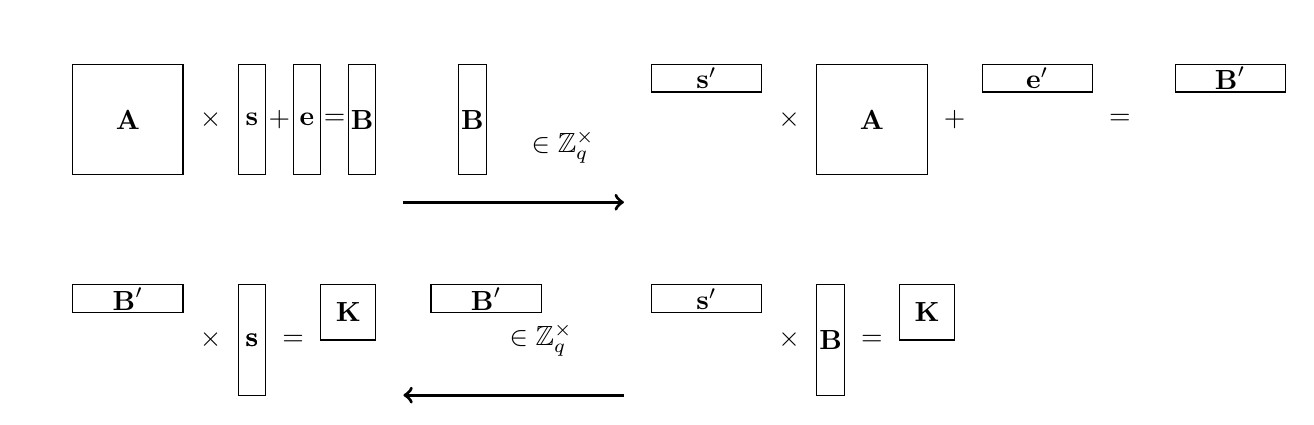
\begin{tikzpicture}[scale=0.7]

\node at (-0.65,5) {\dimension};\draw (0,4) rectangle (2,6);\node at (1,5) {$\textbf{A}$};\node at (1,6.5) {\dimension};
\node at (2.5,5) {$\times$};
\node at (3.25,6.5) {\error};\draw (3,4) rectangle (3.5,6);\node at (3.25,5) {$\textbf{s}$};
\node at (3.75,5) {$+$};

\node at (4.25,6.5) {\error};\draw (4,4) rectangle (4.5,6);\node at (4.25,5) {$\textbf{e}$};
\node at (4.75,5) {$=$};
\node at (5.25,6.5) {\error};\draw (5,4) rectangle (5.5,6);\node at (5.25,5) {$\textbf{B}$};

\draw[very thick,->] (6, 3.5) -- (10, 3.5);\draw (7,4) rectangle (7.5,6);\node at (7.25,5) {$\textbf{B}$};\node at (8.9,4.5) {$\in \mathbb{Z}^{\dimension \times \error}_q$};

\node at (10, 5.75) {\error};\draw (10.5,5.5) rectangle (12.5,6);\node at (11.5, 5.75) {$\textbf{s}'$};\node at (11.5, 6.5) {\dimension};
\node at (13, 5) {$\times$};
\node at (14.5, 6.5) {\dimension};\draw (13.5,4) rectangle (15.5,6);\node at (14.5, 5) {$\textbf{A}$};

\node at (16, 5) {$+$};
\draw (16.5,5.5) rectangle (18.5,6);\node at (17.5, 5.75) {$\textbf{e}'$};\node at (17.5, 6.5) {\dimension};
\node at (19, 5) {$=$};
\node at (19.5, 5.75) {\error};\draw (20,5.5) rectangle (22,6);\node at (21, 5.75) {$\textbf{B}'$};\node at (21, 6.5) {\dimension};

\draw[very thick,<-] (6, 0) -- (10, 0);\draw (6.5,1.5) rectangle (8.5,2);\node at (7.5,1.75) {$\textbf{B}'$};\node at (8.5,1) {$\in \mathbb{Z}^{\error \times \dimension}_q$};

\node at (-0.5,1.75) {\error};\draw (0,2) rectangle (2,1.5);\node at (1,2.5) {\dimension};\node at (1,1.75) {$\textbf{B}'$};
\node at (2.5,1) {$\times$};
\node at (3.25,2.5) {\error};\draw (3,0) rectangle (3.5,2);\node at (3.25,1) {$\textbf{s}$};
\node at (4,1) {$=$};
\node at (5,2.5) {\error};\draw (4.5,2) rectangle (5.5,1);\node at (4.10,1.5) {\error};\node at (5,1.5) {$\textbf{K}$};


\node at (10,1.75) {\error};\draw (10.5,1.5) rectangle (12.5,2);\node at (11.5, 1.75) {$\textbf{s}'$};\node at (11.5, 2.5) {\dimension};
\node at (13, 1) {$\times$};
\draw (13.5,0) rectangle (14,2);\node at (3.25,1) {$\textbf{s}$};\node at (13.75,2.5) {\error};\node at (13.75,1) {$\textbf{B}$};
\node at (14.5,1) {$=$};
\node at (15.5,2.5) {\error};\draw (15,2) rectangle (16,1);\node at (14.6,1.5) {\error};\node at (15.5,1.5) {$\textbf{K}$};

\end{tikzpicture}
\end{center}
\caption{Visualization of $\mathrm{LWE}$ based key-exchange}
Resulting shared key is a $\error \times \error$ matrix
\end{figure}


The first issue that emerges is matrix inversion, multiplication are both costly in terms of both space and time. Another important issue is sharing a matrix $\textbf{A}$ is costly with regards to the bandwidth needed for key-exchange. Moreover, to achieve a reasonable security we need at least $1024 \times 1024$ matrix to be shared.

\begin{figure}[H]
\centering
	$\begin{bmatrix} 
		4  & 1  & 11 & 10 \\
		5 & 5 & 9 & 5 \\
		3 & 9 & 8 & 10  \\
		1  & 3 & 3 & 2 
	\end{bmatrix}$
	vs.
    $\underbrace{
    \begin{rcases}
    \begin{bmatrix} 
		2738 & 3842 & 3345 & 2979 & \dots\\
		2896 & 595 & 3607 & \dots \\
		377 & 1575  & \dots \\
        2760 & \dots \\
        \dots
	\end{bmatrix}
    \end{rcases}}_\text{1024 rows}\text{1024 columns}$
	\caption{Toy example $\mathbb{Z}_{13}^{4\times4}$ vs. real-world example $\mathbb{Z}_{4093}^{1024\times1024}$ of random shared matrix}
	{The example on the right is modulo $4093$ so each matrix element in the field of $\mathrm{Z}_{4093}^{1024 \times 1024}$ would require at most $12$ bits. Therefore, $12 \times 1024 \times 1024 = 4291821568 \text{ bits} \approx 1.5 \text{ Megabyte}$}.
\end{figure}

Hence, to overcome above issues we can use cyclic matrices to give matrix some structure and ultimately reduce the size.

\begin{plain}
\normalfont
Circulant matrices (cyclic matrix) form a commutative ring, since for any two given circulant matrices $\textbf{A}$ and $\textbf{B}$, the sum $\textbf{A}+\textbf{B}$ is circulant, the product $\textbf{A} \times \textbf{B}$ is circulant, and $\textbf{A} \times \textbf{B}=\textbf{B} \times \textbf{A}$
\end{plain}

\begin{plain}
\normalfont
A polynomial in a ring $\mathbb{Z}[x] / (x^n-1)$ can be represented as a $n \times n$ circulant matrix. That is:

\[a_0 + a_1x + \dots + a_{n-1}x^{n-1} \mapsto \begin{bmatrix}a_0&a_1 &\dots& a_{n-1} \\a_{n-1}&a_0 &\dots & a_{n-2} \\\dots&\dots&\dots&\dots \\a_{1} & a_2 &\dots& a_0\end{bmatrix}\]
\end{plain}

To solve bandwidth problem, by using cyclic matrix instead then matrix calculation would get a cumulative property for free, so no need to shuffle and transpose matrices as demonstrated previously. As a result, we do not need to send the complete matrix to other party, we can just send the first row and the other party can re-create the matrix. Using polynomials instead of matrix would address the high cost of matrix multiplication and inversion. As noted above, polynomial in $\mathbb{Z}[x] / (x^n - 1)$ can be represented as a cyclic matrix. But as noted before, conjecture is $\mathrm{SVP}_{poly(n)}$ for ideals in $\mathbb{Z}[x]/(f)$ takes time $2^{\Omega(n)}$ when $f$ is irreducible polynomial (if $f$ is not irreducible then multiplication operation would not be invertible in general, and hence we would not get a field and subsequently lattice would not be ideal).


% \begin{figure}[H]
% \centering
% 	$
% 	\begin{bmatrix} 
% 		4  & 1  & 11 & 10 \\
% 		10 & 4  & 1  & 11 \\
% 		11 & 10 & 4  & 1  \\
% 		1  & 11 & 10 & 4  \\
% 		4  & 1  & 11 & 10
% 	\end{bmatrix}
% 	\to
% 	\begin{bmatrix} 
%         4  & 1  & 11 & 10 \\
% 	    3  & 4  & 1  & 11 \\
% 	    2  & 3  & 4  & 1  \\
% 	    12 & 2  & 3  & 4  \\
% 	    9  & 12 & 2  & 3  \\
% 	    10 & 9  & 12 & 2  \\
% 	    11 & 10 & 9  & 12 \\
% 	    1  & 11 & 10 & 9  \\
% 	    4  & 1  & 11 & 10
% 	\end{bmatrix}$
% 	\caption{Demonstration of cyclic matrix in $\mathrm{LWE}$ (toy example)}
% 	\footnotesize{Note that we do not need to sent the complete matrix, sending the first row is enough to re-create the matrix.	Also, after first $4$ rows on the left and $2 \times 4 = 8$ rows on the right, rows are repeating so no new vector is introduced after those rows.}
% \end{figure}

Simple irreducible polynomial can be: $x^n + 1$. We can use a wrapping rule to represent a polynomial in $\mathbb{Z}[x] / (x^n + 1)$ when $n$ is a power of $2$. This would remove any pattern in cyclic matrix and subsequently makes it more complex. The wrapping rule can be: ${x \mapsto -x \bmod \ 13}$ applied to the shifted value. In other words, do a circular right shift to every row and apply above map to the value of first column of shifted row.


Below shows that by treating the first row of cyclic matrix as a polynomial in quotient polynomial ring over finite field of $\mathbb{Z}_{13}[x] / ( x^{4} + 1 )$, polynomial can be represented as a wrapping rule described above (i.e. $\mathbb{Z}^{4 \times 4}_{13}$). In details, we can construct the same matrix using the first row of matrix as a polynomial in quotient ring over finite field and then multiplying it by $x^i$ for $0 \le i < n$ to re-create original matrix.


\begin{figure}[H]
\centering
    $\begin{bmatrix} 
            4& 1& 11& 10\\
    	    3& 4& 1& 11\\
    	    2& 3& 4& 1\\
    	    12& 2& 3& 4
    \end{bmatrix}
    \leftrightarrow
    \begin{matrix} 
            x^0 \times (4x^0+ 1x^1+ 11x^2+ 10x^3) = 4x^0+ 1x^1+ 11x^2+ 10x^3 \to [4, 1, 11, 10]\\
    	    x^1 \times (4x^0+ 1x^1+ 11x^2+ 10x^3) = 3x^0+ 4x^1+ 1x^2+ 11x^3  \to [3, 4, 1, 11]\\
    	    x^2 \times (4x^0+ 1x^1+ 11x^2+ 10x^3) = 2x^0+ 3x^1+ 4x^2+ 1x^3 \to [2, 3, 4, 1]\\
    	    x^3 \times (4x^0+ 1x^1+ 11x^2+ 10x^3) = 12x^0+ 2x^1+ 3x^2+ 4x^3 \to [12, 2, 3, 4]\\
     \end{matrix}$
     \caption{Demonstration of simple wrapping rule to create cyclic matrix in Ring-$\mathrm{LWE}$}
     It is essentially multiplying the first row with $x^i$ for $i \in [0, n-1]$ and extract coefficients.
\end{figure}



The above wrapping rules helps to visualize Ring variant of LWE where irreducible polynomial is $x^n + 1$, in terms of a matrix. But polynomial multiplication is substantially more efficient in terms of both space and time. So by using Ring variant of LWE (i.e. treating $A, s, e$ as polynomials instead of matrices), we can make key-exchange process substantially more efficient. 


\iftoggle{verylong}{
\lstinputlisting[language=Python, caption=Implementation of wrapping rule and testing if it equals to Quotient ring in SageMath]{code_snippets/cyclic_matrix_rlwe.sage}
}{}



\subsection{Reason to use a reconciliation method}
Below is a Diffie-Hellman like key-exchange in Ring-$\mathrm{LWE}$. Note that $A$ is a shared polynomial, $s$ is a secret polynomial and $e$ is a noise polynomial. Only polynomials $A$ and $b$ are shared between two parties and $s, e$ are both kept secret. 

\begin{figure}[H]
    \centering
	Alice chooses {small} $s$, $e$ in ${\mathbb{Z}}_{q}$, both sampled from a noise distribution\\
	Bob chooses {small} $s'$, $e'$ in ${\mathbb{Z}}_{q}$, both sampled from a noise distribution\\
	Alice $\to$ Bob: $b = A \times s + e$\\
	Bob $\to$ Alice: $b' = A \times s' + e'$\\
	Shared secret Alice calculates: $s \times b' = s \times (A \times s' + e') = A \times s   \times s' + \boldsymbol{s \times e'}$\\
	Shared secret Bob calculates: $s' \times b = s' \times (A \times s + e) = A \times s   \times s' + \boldsymbol{s' \times e}$
	\caption{Basic Ring-$\mathrm{LWE\text{-}DH}$ key agreement}
	{$A$ is similar to generator ($g$) and $q$ (prime) is similar to modulo prime in Diffie-Hellman key exchange}
\end{figure}

Notice that shared keys do not match because ${s} \times {e}' \neq {s}' \times {e}$. Although errors are supposed be relatively small compared to shared polynomial ${A}$ and their product with secret would be small as a result (i.e. $||{s} \times {e}'|| , ||{s}' \times {e}|| \ll ||A||$), but still resulting shared key do not match and it is a problem if one wants to construct a cryptographic key-exchange protocol. To overcome this issue we use rounding methods to extract a bit from every coefficient and as added error is relatively small, hence, the coefficients would not differ significantly. Therefore, rounding method eliminates the error and extracts the same shared key for both parties. There are two types of rounding methods (or reconciliation techniques): 

\begin{enumerate}
    \item reconciliation without any rounding information (e.g. Regev's basic rounding method)
    \item reconciliation with rounding information to substantially increase the probability of extracting the same key.
\end{enumerate}

The idea of sending extra bits was initially introduced by Ding and later improved by Peikert and Alkim et al.

\begin{lemma}
    \normalfont
    (\cite{DBLP:conf/crypto/ApplebaumCPS09}, Lemma 2)
    $\mathrm{LWE}$ is no easier if the secret is drawn from the error distribution $\chi^{n}$
    % This is also called the \text{Hermite normal form} of $\mathrm{LWE}$ \cite{Micciancio2009}.
\end{lemma}

The advantage to sample $\textbf{s}$ and $\textbf{e}$ from normal distribution (Gaussian) is the guarantee that $\langle \textbf{s}, \textbf{e} \rangle$ is small. Hence, during decryption, terms that look like $\langle \textbf{s}, \textbf{e} \rangle$ (inner product of the secret vector $\textbf{s}$ and error vector $\textbf{e}$) appears in the decryption. In Ring variant of key-exchange, we receive as shared key ${s} \times ({A} {s}'+{e}')={A} {s}{s}'+{s}{e}' \leftrightarrow {s}' \times ({A} {s}+{e})={A} {s} {s}'+{s}' {e}$. So if both parties choose small $s$ and $s'$ (hence their inner product with error terms would be small) and then chance of reconciliation failing to extract the same key would be reduced substantially. 


% \begin{plain}
%     \normalfont
% There is an advantage to sample $s$ and $e$ from normal distribution (Gaussian):
% \begin{itemize}
%     % \item Guarantees that $\textbf{s}$ and $\textbf{e}$ have large norms (Euclidean norm)
%     \item Guarantees that $\langle s, e \rangle$ is small
%     \item Gaussian distribution has relatively high entropy in comparison with uniform distribution (discrete uniform sampler from $[0,  \sigma)$) and achieves the above properties
% \end{itemize}
% \end{plain}

% \begin{definition}
% \normalfont
% Given a basis $\textbf{B} =\{\mathbf{b} _{1},\mathbf {b} _{2},\dots ,\mathbf {b}_{d}\}$ with $n$-dimensional integer coordinates, for a lattice $\mathcal{L}$ (a discrete subgroup of $\mathbb{R}^n$) with $d\leq n$, the $\mathrm{LLL}$ algorithm calculates an $\mathrm{LLL}$-reduced (short, nearly orthogonal) lattice basis in time $\mathcal{O}(d^{5}n\log ^{3}B)$, where .
% \end{definition}

% The $l_{2}$ norm is important in cryptanalysis. When an attacker is trying to recover the secret key or the message, he will set up a lattice and try to find a short vector. We know how to judge the running time of lattice-reduction algorithms based on the $l_{2}$ norm of the vector they are trying to find. In particular, $\mathrm{LLL}$ (and its variants) are analyzed in terms of the $l_{2}$ norm (i.e. time complexity of $\mathrm{LLL}$ is $\mathcal{O}(d^{5}n\log ^{3}B)$ where $B$ is the largest length of $b_{i}$ under the Euclidean norm $l_{2}$).


\section{Reconciliation methods}
Below is a description of different reconciliation methods in Ring-$\mathrm{LWE}$. These methods apply to every coefficient of resulting shared key which is a polynomial in Ring-$\mathrm{LWE}$. These methods can also be applied to $\mathrm{LWE}$ based key-exchange as well by applying them to respective matrix elements.


\subsection{Rounding method in Ring-\texorpdfstring{$\mathrm{LWE}$}{LWE} suggested by Regev}
As each coefficient of polynomial is an integer modulo $q$, then we can round each coefficient to either to $0$ or $1$. Regev's suggested to round every coefficient if it in $( \frac{-q}{2}, \frac{-q}{4}] \cup (\frac{q}{4}, \frac{q}{2}]$ to $1$, and round if it is in $(\frac{-q}{ 4}, \frac{q}{4}]$ to $0$. This basic method works most of the time and probability of failure is $\frac{1}{2^{10}}$ which is not good enough considering that we have $1024$ coefficients in our shared polynomial to achieve a reasonable security.



\begin{figure}[H]
	\centering
	\begin{tabular}{|lll|}
		\hline
		\textbf{Alice}                                       &                               & \textbf{Bob}                               \\\hline
		$s, e \gets \chi$, $A \gets \text{uniformly random}$ &                               & $s', e' \gets  \chi$                       \\
		                                                     & $\xrightarrow{ A, b = As + e}$ &                                            \\
		                                                     & $\xleftarrow{b' = As' + e'}$  &                                            \\
				 		
		$K = \texttt{reconcile}(s \times b')$          &                               & $K = \texttt{reconcile}(s' \times b)$ \\\hline
	\end{tabular}
	\caption{Diagram of basic Diffie-Hellman like key-exchange protocol in Ring-$\mathrm{LWE}$}
    \figuresubtitle{Note that $s, e$ and $s', e'$ are all sampled from a noise distribution but $A$ is generated uniformly at random. Also, \texttt{reconcile} function applies Regev's basic rounding method to every coefficient of resulting polynomial.}
\end{figure}

\begin{figure}[H]
	\begin{center}
		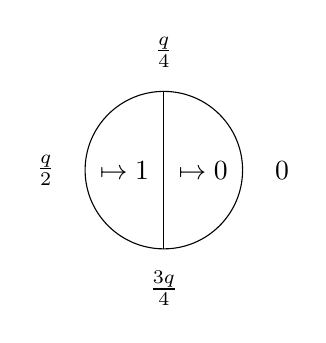
\begin{tikzpicture}
			\draw (2,2) circle (1cm);
			\draw (2,2) -- (2,3);
			\draw (2,2) -- (2,1);
											
			\node at (3.5,2) {$0$};
			\node at (2,3.5) {$\frac{q}{4}$};
			\node at (0.5,2) {$\frac{q}{2}$};
			\node at (2,0.5) {$\frac{3q}{4}$};
											
			\node at (2.5,2) {$\mapsto 0$};
			\node at (1.5,2) {$\mapsto 1$};
											
		\end{tikzpicture}
	
	Alice's calculated shared key:
	    
	$4079331x^0 + 1894732x^1 + \dots + 472608x^{1022} + 516748x^{1023} = 01 \dots 00$
	\\~\\ 
	Bob's calculated shared key:
	    
	$4079332x^0 + 1894733x^1 + \dots + 472607x^{1022} + 516748x^{1023} = 01 \dots 00$
	\caption{Demonstration of Regev's rounding approach}
	\figuresubtitle{Notice coefficients of both parties are close but not equal. In Regev's rounding approach, we round each efficient to either $0$ or $1$ based on the region coefficient is located at.}
    \end{center}
\end{figure}



\subsection{Improved rounding method as suggested by Ding}
Regev's method can be modified slightly by multiplying error terms by $2$. The goal is to make sure difference between error terms would be even. Thereafter, we would follow the naive approach of $\bmod 2$ to eliminate the terms $2 \times s \times e'$ and $2 \times s' \times e$, hence, resulting shared key would match. However this would not result in any improvement because difference between calculated key of both parties would not always be even, since we are working in $\mathbb{Z}_{q}$ as oppose to $\mathbb{Z}$ and $q$ is an odd prime. Therefore, further adjustments are needed.


\begin{figure}[H]
    \centering
	Alice chooses {small} $s$, $e$ in ${\mathbb{Z}}_{q}$, both sampled from a noise distribution\\
	Bob chooses {small} $s'$, $e'$ in ${\mathbb{Z}}_{q}$, both sampled from a noise distribution\\
	Alice $\to$ Bob: $b = A \times s + 2 \times e$\\
	Bob $\to$ Alice: $b' = A \times s' + 2 \times e'$\\
	Shared secret Alice calculates: $s \times b' = s \times (A \times s' + 2 \times e') = A \times s   \times s' + 2\times s \times e'$\\
	Shared secret Bob calculates: $s' \times b = s' \times (A \times s + 2 \times e) = A \times s   \times s' + 2 \times s' \times e$
	$A \times s   \times s' + 2\times s \times e' - A \times s   \times s' + 2 \times s' \times e = 2 \times (s\times e' - s' \times e)\leftarrow \textbf{not necessarily even difference}$
	\caption{Demonstration of using even error values in basic Ring-$\mathrm{LWE\text{-}DH}$ key agreement}
	\figuresubtitle{For example, in $\mathbb{Z}$, $2 \times 7 = 14$ which is an even number but in $\mathbb{Z}_{13}$, it would be $1$ which is an odd number.}
\end{figure}


\begin{figure}[H]
    \centering
	\begin{center}
    \begin{tikzpicture}[scale=0.95]
			\draw (2,2) circle (1cm);
			\draw (2,2) -- (2,3);
			\draw (2,2) -- (2,1);
											
			\node at (3.5,2) {$0$};
			\node at (2,3.5) {$\frac{q}{4}$};
			\node at (0.5,2) {$\frac{q}{2}$};
			\node at (2,0.5) {$\frac{3q}{4}$};
											
			\node at (2.5,2) {$\mapsto 0$};
			\node at (1.5,2) {$\mapsto 1$};

    		\fill (2.3,2.95)  circle[radius=2pt];
    		\fill (1.7,2.95)  circle[radius=2pt];
		
            \draw[-stealth] (-3,-1)--(6,-1);
            \node at (7, -1){x};
            \node at (7, 0) {$\mathbb{Z}$};
            \draw (-2, -1)  circle[radius=2pt];\node at (-2, -1.5) {-2};			
            \draw (-1, -1)  circle[radius=2pt];\node at (-1, -1.5) {-1};
            \draw (0, -1)  circle[radius=2pt];\node at (0, -1.5) {0};
            \draw (1, -1)  circle[radius=2pt];\node at (1, -1.5) {1};
            \draw (2, -1)  circle[radius=2pt];\node at (2, -1.5) {2};
            \draw (3, -1)  circle[radius=2pt];\node at (3, -1.5) {3};
            \draw (4, -1)  circle[radius=2pt];\node at (4, -1.5) {4};
            \draw (5, -1)  circle[radius=2pt];\node at (5, -1.5) {5};
            
            \fill (2,-1)  circle[radius=4pt];
            \fill (4,-1)  circle[radius=4pt];
            \draw[thick,|<->|] (2, -0.5) -- (4, -0.5); 	
            \draw (2, -1) -- (2, 0); 	
            \draw (4, -1) -- (4, 0); 
            
            \draw[-stealth] (-3,-4)--(6,-4);
            \node at (7, -4){x};
            \node at (7,-3) {$\mathbb{Z}_{q}$ (e.g. $\mathbb{Z}_{5} \in \{-2, -1, 0, 1, 2\}$)};
            \draw (-2, -4)  circle[radius=2pt];\node at (-2, -4.5) {-2};			
            \draw (-1, -4)  circle[radius=2pt];\node at (-1, -4.5) {-1};
            \draw (0, -4)  circle[radius=2pt];\node at (0, -4.5) {0};
            \draw (1, -4)  circle[radius=2pt];\node at (1, -4.5) {1};
            \draw (2, -4)  circle[radius=2pt];\node at (2, -4.5) {2};
            \draw (3, -4)  circle[radius=2pt];\node at (3, -4.5) {3};
            \draw (4, -4)  circle[radius=2pt];\node at (4, -4.5) {4};
            \draw (5, -4)  circle[radius=2pt];\node at (5, -4.5) {5};
            
            \fill (2,-4)  circle[radius=4pt];
            \fill (-1,-4)  circle[radius=4pt];
            \draw[thick,|<->|] (2, -3.5) -- (-1, -3.5); 	
            \draw (2, -4) -- (2, -3); 	
            \draw (-1, -4) -- (-1, -3); 
		\end{tikzpicture}
		\end{center}
		\caption{Demonstration of only multiplying errors by $2$ will not help the reconciliation}
		\figuresubtitle{In $\mathbb{Z}$ difference between two points is even but in $\mathbb{Z}_{5}$ difference is odd, hence no benefit in just multiplying error terms by $2$. More than just multiplying error terms by $2$ is needed.}
\end{figure}




Ding in \cite{ding2012simple} proposed a reconciliation method based on Ring-$\mathrm{LWE}$. This protocol is the first to introduce the idea of sending extra information to improve success rate of reconciliation. Peikert improved Ding's method in \cite{peikert2014lattice} and presented a $\mathrm{KEM}$ (key-exchange mechanism). Later on Peikert's $\mathrm{KEM}$ was used in the construction of the $\mathrm{BCNS}$ protocol \cite{bos2015post} which itself was recently improved, resulting in the $\mathrm{NewHope}$ protocol by Alkim et al. \cite{alkim2015post}.

The basic idea of Ding's method can be seen as Diffie-Hellman like key exchange protocol based on the Ring-$\mathrm{LWE}$ problem. The key-exchange protocol is secure against passive adversaries if Ring-$\mathrm{LWE}$ is hard. For a proof and an exact definition of this security model we refer to \cite{ding2012simple}. The key exchange protocol is only proven to be secure in the two-user setting. A multi-user variant is proposed in the same paper, but its security is not yet proven. To describe Ding's reconciliation method, we define the following functions: $\delta: \mathbb{Z}_{q} \mapsto \{0, 1\}$, $Signal: \mathbb{Z}_{q} \mapsto \{0, 1\}$, and $Encode: \mathbb{Z}_{q} \times \{0, 1\} \mapsto \{0, 1\}$ via:

\begin{equation}
Signal(x) = \delta(x) \mapsto
\begin{cases*}
  0 & if $x \in [-\lfloor \frac{q}{4} \rfloor$, $\lfloor\frac{q}{4} \rceil]$\\
  1 & otherwise
\end{cases*}
\end{equation}

% \begin{equation}
% \delta_{1}(x) =
% \begin{cases*}
%   0 & if $x \in [-\lfloor \frac{q}{4}\rfloor +1$, $\lfloor\frac{q}{4}\rfloor +1]$\\
%   1 & otherwise
% \end{cases*}
% \end{equation}

% \begin{equation}
% Signal(x) = \delta(x)
% \end{equation}

\begin{equation}
Encode(x, \delta) = (x + \delta \times (\frac{q-1}{2}) \bmod q) (\bmod 2)
\end{equation}





The basis idea is that if coefficient is in inner region ($\delta = 0$) , then we just $\bmod 2$ because the difference between $2 \times s \times e'$ and $2 \times s'\times e$ is even with high probability, hence in inner region the probability of achieving the same $\bmod 2$ of coefficient is much higher than outer region. What we want to avoid while $\bmod 2$ is coefficient of two parties are in different regions. So, if signal bit is in outer region ($\delta = 1$), then we add $\frac{q-1}{2}$ to respective coefficient. Therefore, coefficient will now be in inner region and then $\bmod 2$.



\begin{figure}[H]
    \centering
	\begin{center}
    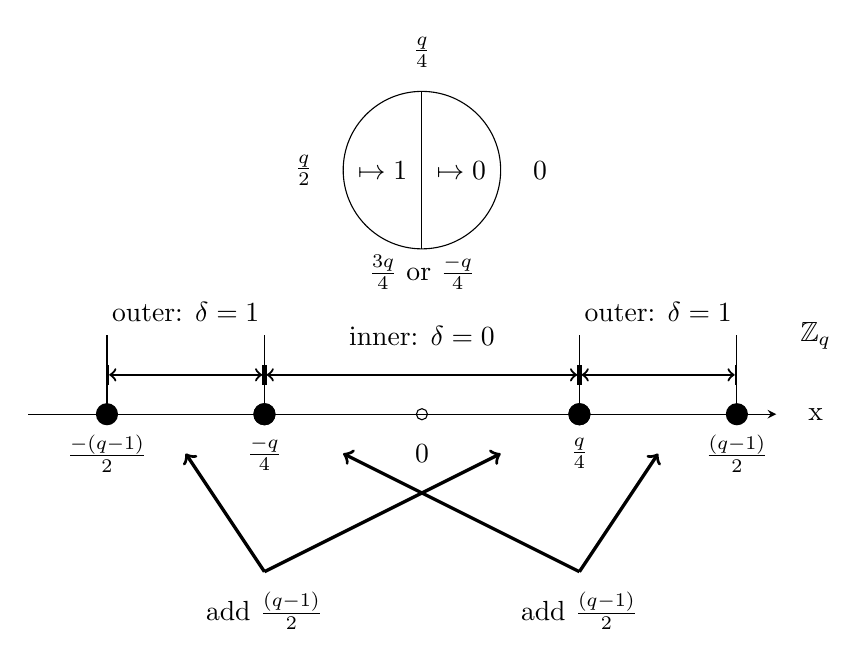
\begin{tikzpicture}
			\draw (2,2.1) circle (1cm);
			\draw (2,2.1) -- (2,3.1);
			\draw (2,2.1) -- (2,1.1);
											
			\node at (3.5,2.1) {$0$};
			\node at (2,3.6) {$\frac{q}{4}$};
			\node at (0.5,2.1) {$\frac{q}{2}$};
			\node at (2,0.8) {$\frac{3q}{4}$ or $\frac{-q}{4}$};
											
			\node at (2.5,2.1) {$\mapsto 0$};
			\node at (1.5,2.1) {$\mapsto 1$};


            \draw[-stealth] (-3,-1)--(6.5,-1);
            \node at (7, -1){x};
            \node at (7, 0) {$\mathbb{Z}_{q}$};
            \draw (-2, -1)  circle[radius=2pt];\node at (-2, -1.5) {$\frac{-(q-1)}{2}$};			
            \draw (0, -1)  circle[radius=2pt];\node at (0, -1.5) {$\frac{-q}{4}$};			
            \draw (2, -1)  circle[radius=2pt];\node at (2, -1.5) {$0$};	
            \draw (4, -1)  circle[radius=2pt];\node at (4, -1.5) {$\frac{q}{4}$};			
            \draw (6, -1)  circle[radius=2pt];\node at (6, -1.5) {$\frac{(q-1)}{2}$};			

            \fill (6,-1)  circle[radius=4pt];
            \fill (4,-1)  circle[radius=4pt];
            \draw[thick,|<->|] (4, -0.5) -- (6, -0.5); 	
            \draw (4, -1) -- (4, 0); 	
            \draw (6, -1) -- (6, 0); 
  			\node at (5,0.3) {outer: $\delta = 1$};

            \fill (-2,-1)  circle[radius=4pt];
            \fill (0,-1)  circle[radius=4pt];
            \draw[thick,|<->|] (-2, -0.5) -- (0, -0.5); 	
            \draw (-2, -1) -- (-2, 0); 	
            \draw (0, -1) -- (0, 0); 
  			\node at (2,0) {inner: $\delta = 0$};

            \fill (0,-1)  circle[radius=4pt];
            \fill (4,-1)  circle[radius=4pt];
            \draw[thick,|<->|] (0, -0.5) -- (4, -0.5); 	
            \draw (4, -1) -- (4, 0); 	
            \draw (6, -1) -- (6, 0); 
  			\node at (-1,0.3) {outer: $\delta = 1$};

    		\draw[very thick,<-] (-1,-1.5) -- (0,-3);
    		\draw[very thick,<-] (3,-1.5) -- (0,-3);
    		\node at (0, -3.5){add $\frac{(q-1)}{2}$};
    
    		\draw[very thick,<-] (1,-1.5) -- (4,-3);
    		\draw[very thick,<-] (5,-1.5) -- (4,-3);
            \node at (4, -3.5){add $\frac{(q-1)}{2}$};
    

		\end{tikzpicture}
		\end{center}
		\caption{Demonstration of signal function in $\mathrm{DXL}$ protocol}
		\figuresubtitle{If $\delta = 1$ or we are in outer region, then we add $\frac{q-1}{2}$ to respective coefficient, hence we will be in inner region and then $\bmod 2$; if $\delta = 0$ then we just $\bmod 2$.}
\end{figure}



% \subsection*{\texorpdfstring{$\mathrm{DXL}$}{DXL} Protocol construction}
Ding in the same paper introduced $\mathrm{DXL}$ key-exchange protocol. However, this protocol never got implemented in an efficient manner but it had an impact on future key-exchange protocols. For example, adding secondary noise to the calculated polynomial key to prevent secret leakage and increase entropy (additive noise).

The key exchange in this protocol will take place between two parties. There will be an initiator for the key exchange designated as ($I$) and a respondent designated as ($R$). Both $I$ and $R$ know $q$, $n$, $a(x)$, and have the ability to generate small polynomials according to the distribution $\chi_{\sigma}$ with parameter $\sigma$. The distribution $\chi_{\sigma}$ is a discrete Gaussian distribution. The key-exchange begins with the initiator ($I$) doing the following:

\noindent\textbf{Initiation}
\begin{enumerate}
    \item Generate two polynomials $s_{I}$ and $e_{I}$ with small coefficients by sampling from the distribution $\chi _{\sigma }$.
    \item Compute $p_{I}=as_{I}+2e_{I}$.
    \item The initiator sends the polynomial $p_{I}$ to the Responder.
\end{enumerate}

\noindent\textbf{Response}
\begin{enumerate}
    \item Generate two polynomials $s_{R}$ and $e_{R}$ with small coefficients by sampling from the distribution $\chi _{\sigma }$
    \item Compute $p_{R}=as_{R}+2e_{R}$
    \item Generate a small $e'_{R}$ from $\chi _{\sigma }$. Compute $k_{R}=p_{I}s_{R}+2e'_{R}$. Then $k_{R}=as_{I}s_{R}+2e_{I}s_{R}+2e'_{R}$
    \item Use the signal function $Signal$ to find $w=Signal(k_{R})$. This is computed by applying $Signal$ function on each coefficient of $k_{R}$
    \item Respondent side's key stream $sk_{R}=Encode(k_{R}, w)$ is calculated, based on the reconciliation information $w$ and the polynomial $k_{R}$
    \item The Respondent sends $p_{R}$ and $w$ to the Initiator
\end{enumerate}

\noindent\textbf{Finish}
\begin{enumerate}
    \item Receive $p_{R}$ and $w$ from the Responder
    \item Sample $e'_{I}$ from $\chi _{\sigma }$ and Compute $k_{I}=p_{R}s_{I}+2e'_{I}=as_{I}s_{R}+2e_{R}s_{I}+2e'_{I}$
    \setcounter{enumi}{0}
    \item Initiator side's key stream is produced as $sk_{I}=Encode(k_{I}, w)$ from the reconciliation information $w$ and polynomial $k_I$
\end{enumerate}









\subsection{Rounding method as utilized in $\mathrm{BCNS}$ protocol}
In 2014, Peikert in \cite{peikert2014lattice} presented a key transport scheme following the same basic idea of Ding's, where the idea of sending additional $1$ bit signal for every coefficient is also utilized. In this improved approach, Bob sends Alice a reconciliation information $\in \{0,1\}^n$ (similar to output of signal function in Ding's method) such that $0 \mapsto region\ \#1$, $1 \mapsto region\ \#2$. In other words, as a reconciliation information one party sends a region number that his or her coefficient is located in. Then based on the region, a particular key extraction rule applies. If $v, u$ are respective coefficients of Alice and Bob, and also $|u-v| \le \frac{q}{8}$, then this method always works. Due to the clever design of rounding regions and key extractions rules, revealing the region leaks no information and does not compromises security.

We should note that $\mathrm{BCNS}$ protocol is an implementation of Peikert's reconciliation method and this protocol does not introduce a new reconciliation method.

\begin{figure}[H]
	\centering
	\begin{subfigure}[t]{0.3\textwidth}
		\centering
		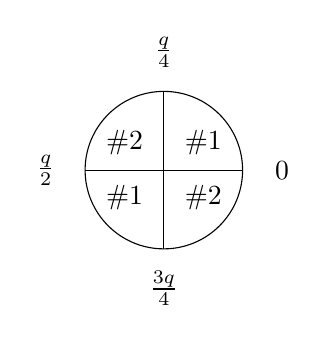
\begin{tikzpicture}
			\draw (2,2) circle (1cm);
			\draw (2,2) -- (2,3);
			\draw (2,2) -- (2,1);
			\draw (2,2) -- (3,2);
			\draw (2,2) -- (1,2);
											
			\node at (3.5,2) {$0$};
			\node at (2,3.5) {$\frac{q}{4}$};
			\node at (0.5,2) {$\frac{q}{2}$};
			\node at (2,0.5) {$\frac{3q}{4}$};
													
			\node at (2.5,2.35) {\#1};
			\node at (2.5,1.65) {\#2};
									
			\node at (1.5,2.35) {\#2};
			\node at (1.5,1.65) {\#1};
		\end{tikzpicture}
		\caption{4 rounding regions}
	\end{subfigure}
	\hfill
	\begin{subfigure}[t]{0.3\textwidth}
		\centering
		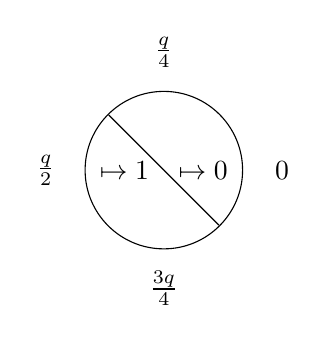
\begin{tikzpicture}
			\draw (2,2) circle (1cm);
			\draw (2,2) -- (1.3,2.7);
			\draw (2,2) -- (2.7,1.3);
						
			\node at (3.5,2) {$0$};
			\node at (2,3.5) {$\frac{q}{4}$};
			\node at (0.5,2) {$\frac{q}{2}$};
			\node at (2,0.5) {$\frac{3q}{4}$};
									
			\node at (2.5,2) {$\mapsto 0$};
			\node at (1.5,2) {$\mapsto 1$};
		\end{tikzpicture}
		\caption{Case \#1}
	\end{subfigure}    
	\hfill
	\begin{subfigure}[t]{0.3\textwidth}
		\centering
		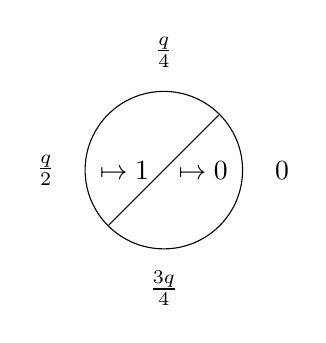
\begin{tikzpicture}
			\draw (2,2) circle (1cm);
			\draw (2,2) -- (2.7,2.7);
			\draw (2,2) -- (1.3,1.3);
						
			\node at (3.5,2) {$0$};
			\node at (2,3.5) {$\frac{q}{4}$};
			\node at (0.5,2) {$\frac{q}{2}$};
			\node at (2,0.5) {$\frac{3q}{4}$};
									
			\node at (2.5,2) {$\mapsto 0$};
			\node at (1.5,2) {$\mapsto 1$};
		\end{tikzpicture}
		\caption{Case \#2}
	\end{subfigure}
	\caption{Demonstration of Peikert's rounding approach}
	\figuresubtitle{(a) demonstrates the $4$ regions and (b) is a rounding rule when
	rounding information bit indicates regions \#1 and (c) if it indicates region \#2. Notice if difference of coefficients is $\le \frac{q}{8}$ then this method always works.}
\end{figure}		

% To improve polynomial multiplication speed, we can use $\mathrm{FFT}$ such that rather than working modulo degree-$1024$ polynomial with coefficients in ${\mathbb{Z}}_{q}$, we can work with degree-$256$ polynomial whose coefficients are themselves polynomials modulo a degree-$4$ polynomial. 
 

\begin{figure}[H]
    \centering
	Alice chooses \textit{small} $s$, $e$ in ${\mathbb{Z}}_{q}$, both sampled from a noise distribution\\
	Bob chooses \textit{small} $s'$, $e'$ in ${\mathbb{Z}}_{q}$, both sampled from a noise distribution\\
	Alice $\to$ Bob: $b = A \times s + e$\\
	Bob $\to$ Alice: $b' = A \times s' + e'$ and \textbf{rounding region} $ \in \{0,1\}^{n}$\\
	Shared secret Alice calculates: $s \times b' = s \times (A \times s' + e') = s \times A \times s' + s \times e'$\\
	Shared secret Bob calculates: $s' \times b = s' \times (A \times s + e) = s' \times A \times s + s' \times e$
	\caption{Exact Ring-$\mathrm{LWE\text{-}DH}$ key agreement as suggested by Peikert.}
	\figuresubtitle{Notice Bob also sends his rounding regions to Alice which is similar to Ding's rounding method}
\end{figure}		
		
% \subsubsection{\texorpdfstring{$\mathrm{KEM}$}{KEM} protocol description as suggested by Peikert}	

The following is the concrete description of Peikert's reconciliation method. We define the reconciliation mechanism where the modulus $q \ge 2$ is even, then define disjoint intervals $I_{0} = \{0, 1, \dots, \lfloor \frac{q}{4} \rceil- 1\}$, $I_{1} =  \{\lfloor \frac{3q}{4}\rceil, \dots, q-1\} \bmod q$. Now define the \textit{cross-rounding} function $\langle \cdot \rangle _{2}: \mathbb{Z}_{q} \to \mathbb{Z}_{2}$ as:


% $\langle v \rangle _{2}: = \lfloor \frac{4}{q} \cdot v \rfloor \bmod 2$. Equivalently, $\langle v \rangle_{2}$ is the $b \in \{0, 1\}$ such that $v$ belongs to the disjoint union $I_{b} \cup (\frac{q}{2} + I_{b})$.
 
% We see that these intervals form a partition of all the elements $v \in \mathbb{Z}_{q}$ such that $\lfloor v \rceil _{2} = 0$ (where we identify $0$ and $1$ with their residue classes modulo two). Similarly, $\frac{q}{2} + I_{0}$ and $\frac{q}{2} + I_{1}$ partition all the $v$ such that $\lfloor v \rceil _{2} = 1$.


% Let $q$ be an even modulus. Then we obtain:
% \[
% \lfloor v \rceil_{q, 2}  
% \begin{cases}
%     1 & v \in \{\lfloor \frac{q}{4} \rceil, \dots, \lfloor \frac{3q}{4} \rceil - 1 \} \\
%     0 &  v \in \{ 0, 1, \dots, \lfloor \frac{q}{4} \rceil - 1\} \cup \{ \lfloor \frac{3q}{4} \rceil, \dots, q - 1\}
% \end{cases}
% \]

% If $v$ is uniformly random, then $\langle v \rangle _{2}$ is uniformly random if and only if $\frac{q}{2}$ is even; otherwise, $\langle v \rangle_{2}$ is biased toward zero. Regardless of this potential bias, however, the theorem below shows that $\langle v \rangle_{2}$ hides $\lfloor v \rceil _{2}$ perfectly. 

% \begin{theorem}
%     \normalfont
%     For even $q$, if $v \in \mathbb{Z}_{q}$ is uniformly random, then $\lfloor v \rceil _{2}$ is uniformly random given $\langle v \rangle_{2}$.
% \end{theorem}

% \begin{theorem}
%     \normalfont
%     For even $q$, if $w = v + e \bmod q$ for some $v \in \mathbb{Z}_{q}$ and $e \in E$, then $\mathrm{rec}(w,\langle v \rangle_{2}) = \lfloor v \rceil _{2}$
% \end{theorem}

% The following is cross-rounding function:

\[
\langle v \rangle_{q, 2}=  
\begin{cases}
    0 & v \in I_{0} \cup (I_{0} + \frac{q}{2}) \\
    1 & v \in I_{1} \cup (I_{1} + \frac{q}{2})
\end{cases}
\]

% Let $I'_{1} = \{ \lfloor \frac{q}{2} \rfloor, \dots, -1\}$ and $I'_{0} = \{ 0, 1, \dots, \lfloor \frac{q}{2} \rceil -1 \}$. 

To compute the shared key the following reconciliation function $\text{rec}: \mathbb{Z}_{q} \times \mathbb{Z}_{2} \to \mathbb{Z}_{2}$ is used:

\[
\text{rec}(v, b) =
\begin{cases}
    0 & \text{if } v \in I_{b} + ([-\frac{q}{8}, \frac{q}{8}) \cap \mathbb{Z}) \bmod q\\
    % [-\frac{q}{2}, \frac{q}{2}) \\
    1 & \text{otherwise}
\end{cases}
\]


All of the above applies when $q$ is even, but in applications of Ring-$\mathrm{LWE}$ this is not the case. For instance, it is often desirable to let $q$ be a sufficiently large prime, for efficiency and security reasons. When $q$ is odd, while it is possible to use the above methods to agree on a bit derived by rounding a uniform $v \in \mathbb{Z}_{q}$, the bit will be biased, and hence not suitable as key material. Here we show how to avoid such bias by temporarily \textit{scaling up} to work modulo $2q$, and introducing a small amount of extra randomness.

Define the randomized function $\mathrm{dbl}: \mathbb{Z}_{q} \to \mathbb{Z}_{2q}$ that, given a $v \in \mathbb{Z}_{q}$, outputs $\bar{v} = 2v - \bar{e} \in \mathbb{Z}_{2q}$ for some random $\bar{e} \in \mathbb{Z}$ that is uniformly random modulo two and independent of $v$, and small in magnitude (e.g., bounded by one).


\[
\text{dbl}: \mathbb{Z}_q \to \mathbb{Z}_{2q}, x\mapsto2x - \bar{e}, \text{ where } \bar{e} = 
\begin{cases}
    -1 & \text{with probability } \frac{1}{4}\\
    0 & \text{with probability } \frac{1}{2}\\
    1 & \text{with probability } \frac{1}{4}\\
\end{cases}
\]


Moreover, if $w, v \in \mathbb{Z}_{q}$ are close, then so are $2w, \mathrm{dbl}(v) \in \mathbb{Z}_{2q}$, i.e., if $w = v+e (\bmod q)$ for some (small) $e$, thus $2e$ would be small too, then $2w = \bar{v} + (2e + \bar{e}) (\bmod 2q)$. Therefore, to (cross-) round from $\mathbb{Z}_{q}$ to $\mathbb{Z}_{2}$, we simply apply $\mathrm{dbl}$ to the argument and then apply the appropriate rounding function from $\mathbb{Z}_{2q}$ to $\mathbb{Z}_{2}$. Similarly, to reconcile some $w \in \mathbb{Z}_{q}$ we apply rec to $2w \in \mathbb{Z}_{2q}$; note that this process is still deterministic.

To summarize, The usual definition of (passive) security for key-exchange requires the agreed-upon key to be indistinguishable from uniformly random. That is not the case for 
$\mathrm{DXL}$ because the bits of the key are biased, not uniform. It is simply because any deterministic map from $\mathbb{Z}_{q}$ to $0,1$ must be biased when $q$ is odd. To address this issue, Peikert suggested if the modulus $q$ is odd, it requires to work in $\mathbb{Z}_{2q}$ instead of $\mathbb{Z}_{q}$ to avoid bias in the derived bits.


Since $q$ is odd in practice, we need use randomized doubling function (dbl). The following lemma shows that the rounding of $\mathrm{dbl}(v) \in \mathbb{Z}_{2q}$ for a uniform random element $v \in \mathbb{Z}_{q}$ is uniform random in $\mathbb{Z}_{2q}$ given its \textit{cross-rounding}.



\begin{lemma}
    \normalfont
    (\cite{peikert2014lattice}, Claim 3.3)
    For odd $q$, if $v \in \mathbb{Z}_{q}$ is uniformly random and $\bar{v} \leftarrow \mathrm{dbl}(v) \in \mathbb{Z}_{2q}$, then $\text{rec}(\bar{v})$ is uniformly random given $\langle \bar{v} \rangle_{2q, 2}$
\end{lemma}


% The first of these properties imply that if $v$ is uniformly random in $\mathbb{Z}_{q}$, then so is $\bar{v}$ in $\mathbb{Z}_{2q}$.

% \begin{lemma}
%     \normalfont
%     (\cite{peikert2014lattice}, Section 3.2)
%     For odd $q$, let $v=w+e\in \mathbb{Z}_q$ for $w,e\in \mathbb{Z}_q$ such that $2e\pm 1\in [-\frac{q}{4}, \frac{q}{4}) \pmod q$. Let $\bar v=\text{dbl}(v)$ then $\text{rec}(2w,\langle \bar v\rangle _{2q,2})=\lfloor \bar v \rceil _{2q,2}$
% \end{lemma}

\subsection{Rounding method as utilized in $\mathrm{NewHope}$ protocol}
In November 2015, Alkim, Ducas, Popplemann, and Schwabe in \cite{alkim2015post} built a reconciliation scheme based on the work of Peikert and further improved Peikert's randomized doubling function. In addition, Alkim et al. implemented their new reconciliation method as a protocol and named it $\mathrm{NewHope}$. Unlike $\mathrm{BCNS}$ protocol, $\mathrm{NewHope}$ protocol provides a new reconciliation methods and it is as follows: the sender and the receiver have two almost identical vectors $v_{S} \approx v_{R} \in \mathbb{Z}^{n}_{q}$. They want to obtain one shared secret key $SK \in \{0, 1\}^{\frac{n}{4}}$ from those two vectors, i.e., the sender and the receiver want to obtain one bit of the key from each four coordinates. Deciding the value of this key bit is done geometrically. In the following, by Voronoi cell we are referring to Polyhedron generated by Diamond cutting algorithm as described in \cite{481786} given full rank lattice with basis of $\begin{psmallmatrix}
    1   &   0   &   0   &   0\\
    0   &   1   &   0   &   0\\
    0   &   0   &   1   &   0\\
    0.5   &   0.5   &   0.5   &   0.5
\end{psmallmatrix}$, that is identity matrix such that last row is set to $\frac{1}{2}$.



\iftoggle{verylong}{
\lstinputlisting[language=Python, caption=Polyhedron generated by Diamond cutting algorithm]{code_snippets/voronoi_cell_plot.sage}
}{}


\begin{figure}[H]
\centering
\includegraphics[scale=0.3]{2-dimension-voronoi}
\caption{Voronoi cell in $2$-dimension}
\end{figure}


\begin{figure}[H]
\centering
\includegraphics[scale=0.35]{3-dimension-voronoi}
\caption{Voronoi cell in $3$-dimension}
\figuresubtitle{This is not being used in $\mathrm{NewHope}$, only for the purpose of visualization}
\end{figure}


\begin{figure}[H]
\centering
\includegraphics[scale=0.45]{4-dimension-voronoi}
\caption{Voronoi cell in $4$-dimension, (diamond inside a cube)}
\end{figure}


The essence of this new reconciliation can be summarized as the following:
\begin{enumerate}
    \item Divide every coefficient of calculated key, that is: $s' \times (As + e)$ or $s \times (As' + e')$ by $q$. Therefore we a get a list of numbers that are between $[0,1)$ inclusive
    \item Pairwise select every $4$ coefficient $(c_{i}, c_{i+1}, c_{i+2}, c_{i+3})$ and run the $p_{i} = \mathrm{CVP}_{4}(c_{i}, c_{i+1}, c_{i+2}, c_{i+3})$ to get the closest center of Voronoi cell, then store the result into array $[p_{1}, \dots, p_{\frac{n}{4}}]$
    \item For all $p_{i}$ in the array, calculate the distance between $(c_{i}, c_{i+1}, c_{i+2}, c_{i+3})$ and $p_{i}$ and store the result into another array $[d_{i}, \dots, d_{\frac{n}{4}}]$
    \item Send the array $[d_{i}, \dots, d_{\frac{n}{4}}]$ to other party. Note that similar to Ding and Peikert's method, only one party sends the reconciliation information
    \item For all $d_{i}$ in the array, both parties will then add the $d_{i}$ to their $(c_{i}, c_{i+1}, c_{i+2}, c_{i+3})$, so vectors constructed by coefficients of both parties will gets closer to center of closest Voronoi cell. As a result, we will achieve \textit{exact} key agreement
    \item If an adjusted vector generated by $4$ coefficients is in center Voronoi cell then bit is $1$; else bit is $0$
\end{enumerate}



\begin{figure}[H]
    \centering
    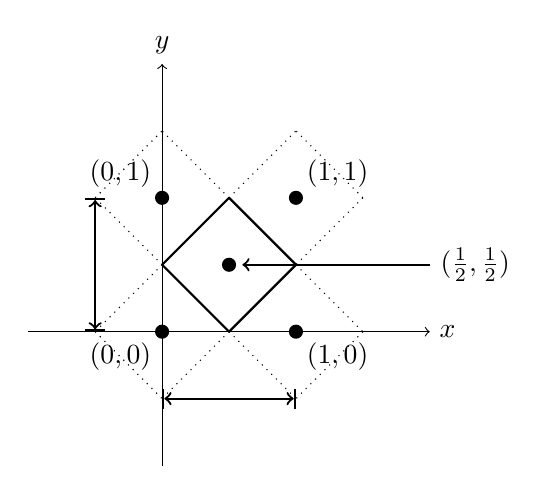
\begin{tikzpicture}[scale=1.7]
        \draw[->] (-1,0)--(2,0) node[right]{$x$};
        \draw[->] (0,-1)--(0,2) node[above]{$y$};
        
        \draw[thick] (0, 0.5) -- (0.5,0);
        \draw[thick]  (0.5,0) -- (1,0.5);
        \draw[thick]  (0,0.5) -- (0.5,1);
        \draw[thick]  (0.5,1) -- (1,0.5);
        
        \draw[thick,|<->|] (0,-0.5) -- (1,-0.5);
        \draw[thick,|<->|]  (-0.5,0) -- (-0.5,1);
        
         \fill (0.5,0.5)  circle[radius=1.5pt];
         \fill (0,0)  circle[radius=1.5pt] node[very thick, below left]{$(0,0)$};
         \fill (1,0)  circle[radius=1.5pt] node[very thick, below right]{$(1,0)$};
         \fill (0,1)  circle[radius=1.5pt] node[very thick, above left]{$(0,1)$};
         \fill (1,1)  circle[radius=1.5pt] node[very thick, above right]{$(1,1)$};
        
        \draw[thick,<-]  (0.6,0.5) -- (2,0.5) node[very thick, right]{$(\frac{1}{2},\frac{1}{2})$};
        
        \draw[dotted] (0.5,1) -- (0,1.5);
        \draw[dotted] (0,0.5) -- (-0.5,1);
        \draw[dotted] (-0.5,1) -- (0,1.5);
        
        \draw[dotted] (1.5,1) -- (1,1.5);
        \draw[dotted] (1.5,1) -- (1,0.5);
        \draw[dotted] (0.5,1) -- (1,1.5);
        
        \draw[dotted] (1,0.5) -- (1.5,0);
        \draw[dotted] (0.5,0) -- (1,-0.5);
        \draw[dotted] (1.5,0) -- (1,-0.5);
        
        \draw[dotted] (0,0.5) -- (-0.5,0);
        \draw[dotted] (0.5,0) -- (0,-0.5);
        \draw[dotted] (-0.5,0) -- (0,-0.5);

   \end{tikzpicture}
    \caption{$2$-dimension Voronoi cell centered at $(\frac{1}{2}, \frac{1}{2})$}
\end{figure}

\begin{plain}
\normalfont
The valid Voronoi cell (or Polyhedron generated by Diamond cutting algorithm) should have a volume (or area in $2$-dimensions) of $\frac{1}{2}$ \cite{481786}.
\end{plain}
Above implies that probability of $0, 1$ bits are both equal to $\frac{1}{2}$ in reconciled shared key. Since probability of vector to be inside or outside main Voronoi cell are equal, hence, there is no bias in generated key and it is uniformly distributed.

Below is a simple yet efficient procedure to check if vector generated by coefficients is in main Voronoi cell or otherwise. Subsequently, procedure finds the distance between coefficient vector and center of closest Voronoi cell. The procedure below is for $2$-dimensions, however, for $4$-dimensions it would be similar but $24$ inequalities to check instead of $4$ inequalities. To extract a key from a vector generated by coefficients, it would be similar but returning $1$ if vector is in main Voronoi cell and $0$ otherwise.



\begin{figure}[H]
\centering
% \begin{verbnobox}[\scriptsize]
%             if  (2.0, 2.0) · v - 1.0 >= 0    and (2.0, -2.0) · v + 1.0 >= 0  and
%                 (-1.0, -1.0) · v + 1.5 >= 0  and (-2.0, 2.0) · v + 1.0 >= 0)
        
%                 return (0.5, 0.5) - v
%             else
%                 return round(v) - v
% \end{verbnobox}


\begin{algorithm}[H]
    \caption{get\_distance\_voronoi\_cell}
    \begin{algorithmic}[1]
    \Procedure{get\_distance\_voronoi\_cell}{\textbf{v}}
        \State{\textbf{if} $(2.0, 2.0) \cdot \textbf{v} - 1.0 \ge 0$}
            \State \hspace{\algorithmicindent} $\text{ and } (2.0, -2.0) \cdot \textbf{v} + 1.0 \ge 0$
            \State \hspace{\algorithmicindent} $\text{ and } (-1.0, -1.0) \cdot \textbf{v} + 1.5 \ge 0$ 
            \State \hspace{\algorithmicindent} $\text{ and } (-2.0, 2.0) \cdot \textbf{v} + 1.0 \ge 0$
            \State \hspace{\algorithmicindent} \hspace{\algorithmicindent} \Return $(0.5, 0.5) - \textbf{v}$
        \State{\textbf{else}}
            \State \hspace{\algorithmicindent} \hspace{\algorithmicindent} \Return \texttt{round}(\textbf{v}) - \textbf{v}
    \EndProcedure
    \end{algorithmic}
    \end{algorithm}

    \caption{Finding distance between vector and center of closest Voronoi cell}
    \figuresubtitle{Note that above multiplications with vector \texttt{v} are dot product or scalar product. Also, \texttt{round} function, rounds $x, y$ components of vector \texttt{v} to nearest integer. As $x, y$ are in range $0 \le x, y < 1$ then result of \texttt{round} function would be $ \in \{ (0,0),(0,1),(1,0),(1,1) \}$}
\end{figure}

The idea that one party as a reconciliation information has to send array of (double precision) floating point numbers is not efficient. To resolve the issue Alkim at al. introduced the idea of splitting each Voronoi cells into \iftoggle{verylong}{$2^{rd}=$}{}$16$ sub-cells. Then instead of calculating the distance between vector generated by coefficients and center of closest Voronoi cell, we can find the closest center of Voronoi sub-cell (i.e. sub-cell number that coefficient is located at) and send the sub-cell number to other party as a reconciliation information. Then both parties will add the distance between  lattice point and center of sub-cell to the vector generated by their coefficients; hence they shift the vector generated by their coefficients toward center of their Voronoi cell. Therefore, instead of sending array of distances which are (double precision) floating point numbers, we can send the sub-cell numbers instead which are in integers. Note that we send the sub-cell number and not the outer Voronoi cell number to other party. As a result, eavesdropper does not learn anything from reconciliation information.







\begin{figure}[H]
    \centering
    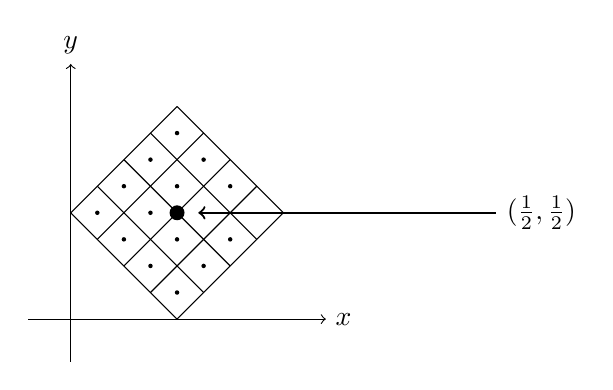
\begin{tikzpicture}[scale=2.7]
    
    \draw[->] (-0.2,0)--(1.2,0) node[right]{$x$};
    \draw[->] (0,-0.2)--(0,1.2) node[above]{$y$};
    
    
    \draw (0, 0.5) -- (0.5,0);
    \draw (0.5,0) -- (1,0.5);
    \draw (0,0.5) -- (0.5,1);
    \draw (0.5,1) -- (1,0.5);
    
    \draw (0.25,0.75) -- (0.75,0.25);
    \draw (0.375,0.875) -- (0.875,0.375);
    \draw (0.125,0.625) -- (0.625,0.125);
    
    \draw (0.125,0.375) -- (0.625,0.875);
    \draw (0.375,0.125) -- (0.875,0.625);
    \draw (0.250,0.250) -- (0.750,0.750);
    
    \fill (0.5,0.5)  circle[radius=1pt];
    \draw[thick,<-]  (0.6,0.5) -- (2,0.5) node[very thick, right]{$(\frac{1}{2},\frac{1}{2})$};
    

	\fill (0.5,0.875)  circle[radius=0.3pt];
	\fill (0.5,0.625)  circle[radius=0.3pt];
	\fill (0.625,0.5)  circle[radius=0.1pt];
	\fill (0.5,0.375)  circle[radius=0.3pt];
	\fill (0.5,0.125)  circle[radius=0.3pt];


	\fill (0.625,0.750)  circle[radius=0.3pt];
	\fill (0.750,0.625)  circle[radius=0.3pt];
	\fill (0.875,0.500)  circle[radius=0.1pt];

	\fill (0.750,0.375)  circle[radius=0.3pt];
	\fill (0.625,0.250)  circle[radius=0.3pt];
	\fill (0.375,0.250)  circle[radius=0.3pt];
	\fill (0.375,0.500)  circle[radius=0.3pt];
	\fill (0.375,0.750)  circle[radius=0.3pt];

	\fill (0.125,0.500)  circle[radius=0.3pt];
	\fill (0.250,0.625)  circle[radius=0.3pt];
	\fill (0.250,0.375)  circle[radius=0.3pt];

    \end{tikzpicture}
    \caption{$2$-dimension Voronoi cell centered at $ (\frac{1}{2}, \frac{1}{2} )$ split into 16 sub-cells}
\end{figure}

% \subsubsection{Concrete definition of reconciliation}

\iftoggle{long}{
For details on how NewHope reconciliation methods splits Voronoi cell into sub-cells and efficiently finds the sub-cells number in which vector generated by coefficients is located at, translating sub-cell number into Voronoi cell and subsequently extracting a bit form every $4$ coefficients refer to NewHope paper \cite{alkim2015post}.
}{}


\iftoggle{verylong}{
The following is the concrete description of $\mathrm{NewHope}$ reconciliation method. Let $\textbf{B} = (e_1, e_2, e_3, g)$ where $\textbf{g} = (\frac{1}{2}, \frac{1}{2}, \frac{1}{2}, \frac{1}{2})^{T}$ and $e_i$ is the $i$-th vector of unity. Moreover, let $D_4$ be the lattice defined by $\textbf{B}$. The $4$-dimensional space is divided into infinitely many four-dimensional cells, one cell for each lattice vector $\textbf{v}$. In the following we only look at four coordinates of the original vector $\textbf{v}_{R} \in \mathbb{Z}_{q}^{4}$, called $\textbf{v}^{(4)}_{R} \in \mathbb{Z}_{q}^{4}$. The coordinates of $\textbf{v}^{(4)}_{R}$ are divided by $q$ to obtain a vector $x \in \mathbb{R}^{4}/\mathbb{Z}^{4}$. In modulo $\mathbb{Z}^{4}$ there are only two cells in $\mathbb{R}^{4}$, the one corresponding to the lattice vector $\textbf{g}$ and the one corresponding to the lattice vector $(0, 0, 0, 0)^{T}$. If a vector $\textbf{x}$ lies in the cell which belongs to $\textbf{g}$, it is mapped to $1$, otherwise it is mapped to $0$. Determining the correct cell can be done by using algorithm $\mathrm{CVP}_{D_4}$. Since the sender and the receiver do not get exactly the same vectors $\textbf{v}_{S}^{(4)} \approx \textbf{v}_{R}^{(4)}$ that they want to encode in the way described above, they need to be sure that their vectors lie in the same cell. This however is not necessarily true. Hence, they need to exchange some reconciliation information $\textbf{c}^{(4)}$ which defines how the vector $\textbf{v}_{S}^{(4)}$ has to be moved to assure that it is in the same cell as $\textbf{v}_{R}^{(4)}$. For this we divide each cell into $2^{4r}$ sub-cells (if not stated differently, we assume $r = 2$). The receiver assigns the number of the sub-cell of $\textbf{v}_{R}^{(4)}$ to $\textbf{c}^{(4)} \in \{0, 1, 2, 3\}^{4}$ and sends it to the sender. Afterwards, the sender computes the difference vector of the middle of a cell and the middle of the sub-cell corresponding to $\textbf{c}$. Then the sender runs the $\mathrm{CVP}_{D_4}$ algorithm.

If $\textbf{v}_{S}^{(4)} \in \mathbb{Z}^{4}_{q}$ and $\textbf{c}^{(4)} \in \{0, 1, 2, 3\}^{4}$ then

\begin{equation}
\centering
    \mathrm{Rec}(\textbf{v}_{S}^{(4)}, \textbf{c}^{(4)}) = \mathrm{Decode}(\frac{1}{q} \textbf{v}_{S}^{(4)} - \frac{1}{2^r}\textbf{B}\textbf{c}^{(4)})
\end{equation}

computes one bit of the key from four coefficients.

% We identify an element $f(x) \in \mathbb{R}_{q}$ with a vector:
% \[(f_{0}', \dots, f_{\frac{n}{4}}') \in \mathbb{Z}[x] /(x^4 + 1)^{\frac{n}{4}} \text{ such that } f(x) = f'_{0}(x^{\frac{n}{4}}) + x \cdot f'_{1}(x^{\frac{n}{4}}) + \dots + x^{\frac{n}{4}} \cdot f'_{\frac{n}{4}}(x^{\frac{n}{4}})\]


The function $\mathrm{HelpRec}(\textbf{v}_{R})$ in the protocol of the receiver is defined as $\mathrm{HelpRec}(\textbf{v}_{R}^{(4)}) = \mathrm{CVP}_{D_4} (\frac{2^r}{q} (\textbf{v}_{R}^{(4)}) + b  \textbf{g}) \bmod 2^r$, where $b \leftarrow \{0, 1\}$.


\begin{algorithm}[H]
    \caption{CVP$_{D_{4}} (\textbf{x} \in \mathbb{R}^4)$}
    \begin{algorithmic}[1]
        \Procedure{CVP}{\textbf{x}}
            % \State \textbf{Ensure: } an integer vector $z$ such that $B \cdot z$ is closest to vector $x: x-B \cdot z \in \mathscr{V}$
            \State $\textbf{v}_{0} \leftarrow \lfloor \textbf{x} \rceil$
            \State $\textbf{v}_{1} \leftarrow \lfloor \textbf{x} - \textbf{g} \rceil$
            \State $k \leftarrow 0 \texttt{ if } ||\textbf{v} - \textbf{v}_{0}||_{1} < 1 \texttt{ else } 1$
            \State $(\textbf{v}_0, \textbf{v}_1, \textbf{v}_2, \textbf{v}_3)^{t} \leftarrow \textbf{v}_{k}$
            \State \textbf{return:} $(\textbf{v}_0, \textbf{v}_1, \textbf{v}_2, k)^{t} + \textbf{v}_{3} \cdot (-1, -1, -1, 2)^t$
        \EndProcedure
    \end{algorithmic}
\end{algorithm}

\begin{algorithm}[H]
    \caption{Decode $(x \in \mathbb{R}^4 / \mathbb{Z}^4)$}
    \begin{algorithmic}[1]
        \Procedure{Decode}{x}
            % \State \textbf{Ensure: } a bit $k$ such that $k \cdot g$ is closest vector to $x + \mathbb{Z}^4: x - kg \in \mathscr{V} + \mathbb{Z}^4$
            \State $\textbf{v} \leftarrow \textbf{x} - \lfloor \textbf{x} \rceil$
            \State $r \leftarrow  0 \texttt{ if } ||\textbf{v}||_{1} \le 1 \texttt{ else } 1$
            \State \textbf{return:} $r$
        \EndProcedure
    \end{algorithmic}
\end{algorithm}
}

Furthermore, NewHope protocol generates the shared polynomial pseudo-randomly on every run of the KEM to assure safety against backdoors. Next chapter discusses the method as suggest in NewHope protocol to efficiently share the shared polynomial with other party. In essence, to generate a pseudo-random polynomial $A$, NewHope uses a $256$-bit seed and a type of hash-function that outputs arbitrary length, e.g., $\mathrm{SHAKE}$-128. This can be done similarly for all the other protocols.





\subsubsection{Generalized form of randomized doubling function suggested by Alkim et al.}
The probability of $\textbf{x}$ being in a center Voronoi cell is the same as for $\textbf{x}$ being in other Voronoi cells. This would be the case if $\textbf{x}$ actually followed a continuous uniform distribution. However, the coefficients of $\textbf{x}$ are discrete values in $\{0,\frac{1}{q},\dots,\frac{q-1}{q}\}$ and with the protocol described so far, the bits of $\textbf{v}$ would have a small bias. The solution is to add to $\textbf{x}$ with probability $\frac{1}{2}$ the vector $(\frac{1}{2q}, \dots, \frac{1}{2q})$ before running the error reconciliation. This has close to no effect for most values of $\textbf{x}$, but, with probability $\frac{1}{2}$ moves $\textbf{x}$ to another Voronoi cell if it is very close to one side of a border.

In the example below we see that $72$ dots ($36$ red and $36$ black ones) remain in their Voronoi cell; the other $9$ dots ($4$ red and $5$ black ones) change Voronoi cell with probability $\frac{1}{2}$ which precisely eliminates the bias in the key.

\begin{figure}[H]
\centering
\includegraphics[scale=0.3]{dbl_newhope}
\caption{Effect of generalized form of randomized doubling function on vectors}
\end{figure}








    \section{\texorpdfstring{$\mathrm{BCNS}$}{BCNS} and \texorpdfstring{$\mathrm{NewHope}$}{NewHope} diagram comparison}
The basic sketch of both $\mathrm{BCNS}$ and $\mathrm{NewHope}$ protocols are very similar to Ding's key-exchange protocol ($\mathrm{DXL}$). They all share the basics, initiator sends a polynomial $b$ to responder and responder replies by sending $b', c$ where $c$ is a reconciliation information or a bit string to improve success probability of key-agreement. For every coefficient of responder's calculated key, there is one reconciliation bit and there are at most $1024$ coefficients. Therefore, responder is sending at most $1024$ bits as a reconciliation information.

\begin{figure}[H]
    \centering
	\begin{tabular}{|lll|}
		\hline
		$a \leftarrow \text{Uniformly random}$          &                      &                                                                    \\\hline
		\textbf{Alice}                                  &                      & \textbf{Bob}                                                       \\\hline
		$s, e \xleftarrow{\$} \chi$                     &                      & $s', e' \xleftarrow{\$} \chi$                                      \\
		$b \leftarrow as + e$                           & $\xrightarrow{b}$    & $b' \leftarrow as' + e'$                                           \\
		                                                &                      & $e'' \xleftarrow{\$}\chi$                                          \\
		                                                &                      & $v \leftarrow bs' + e''$                                           \\
		                                                & $\xleftarrow{b', c}$ & $\bar{v} \xleftarrow{\$}\text{dbl(v)}$                            \\
		                                                &                      & $c \leftarrow \langle \bar{v} \rangle_{2q, 2} \in \{0, 1\}^{n}$    \\
% 		$k_{A} \leftarrow rec(2b's, c)\in \{0, 1\}^{n}$ &                      & $k_{B} \leftarrow \lfloor \bar{v} \rfloor_{2q, 2}\in \{0, 1\}^{n}$ \\\hline
	    $k_{A} \leftarrow \text{rec}(2b's, c)\in \{0, 1\}^{n}$ &                      & $k_B \leftarrow \text{rec}(2bs', c) \in \{0, 1\}^n$                       \\\hline
	\end{tabular}
	\caption{Diagram of $\mathrm{BCNS}$ protocol}
\end{figure}



In $\mathrm{NewHope}$ protocol however, initiator also sends a \textit{seed} derived from a uniformly random distribution that enables the other party to deterministically create a shared polynomial by themselves without actually sending it. This is results in an efficiency in bandwidth needed for key-exchange. Also, to make sure the resulting shared key is uniformly random or number of $0$'s and $1$'s are uniformly distributed, NewHope uses $\mathrm{SHA}$-3. Note that if number of $0$'s and $1$'s are always exactly equal then we can deterministically find the shared key. Using a hash function will not have any impact on hardness of Ring-$\mathrm{LWE}$, it is just matter of making bits of resulting shared key uniformly distributed and making a sure it is irreversible (i.e. eavesdropper needs to break $\mathrm{SHA}$-3 first and then would be able to break Ring-$\mathrm{LWE}$). 

Another important observation is reconciliation information of $\mathrm{NewHope}$ is slightly different from $\mathrm{BCNS}$ protocol. In NewHope, one party sends a sub-cell number calculated from coordinate tuple generated by every $4$ coefficients to other party. Further, $\mathrm{NewHope}$ protocol divides each Voronoi cell to $16$ sub-cells so for every $4$ coefficient it requires up-to $4$ bits. Considering that there are total of up-to $1024$ coefficients in responder's key then responder is in fact sending $256 \times 4 = 1024$ bits as a reconciliation information, which is the same number of bits as in $\mathrm{BCNS}$ protocol.

\begin{figure}[H]
	\centering
	\begin{tabular}{|lll|}
		\hline
		$q = 12289 < 2^{14}, n = 1024, \Psi_{16}$           &                          &                                                     \\\hline
		\textbf{Alice}                                      &                          & \textbf{Bob}                                        \\\hline
		$seed \xleftarrow{\$} \{0, 1\}^{256}$               &                          &                                                     \\
		$a \leftarrow \text{parse}(\text{SHAKE-128}(seed))$ &                          &                                                     \\
		$s, e \xleftarrow{\$} \Psi_{16}^{n}$                &                          & $s', e', e'' \xleftarrow{\$} \Psi_{16}^{n}$          \\
		$b \leftarrow as + e$                               & $\xrightarrow{(b, seed)}$& $a \leftarrow \text{parse}(\text{SHAKE-128}(seed))$ \\
		                                                    &                          & $u \leftarrow as' + e'$                             \\
		                                                    &                          & $v \leftarrow bs' + e''$                            \\
		$v' \leftarrow us$                                  & $\xleftarrow{(u, r)}$    & $r \xleftarrow{\$}\text{HelpRec}(v)$                \\
		$v \leftarrow \text{Rec}(v', r)$                    &                          & $v \leftarrow \text{Rec}(v, r)$                     \\
		$\mu \leftarrow \text{SHA3-256}(v)$                 &                          & $\mu \leftarrow \text{SHA3-256}(v)$                 \\\hline
	\end{tabular}
	\caption{Diagram of $\mathrm{NewHope}$ protocol}
\end{figure}


With regards to $e''$ added to Bob's calculated key and the reason for it, notice if $e''$ is not there, then $v=bs'$ in both protocols, which means it would be easy to recover $s'$ given $v$ and $b$. Since $b$ is sent in the clear over the channel, and a (randomized) function of $v$ appears in the clear as $c$ (or $r$), without using $e''$ to hide $s'$, information about $s'$ would likely be leaked both to Alice and to any eavesdropper of the channel. Even if it would not immediately leak all of $s'$, any leakage is clearly bad. As a result, $e''$ is used to make sure that $v = bs' + e''$ is indistinguishable from random, i.e. the distribution of $v$ is independent of $s'$, assuming Ring-$\mathrm{LWE}$ is hard. See also the security proof in the $\mathrm{BCNS}$ paper \cite{bos2015post}, where Game 1 and Game 2 are assumed to be indistinguishable under the Ring-$\mathrm{LWE}$ assumption. The reason Alice does not add some $e''$ as well is because Alice uses $e$ to hide her own secret $s$, just like Bob uses $e'$ to hide his secret $s'$. To agree on the key (both parties have different noise on the shared key, which they do not wish to disclose). Bob has to send this extra key reconciliation message, for which he again hides his secret $s'$ with fresh random noise $e''$.


    \section{Parameter choices for Ring-\texorpdfstring{$\mathrm{LWE}$}{LWE} key-exchange}
The Ring-$\mathrm{LWE}$ key-exchange presented above worked in the Ring of polynomials of degree $n-1$ or less $\bmod$ a polynomial $\Phi(x)$. Note that $n$ is a power of $2$ and $q$ is a prime which is congruent to $1 \bmod 2n$. Following the guidance given in Peikert's paper \cite{peikert2014lattice}, V. Singh in \cite{vikramsingh2015} suggested two sets of parameters for the RLWE-KEX and in both coefficient of error polynomial is sampled from normal distribution with standard deviation $\sigma = \frac{8}{\sqrt{2\pi}}$. Suggested parameters are as follows:

\begin{enumerate}
    \item For $128$ bits of security, $n = 512$, $q = 25601$, and $\Phi(x) = x^{512} + 1$
    \item For $256$ bits of security, $n = 1024$, $q = 40961$, and $\Phi(x) = x^{1024} + 1$
\end{enumerate}

Because RLWE based key exchange uses random sampling and fixed bounds, there is a small probability that the key-exchange will fail to produce the same key for the initiator and responder. Given Gaussian parameter $\sigma$ equals to $\frac{8}{\sqrt{2 \pi}} = 3.192$, Singh in \cite{vikramsingh2015} calculated that probability of key agreement failure to be less than $2^{-71}$ for the $128$-bit secure parameters and less than $2^{-91}$ for the $256$-bit secure parameters. $\mathrm{BCNS}$ protocol kept the $\sigma$ and $\Phi$ as suggested by Singh for $256$ bits of security, but changed the prime modulus of finite field to $2^{32}-1$. This resulted in failure probability of $2^{-131072}$. 

Originally (in early versions of protocol), $\mathrm{NewHope}$ kept the $\Phi$ as suggested by Singh, but used $12$-bit binomial distribution instead with $\sigma = \sqrt{\frac{12}{2}} = 2.449$ and changed the prime modulus of finite field to $12289$. This represents a $70\%$ reduction in public key size over the parameters of Singh. Hence, reducing the prime modulus size resulted in failure probability of $2^{-105}$. But in later version (and after discussion with A. Langley from Google), Alkim et al. used $16$-bit binomial distribution with $\sigma = \sqrt{\frac{16}{2}} = 2.828$ which resulted in failure probability of $2^{-60}$. In fact, this later parameter was implemented in Google's Chrome Canary project as well as Boring-SSL which is a fork of Open-SSL that is designed to meet Google's needs \cite{braithwaite_2016}.

\begin{plain}
\normalfont
Notice the smaller $q$ results in faster key-exchange by reducing over-head size and increase in security, and most importantly increasing impact of error terms, but this yields higher failure probability.
\end{plain}



\begin{table}[H]
	\centering
	\begin{adjustbox}{width=1\textwidth}
		\small
		\begin{tabular}{|l|l|l|l|l|l|l|l|l|l|}
			\hline
			$n$  & $q$        & Distribution & Parameter            & Security Claim & Rec. Algorithm     & Citation                      \\ \hline
			512  & 1051649    & Gaussian     & $3.19 / \sqrt{2\pi}$ & $2^{128}$      & $\mathrm{DXL}$     & \cite{cryptoeprint:2015:008}  \\ \hline
			820  & 49261      & Gaussian     & $8 / \sqrt{2\pi}$    & $2^{256}$      & $\mathrm{Peikert}$ & \cite{cryptoeprint:2015:1120} \\ \hline
			1024 & 12289      & Binomial     & $\sqrt{{16} / {2}}$  & $\> 2^{128}$   & $\mathrm{NewHope}$ & \cite{alkim2015post}          \\ \hline
			1024 & 40961      & Gaussian     & $8 / \sqrt{2\pi}$    & $\> 2^{256}$   & $\mathrm{Peikert}$ & \cite{cryptoeprint:2015:1120} \\ \hline
			1024 & $2^{32}-1$ & Gaussian     & $8 / \sqrt{2\pi}$    & $\> 2^{128}$   & $\mathrm{Peikert}$ & \cite{bos2015post}            \\ \hline
		\end{tabular}
	\end{adjustbox}
	\caption{Listing of a number of different parameter choices for KEXs using the Ring Learning with Errors problem}
\end{table} 

    \section{Lattice based authenticated key-exchange}
Key-exchange protocol (KEX) is a cryptographic primitive to derive a common secret key via a public network communication between a number of parties. The parties do not share any secret information beforehand. KEX that also authenticates the identities of the involved parties is called authenticated key-exchange protocol (AKE). More formally, in an AKE protocol each party has a static public-secret key pair. The static public key is certified with the party's identity. When running the protocol, each party generates an ephemeral secret key and, depending on that, a corresponding ephemeral public key. The public key is sent to the other party. Each party computes a shared session key by using the ephemeral key and the static key (e.g. password).

An authenticated key-exchange protocol is said to have perfect forward secrecy (PFS) if a compromise of its static keys does not lead to a compromise of previously established and deleted session keys. There are many existing authenticated key-exchange approaches built for Diffie-Hellman, however they all can be used with Ring-$\mathrm{LWE}$ instead because of similarities in design. Authenticated key-exchange aims to overcome man-in-the-middle attack, which is an attack where the attacker secretly relays and possibly alters the communication between two parties who believe they are directly communicating with each other. The following are basic authenticated Diffie-Hellman approaches that can be applied to RLWE-KEX:

\begin{enumerate}
    \item Use key-exchange in conjunction with a signing certificate (use either RSA or DSA as a public key). The server sends its certificate which client validates and ephemeral key signed (or encrypted) using server's private key. Client validates the ephemeral key using certificate and encrypts the session using ephemeral key. 
    \item Concatenate (or pad) ephemeral key (or result of unauthenticated key-exchange) with a password and use the hash of that as a session key to achieve a secure communication
    \item Encrypt $b = A s + e$ (in Ring-$\mathrm{LWE}$) or $K = g^a \bmod p$ (in Diffie-Hellman) using a password as an encryption key before sending it to other party.
\end{enumerate}
    
\chapter{Implementation specifications}
    In this chapter, we overview specifics of Ring-$\mathrm{LWE}$ based protocols which includes: methods of error sampling, methods to generate shared polynomial between two parties and performance analysis. The goal of this chapter is to explain in details how key-exchange reconciliations that was discussed in previous chapter was implemented as a protocol.


\section{Error sampling algorithm}
Lattice based cryptography began with the seminal work of Ajtai, who built a one-way function based on the worst-case hardness based on certain lattice problems \cite{ajtai1996generating}. These lattice problems are believed to be hard even in the presence of large quantum computers and such a promising post-quantum replacement for standard cryptography. The most general public key primitives like encryption schemes \cite{cryptoeprint:2012:230} and digital signatures \cite{cryptoeprint:2011:537} already have practical lattice based instantiations.

Many recent lattice based schemes require sampling from discrete Gaussian. The parameters of discrete Gaussian are governed by the security proofs of the particular schemes. A finite machine cannot sample from a discrete Gaussian distribution, hence one has to sample from a distribution close to it. It is a common practice to require that the statistical distance of the sampled distribution from the desired discrete Gaussian be less than $2^{-100}$.

Computing the probabilities requires floating point operations of at least $100$ bit precision if one wants to achieve a statistical distance less than $2^{-100}$ \cite{Janos2014}. Whereas any precomputation means storing a variable amount of values of the same precision. This can highly affect the sampling performance on personal computers and even make the implementation completely impractical on constrained devices. Weiden et al. \cite{cryptoeprint:2013:065} report that the Gaussian sampling takes up 50\% of the running time of Lyubashevsky's signature scheme (also known as BLISS) \cite{cryptoeprint:2011:537}. Thus efficient sampling from discrete Gaussians plays a crucial role in the performance
of these primitives.

S. Galbraith in \cite{Dwarakanath:2014:SDG:2635676.2635683} discussed different discrete Gaussian sampling algorithms suitable for constrained devices. By a constrained device we can think of an embedded or portable device with a small amount of memory (measured in kilobytes instead of gigabytes) and a modest processor that has to be economical with respect to power usage. Also these kind of devices do not necessarily come with floating point arithmetic capability. Even if a platform provides floating point arithmetic, the required precision is usually not supported natively. This means that software libraries have to be used for this functionality, and these can significantly worsen performance and take up additional space in the already tight memory.

A particular discrete Gaussian samplers may apply different techniques to increase the performance and reduce or even avoid the floating point operations, which usually utilize precomputed tables, hence not requiring floating point arithmetic. Many factors can affect the performance and memory consumption (i.e., the size and number of the potential precomputed tables). Such factors are the size of the Gaussian parameter, whether the center is zero or not, and whether the parameters are fixed or changing (or more precisely, the number of the needed parameter combinations). To evaluate the practicality of the discrete Gaussian samplers in lattice based cryptography one needs to assess the parameters of the distributions required by the different cryptographic
schemes.

The techniques utilized by different samplers require various amount of memory and floating point operations, which results in different overall performance on the particular platforms. Thus for the evaluation of their practical performance one needs to collect the characteristics of the discrete Gaussian samplers too.

% \begin{definition}
% \normalfont
% Discrete probability function (or PDF), $p(x)$, is a function that satisfies the following properties.

% \begin{enumerate}
%     \item Let $X$ be a discrete random variables. The probability that $x$ can take a specific value is $p(x)$. That is: $P[X=x]=p(x)$
%     \item $p(x)$ is non-negative for all real $x$
%     \item The sum of $p(x)$ over all possible values of $x$ is $1$, that is $\sum_{j} p_{j} = 1$ where $j$ represents all possible values that $x$ can have and $p_j$ is the probability at $x_j$
% \end{enumerate}
% \end{definition}

% One consequence of properties ($2$) and ($3$) is that $0 \le p(x) \le 1$. What it actually means is that discrete probability function is a function that can take a discrete number of values (not necessarily finite). This is most often the non-negative integers or some subset of the non-negative integers. There is no mathematical restriction that discrete probability functions only be defined at integers, but in practice this is usually what makes sense. Each of the discrete values has a certain probability of occurrence that is between zero and one. That is, a discrete function that allows negative values or values greater than one is not a probability function. The condition that the probabilities sum to one means that at least one of the values has to occur.

% \begin{definition}
% \normalfont
% The cumulative distribution function ($\mathrm{CDF}$) is the probability that the variable takes a value less than or equal to $x$. That is: $Pr[X \le x]= \alpha$. For a discrete distribution, the $\mathrm{CDF}$ can be expressed as: $\sum_{i = 0}^{x}f(i)$
% \end{definition}

In the following by PDF and CDF we are referring to \textit{Probability Density Function} and \textit{Cumulative Distribution Function}. Note that the relation between the probability density function $f$ and the cumulative distribution function $F$ is $F(k) = \sum_{i \le k} f(i)$ if $f$ is discrete and  $F(x) = \int_{y \le x} f(y)\,dy$ if $f$ is continuous.



\begin{definition}
\normalfont
The probability density of the normal distribution is:
$f(x\;|\;\mu ,\sigma ^{2})={\frac {1}{\sqrt {2\sigma ^{2}\pi }}}\;e^{-{\frac {(x-\mu )^{2}}{2\sigma ^{2}}}}$

Where:
\begin{itemize}
    \item $\mu$ is mean or expectation of the distribution (center of $\mathrm{PDF}$)
    \item $\sigma$ is standard deviation
    \item $\sigma^{2}$ is variance
\end{itemize}
\end{definition}

\begin{plain}
\normalfont
Coefficients of polynomials in Ring-$\mathrm{LWE}$ are $\in \mathbb{Z}$. Therefore, error sampling methods should sample from \textit{Discrete Distributions} as oppose to \textit{Continuous Distributions}.
\end{plain}

\subsection{Inversion sampling}
Inverse transform sampling (also known as Smirnov transform) is a basic method for pseudo-random number sampling, i.e. for generating sample numbers at random from any probability distribution given its cumulative distribution function.

Inverse transformation sampling takes uniform samples of a number $u$ between $0$ and $1$, interpreted as a probability, and then returns the largest number $x$ from the domain of the distribution $P(X)$ such that $P(-\infty <X<x)\leq u$.

In this method, we are randomly choosing a proportion of the area under the curve and returning the number in the domain such that exactly this proportion of the area occurs to the left of that number. Intuitively, we are unlikely to choose a number in the far end of tails because there is very little area in them which would require choosing a number very close to zero or one.

Computationally, this method involves computing the quantile function of the distribution; in other words, computing the cumulative distribution function ($\mathrm{CDF}$) of the distribution (which maps a number in the domain to a probability between $0$ and $1$) and then inverting that function. This is the source of the term \quotes{inverse} or \quotes{inversion} in most of the names for this method. Note that for a discrete distribution, computing the CDF is not in general too difficult: we simply add up the individual probabilities for the various points of the distribution. For a continuous distribution, however, we need to integrate the probability density function ($\mathrm{PDF}$) of the distribution, which is impossible to do analytically for most distributions including the normal distribution. As a result, this method may be computationally inefficient for many distributions and other methods are preferred.

For the normal distribution, the lack of an analytical expression for the corresponding quantile function means that other methods may be preferred computationally. It is often the case that, even for simple distributions, the inverse transform sampling method can be improved on, for example, the ziggurat algorithm and rejection sampling \cite{Janos2014}.

\subsubsection{Naive sampling approach using \texorpdfstring{$\mathrm{PDF}$}{PDF} function}
One simple approach which generates only positive integer samples is calculating probabilities using $\mathrm{PDF}(x)$ $\forall x \in [0, \text{variance}]$ and putting them in an array. Note that, sum of probability array would not be equal to one because we ignored the probabilities of negative values. Thereafter, we need to normalize the probability array such that sum would equal to $1$. Then, create a new array with the same size as probability array but setting first element of new array as first element of probability array. Thereafter, we set new array at any index to sum of probability array until that index. We can call the probability array, vector of $\mathrm{PDF}$ values and also call second array, vector of $\mathrm{CDF}$ values. Note that value of last element of $\mathrm{CDF}$ vector should equal to $1$ because we normalized the probability list and sum of probability list should equal to $1$. 

To sample integers in range $[0, \text{variance}]$ using this method, simply generate a random number between $[0, 1)$ uniformly at random, lets call it $u$. Then find a index such that $u < \mathrm{CDF}[index]$. The value of \textit{index} is a sample from the distribution.

Below is an implementation of the naive Gaussian sampler that we described above; centered at $0$ with $\sigma = \frac{8}{\sqrt{2  \pi}}$ as suggested in early draft of $\mathrm{BCNS}$ protocol.



\begin{algorithm}[H]
    \caption{naive Gaussian sampler by estimating cdf values}
    \begin{algorithmic}[1]
        \State sigma $\gets 8 / \sqrt{2  \pi}$ 
        \State variance $\gets \text{sigma}^2$
        \State mu $\gets 0$
        \State domain $\gets$ $\lceil\text{variance}\rceil$
        \item[] \Comment{probability density of the normal distribution}
        \Function{pdf}{x}
            \State \textbf{return:} $(1/\sqrt{2 \pi \times \text{variance}}) \times e^{-{(x - \text{mu})}^2 / (2 \times \text{variance})}$
        \EndFunction
        \item[] \Comment{note that sum of probabilities that this function generates is equal to 1/2}
        \item[] \Comment{because we are ignoring probabilities of negative numbers}
        \Function{create\_pdf\_vector}{}
            \State pdf\_vector $\gets$ empty array of size $=$ domain
            \For{ $x \gets 0 \text{ to domain}$ }
                \State pdf\_vector[x] $\gets$ pdf(x)
            \EndFor
            \State \textbf{return:} pdf\_vector
        \EndFunction
        \item[] \Comment{normalize probability list such that sum of probability would equal to 1}
        \Function{normalize\_pdf\_vector}{pdf\_vector}
            \State $s \gets$ sum(pdf\_vector)
            \For{ $i \gets 0 \text{ to domain}$ }
                \State pdf\_vector[$i$] = pdf\_vector[$i$] $/ \text{sum}$ 
                \State $i \gets i + 1$
            \EndFor
            \State \textbf{return:} pdf\_vector
        \EndFunction
        \item[] \Comment{create cdf vector from pdf\_vector}
        \Function{create\_cdf\_vector}{pdf\_vector}
            \State cdf\_vector $\gets$ empty array of size $=$ domain
            \State total $\gets 0$
            \For{ $i \gets 0 \text{ to } \text{domain}$ }
                \State total $\gets$ total + pdf\_vector[$i$]
                \State cdf\_vector[$i$] $\gets$ total
            \EndFor
            \State \textbf{return:} cdf\_vector
        \EndFunction
        \algstore{example1}
    \end{algorithmic}
\end{algorithm}

\begin{algorithm}[H]
    \begin{algorithmic}
        \algrestore{example1}
        \item[] \Comment{sample from cdf\_vector}
        \Function{sample}{}
            \State rand $\gets$ select a number in range $[0, 1)$ uniformly random
            \State index $\gets 0$
            \While{ $\text{rand} > \text{cdf\_vector[index]}$ }
                \State index $\gets$ index $+ 1$
            \EndWhile
            \State \textbf{return:} index
        \EndFunction
        \item[] \Comment{initialize the sampler}
        \State pdf\_vector $\gets$ create\_pdf\_vector()
        \State pdf\_vector $\gets$ normalize\_pdf\_vector(pdf\_vector)
        \State cdf\_vector $\gets$ create\_cdf\_vector(pdf\_vector)
        \State s $\gets$ sample(cdf\_vector)
    \end{algorithmic}
\end{algorithm}

\iftoggle{verylong}{
\lstinputlisting[language=Python, caption=Naive Gaussian sampler]{code_snippets/naive_gaussian_sampler.sage}
}{}

\begin{figure}[H]
\centering
\includegraphics[scale=0.3]{naive-samples}
\caption{Plot (or histogram) of Gaussian samples using the naive method}
\figuresubtitle{Above is centered at $0$ and $\sigma = \frac{8}{\sqrt{2  \pi}}$}
\end{figure}



\subsubsection{Inversion sampling using \texorpdfstring{$\mathrm{PDF}$}{PDF} function and bisection search}
Above method can be improved using Taylor approximation to estimate the $\mathrm{CDF}$ and bisection search to estimate the inverse of $\mathrm{CDF}$. It is important to note that $\mathrm{CDF}$ function of normal distribution is not invertible so to calculate the inverse of $\mathrm{CDF}$ function we need to use Taylor series to find the integral (or area under the graph) of $\mathrm{PDF}$ function.

The bisection search method is a root-finding method that repeatedly bisects an interval and then selects a sub-interval in which a root must lie for further processing. It is a very simple and robust method, but it is also relatively slow. Because of this, it is often used to obtain a rough approximation to a solution which is then used as a starting point for more rapidly converging methods. This method is also called the interval halving method. Bisection search method does not really takes the advantage of the fact that coefficients of error polynomial are integers, so we need to round the sample to nearest integer which is not the most efficient approach. Also, to calculate the inverse of $\mathrm{CDF}$ we are constantly calculating $\mathrm{CDF}$ and also so we are not storing the $\mathrm{CDF}$ values (memorizing concept) of particular probability. As a result, this approach is very slow.


\begin{algorithm}[H]
    \caption{Gaussian sampler using Taylor series and bisection search}
    \begin{algorithmic}[1]
        \State sigma $\leftarrow 8 / \sqrt{2  \pi}$, variance $\leftarrow \text{sigma}^2$
        \item[] \Comment{probability density of the normal distribution}
        \Function{pdf}{x}
            \Return $(1/\sqrt{2 \pi \times \text{variance}}) \times e^{-{(x - \text{mu})}^2 / (2 \times \text{variance})}$
        \EndFunction
        \item[] \Comment{calculates cumulative distribution using Taylor approximation}
        \Function{cdf}{x}
            \If{x $<$ -1 $\times$ variance}
                \Return 0.0
            \ElsIf{x $>$ variance}
                \Return 1.0
            \EndIf
            \State sum $\leftarrow$ 0.0
            \State term $\leftarrow x$
            \State $i \leftarrow 3$
            \While{sum + term $\neq$ sum}
                \State sum $\leftarrow$ sum + term
                \State term $\leftarrow$ term $\times x^2 / i$
                \State $i \leftarrow i + 2$
            \EndWhile
            \Return $0.5 + $ sum $\times$ pdf(x)
        \EndFunction
        \item[] \Comment{bisection search to find a value $y$ such that it's CDF equals to $x$}
        \Function{inverse\_cdf}{x, delta, lo, hi}
            \State mid $\leftarrow$ lo $+$ (hi $-$ lo) $/ 2$
            \If{hi $-$ lo $<$ delta} \Return mid
            \ElsIf{cdf(mid) $>$ x}
                \State \Return inverse\_cdf(x, delta, lo, mid)
            \Else \text{ }
                \State \Return inverse\_cdf(x, delta, mid, hi)
            \EndIf
        \EndFunction
        \item[] \Comment{initialize the bisection search}
        \Function{inverse\_cdf\_init}{x}
            \State mid $\leftarrow$ lo $+$ (hi $-$ lo) $/ 2$
            \State \Return inverse\_cdf(x, 0.00000001, -variance, variance)
        \EndFunction
        \algstore{example2}
    \end{algorithmic}
\end{algorithm}



\begin{algorithm}[H]
    \begin{algorithmic}
        \algrestore{example2}
        \item[] \Comment{sample from Gaussian by generating a random number and find it's inverse of CDF}
        \Function{sample}{}
            \State $x \leftarrow $ generate a number between $[0, 1)$ uniformly random
            \State \Return inverse\_cdf(x, variance)
        \EndFunction
        \item[] \Comment{initialize the sampler}
        \State pdf\_vector $\leftarrow$ create\_pdf\_vector()
        \State pdf\_vector $\leftarrow$ normalize\_pdf\_vector(pdf\_vector)
        \State cdf\_vector $\leftarrow$ create\_cdf\_vector(pdf\_vector)
        \State s $\leftarrow$ sample(cdf\_vector)
    \end{algorithmic}
\end{algorithm}

\iftoggle{verylong}{
\lstinputlisting[language=Python, caption=Improved Gaussian sampler]{code_snippets/inversion_sampling_gaussian.sage}
}{}

\begin{figure}[H]
\centering
\includegraphics[scale=0.3]{improved_sampler}
\caption{Plot (or histogram) Gaussian sampler using bisection search and Taylor series}
\figuresubtitle{Above is centered at $\text{variance}^2$, $\sigma = \frac{8}{\sqrt{2  \pi}}$}
\end{figure}

\subsubsection{Inversion sampling using pre-calculated \texorpdfstring{$\mathrm{CDF}$}{CDF} table}
$\mathrm{BCNS}$ protocol uses inversion sampling with pre-computed look-up table of $\mathrm{CDF}$. If look-up table was not available, then we had to calculate the $\mathrm{CDF}$. The specification of $\mathrm{CDF}$ look-up table is the following:

\begin{equation}
    \begin{aligned}
        \text{table}[0] = 2^{189}  \\
        \text{table}[51] = 2^{192}\\
        \text{table}[i] < \text{table}[i+1] : \forall_{i} \in 0 \le i \le 50
    \end{aligned}
\end{equation}


To samples form this look-up table, we independently generate a $192$-bit integer $v_{j}$ uniformly at random, and compute the unique smallest integer index $ind_{j} \in [0, 50]$ such that $v_{j} < \text{table}[ind_{j}]$. We then generate one additional random bit to decide the sign $sign_{j} \in \{-1, 1\}$, and return the $j$-th coefficient as $s_{j} \leftarrow sign_{j} \times ind_{j}$. $\mathrm{BCNS}$ uses little Endian memory storing format (i.e. 192 bits stored as \texttt{struct} of $3 \times 64 = 192 $ bits) to store the array. Little endians in essence means storing the least significant byte in the smallest address.


\begin{algorithm}[H]
    \caption{gaussian sampler given CDF table as written in $\mathrm{BCNS}$ protocol}
    \begin{algorithmic}[1]
        \State rlwe\_table $\leftarrow$ $52 \times 3$ matrix of 64 bit little endians
        \State big\_integers $\leftarrow$ empty array with size equals to number of rows in rlwe\_table (i.e. 52)
        \item[] \Comment{convert little-endian as stored above to Big-endian}
        \Function{little\_to\_big\_endian}{}
            \For{$ i \gets 0 \text{ to } \text{height of rlwe\_table}$}
                \State big $\leftarrow 0$
                \For{$ j \gets 0 \text{ to } \text{width of rlwe\_table}$}
                    \State big $\leftarrow$ big \texttt{OR} (rlwe\_table[$i$][$j$] \texttt{LSHIFT} ($j \times 64$))
                \EndFor
                \State big\_integers[$i$] $\leftarrow$ big
            \EndFor
            \State \Return big\_integers
        \EndFunction
        \item[]
        \item[] \Comment{this function uses bits that are sampled uniformly at random to sample Gaussian}
        \Function{sample}{}
            \State $n \leftarrow $ get a 192 bits uniformly random
            \State $i \leftarrow 0$
            \For{$i \gets 0 \text{ to } \text{length(big\_integers)}$}
                \If{$n < $ big\_integers[$i$]}
                    \State \Return $i$
                \EndIf
            \EndFor
        \EndFunction
    \end{algorithmic}
\end{algorithm}

\iftoggle{verylong}{
\lstinputlisting[language=Python, caption=Gaussian sampler using pre-calculated table of CDF]{code_snippets/inversion_sampling_given_cdf.sage}
}{}

\begin{figure}[H]
\centering
\includegraphics[scale=0.3]{cdf-table-BCNS.png}
\caption{Plot of precomputed $\mathrm{CDF}$ table as implemented in $\mathrm{BCNS}$ protocol}
\figuresubtitle{Notice the last column is just $1$s.}
\end{figure}


\begin{figure}[H]
\centering
\includegraphics[scale=0.3]{samples-from-BCNS.png}
\caption{Plot (or histogram) of $\mathrm{BCNS}$ Gaussian sampler}
\figuresubtitle{Close to a perfect discrete Gaussian sampler (statistical difference $<2^{-128}$)}
\end{figure}




\subsection{Binomial distribution}
$\mathrm{NewHope}$ protocol uses binomial distribution ($\Psi_{16}$) as oppose to Gaussian distribution for efficiency reasons. Interestingly, difference of two independently uniformly sampled random variables is a binomial distribution sample when bits are uniformly sampled. The method they use is to sample $b$, $b'$ each $16$ bits, then their difference forms a binomial distribution sample centered at zero. This distribution has standard deviation $\sigma = \sqrt{\frac{k}{2}}$, where $k$ is number of bits. In the paper \cite{alkim2015post}, Alkim et al. provides a proof that such a binomial distribution is a good approximation of Gaussian distribution.  


\begin{figure}[H]
\centering
\includegraphics[scale=0.3]{binomial-distribution-shifted.png}
\caption{Plot of Binomial distribution $\Psi_{8}$, shifted for visualization purposes}
\figuresubtitle{This binomial distribution would have a standard deviation of $\sigma = \sqrt{\frac{8}{2}}$}
\end{figure}


\begin{algorithm}[H]
    \begin{algorithmic}[1]
        \caption{Binomial distribution sampler with $\Psi_{16}$ as written in $\mathrm{NewHope}$ protocol}
        \item[] \Comment{generate two 16 bit uniformly random number return their difference}
        \Function{sample}{big\_integers}
            \State $x \gets $ generate a 16 bits number uniformly random
            \State $y \gets $ generate a 16 bits number uniformly random
            \State \textbf{return:} $x - y$
        \EndFunction
    \end{algorithmic}
\end{algorithm}

\iftoggle{verylong}{
\lstinputlisting[language=Python, caption=Binomial distribution sampler with $\Psi_{8}$]{code_snippets/binomial_sampler.sage}
}{}

    \section{Protocol specifications and speed comparisons}
In this section we compare the specifics of implementations of $\mathrm{BCNS}$ and $\mathrm{NewHope}$. In particular, generation of shared polynomial and polynomial multiplication algorithm. They are both important as they directly impact the bandwidth and speed of key-exchange.

\subsection{Sending shared polynomial, two fundamentally different approaches}
Shared polynomial is specially important as it needs to be shared with other party to enable key-exchange. Typically, the file size of this polynomial is relatively large as it should be generated from a uniform distribution (i.e. unlike error or noise polynomial, no upper-bound should be applies to it's coefficients). The following table shows the size of shared polynomial in Kilobytes for BCNS and NewHope protocols:

\begin{table}[H]
\centering
\begin{tabular}{|l|l|l|l|l|}
\hline
Protocol            & Number of coefficients & Modulus & Size of shared polynomial                 & Payload                \\ \hline
$\mathrm{BCNS}$     & 1024 & $2^{32} - 1$    & $ 1024 \times 32 \text{bits} \approx 4 \text{KB}$     & $\approx 4 \text{KB}$  \\ \hline
$\mathrm{NewHope}$  & 1024 & $12289$         & $ 1024 \times 14 \text{bits} \approx 1.8 \text{KB}$   & $256$-bit seed         \\ \hline
\end{tabular}
\caption{Maximum size of shared polynomial and payload}
\end{table}

$\mathrm{BCNS}$ during install (or build) of Open-$\mathrm{SSL}$ will generate a uniformly random shared polynomial and will use it for all the key-exchanges. Reusing shared polynomial more than once is completely fine under Ring-$\mathrm{LWE}$ hardness assumption. But the downside is key-exchange initiator also needs to send the shared polynomial to other party and sending $4\text{KB}$ of data is not an ideal solution. $\mathrm{NewHope}$ protocol addresses the issue by sending a \textit{seed} so that other party can recreate the shared polynomial by themselves instead. In details, $\mathrm{NewHope}$ uses $256$-bit seed through $\mathrm{SHAKE}\text{-}128$ which is a hash function with arbitrary length output. Then slicing the resulting $16384$ bits into $1024 \times 16\text{ bit}$ numbers. Each of those integers is reduced to modulo $2^{14}$ (i.e. the two most-significant bits are set to zero) and then used as a coefficient of shared polynomial if it is smaller than $q$ and rejected otherwise (or $0$ is used instead).

The advantage that can be observed here is that some of the coefficients of shared polynomial would be set to $0$ hence shared polynomial would not be too large and not too small. Therefore, in polynomial multiplication, we would not be dealing with a polynomial with relatively large coefficients, this results in a increased speed in key-exchange.

The following is a demonstration of creating a uniformly random polynomial from a random seed and extracting polynomial coefficients from it:


\begin{algorithm}[H]
    \caption{Extracting coefficients of shared polynomial as described in $\mathrm{NewHope}$}
    \begin{algorithmic}[1]
        \State modulus $\leftarrow$ 12289
        \State number\_of\_coefficients $\leftarrow$ 1024
        \item[]
        \Function{create\_coefficient\_array}{seed}
            \State \Comment{set the seed and length of output in bits}
            \State raw $\leftarrow$ SHAKE-128(seed, number\_of\_coefficients $\times 16$) 
            \State chunks $\leftarrow$ convert hex digest of `raw' to chunks (or sub-strings) of bit length $= 16$
            \For{$i \gets 0 \text{ to } \text{length(chunks)}$}
                \State \Comment{reduce chunk to modulo $2^{14}$ by setting 2 significant bits to zero}
                \State chunks[$i$] $\leftarrow$ chunk[$i$] XOR 0xC000
                \State \Comment{if coefficient is greater than modulus then set to 0}
                \State chunks[$i$] $\leftarrow$ 0 if chunk[$i$] $\ge$ modulus else chunks[$i$] 
            \EndFor
            \Return chunks
        \EndFunction
        \item[] \Comment{set the seed and then extract coefficients}
        \State seed $\leftarrow$ 256 bit sampled uniformly random
        \State coefficients $\leftarrow$ create\_coefficient\_array(seed)
    \end{algorithmic}
\end{algorithm}

\iftoggle{verylong}{
\lstinputlisting[language=Python, caption=Extracting coefficients of shared polynomial as described in $\mathrm{NewHope}$ protocol using SageMath]{code_snippets/newhope_uniform_sampler.sage}
}{}

\iftoggle{verylong}{
\lstinputlisting[language=Python, caption=Plot of number of non-zero coefficients as a result of NewHope's shared polynomial generation algorithm using SageMath]{code_snippets/analysis_of_shared_polynomial.sage}
}{}



In the following bar chart plot we can see that number of non-zero coefficients of shared polynomial is on-average $200$ out of all $1024$ coefficients. This is good as it makes the shared polynomial sufficiently large, not too small, but still uniformly at random.

\begin{figure}[H]
    \centering
    \includegraphics[scale=0.4]{shake_distribution}
    \caption{Plot of number of non-zero coefficients after creating $1000$ shared polynomials}
\end{figure}


\iftoggle{verylong}{
\subsection{Polynomial multiplication algorithm}
$\mathrm{BCNS}$ protocol uses Split-radix $\mathrm{FFT}$ algorithm which is a variant of Mersenne Number Transform ($m = 2^k - 1$) outlined by H. Nussbaumer in \cite{1163372} known. This algorithm is based on recursive negacyclic convolutions and this naturally applies to cyclotomic rings where the degree is a power of $2$. It requires to use a composite modulus. Note that $2^{32} - 1$ is not a prime as $q = (2^{1} + 1)(2^{2} + 1)(2^{4} + 1)(2^{8} + 1)(2^{16} + 1)$. This polynomial multiplication method requires $\text{O}(n \log n)$ multiplications in $\mathbb{R}$ for $n$-digit numbers.

On the other hand, $\mathrm{NewHope}$ protocol uses Schonhage-Strassen algorithm which is a variant of Fermat Number Transform ($m = 2^{2^{k}}+1$) outlined by A. Schonhage and V. Strassenin \cite{Schonhage1971}. Akim, author of $\mathrm{NewHope}$ protocol, chose $q = 12289$ as it is the smallest prime for which it holds that $q \equiv 1 (\bmod$ $2n)$ so that the number-theoretic transform ($\mathrm{NTT}$) can be realized efficiently. Note that $2n = 2^{11} \mid (q - 1) = 12288 = 2^{12} + 2^{13}$. This polynomial multiplication method requires $\text{O}(n \log(n) \log (\log(n) ))$ multiplications in $\mathbb{Z}$ for $n$-digit numbers. Alkim discussed using Nussbaumer's Split-radix $\mathrm{FFT}$ algorithm instead due to a better time complexity but the $\mathrm{C}$ implementation was not much faster than Schonhage-Strassen algorithm implementation. But he hinted it is a possibility in future implementations to switch to Nussbaumer.
}

\subsection{Performance analysis}
The following is table comparison of clock cycles of $\mathrm{BCNS}$ and $\mathrm{NewHope}$ protocols (both $\mathrm{C}$ and $\mathrm{AVX2}$ ref. codes). Clearly $\mathrm{NewHope}$ dominates the $\mathrm{BCNS}$ protocol in terms of speed and it's assembly language implementation is $\approx 4 \times$ faster than $\mathrm{C}$ ref. code. Note that $\mathrm{BCNS}$ protocol generates the shared polynomial during the install (or build) of Open-$\mathrm{SSL}$ so the numbers below for $\mathrm{BCNS}$ does not include the clock cycles of that. However, the numbers for $\mathrm{NewHope}$ includes a $\approx 37000$ clock cycles for generation of shared polynomial. But we always have an option to cache the shared polynomial indefinitely so we do not count it in clock cycles analysis but it would directly impact the required bandwidth for key-exchange. Note that Advanced Vector Extensions (AVX) are extensions to the $\mathrm{x86}$ instruction set architecture for microprocessors from Intel and AMD.

The reason for speed increase of $\mathrm{NewHope}$ is due to smaller modulus and choice of Binomial noise sampler which is more efficient to sample as oppose to Gaussian sampler. 

\begin{table}[H]
\centering
\begin{tabular}{|l|l|l|l|l|}
\hline
Protocol                    & $\mathrm{BCNS}$ & $\mathrm{NewHope}$'s $\mathrm{C}$ ref.   & $\mathrm{NewHope}$'s $\mathrm{AVX2}$ ref.  & $\mathrm{X25519}$          \\ \hline
Key generation (server)     & $ 2477958$         & $ 258246$                                             & $ 88920$        & $ 52169$  \\ \hline
Key generation (client)     & $ 3995977$         & $ 384994$                                             & $ 110986$       & $ 52169$  \\ \hline
Shared key computation      & $ 481937 $         & $ 86280 $                                             & $ 19422$        & $ 159128$ \\ \hline
Sum of clock cyles          & $ \approx6955\text{K}$    & $ \approx729\text{K}$                          & $ \approx219\text{K}$  & $ \approx263\text{K}$ \\ \hline
\end{tabular}
\caption{Clock cycle comparisons of $\mathrm{BCNS}$, $\mathrm{NewHope}$ and fastest $\mathrm{X25519}$ implementation}
\end{table}


Clearly $\mathrm{NewHope}$ is faster with regards to sum of clock cycles in comparison with state-of-the art elliptic curve cryptography based Diffie-Hellman key-exchange ($\mathrm{ECC}$). Total clock cycles of $219\text{K}$ vs. $263\text{K}$. More specifically $\mathrm{X25519}$; the fastest implementation is called Sandy2x written in 2015 by T. Chou (student of D. Bernstein) which is also written in $\mathrm{AVX2}$ assembly language \cite{cryptoeprint:2015:943}. This means that lattice based key-exchange is not only a quantum safe option but it also faster than today's key-exchange protocols.

Alkim et al. went further and provided $\mathrm{ARM}$ Cortex implementation which can be used for portable devices, because these devices usually use $\mathrm{ARM}$ architecture in contrast with $\mathrm{AVX2}$ which is primarily used in Desktop computers. The $\mathrm{ARM}$ reference implementation runs in $\approx 1.5\text{M}$ cycles in contrast with $\approx 3.6 \text{M}$ cycles of fastest $\mathrm{X25519}$ implementation in ARM.

NewHope's $\mathrm{AVX2}$ reference implementation (not the $\mathrm{C}$ implementation to make comparison fair) out performs the fastest elliptic curve based Diffie-Hellman in conjunction with either RSA or ECDSA (elliptic curve Digital Signature Algorithm), hence, it would make it easy pick to replace existing key-exchange protocol. Also, NewHope outperforms post-quantum competitors by factor of two. Below shows the speed comparison of NTRUEncrypt (or NTRU), Frodo (which is identical to $\mathrm{BCNS}$ but uses $\mathrm{LWE}$ as oppose to Ring-$\mathrm{LWE}$ variant), $\mathrm{BCNS}$ and NewHope.

\begin{figure}[H]
    \centering
    \includegraphics[scale=0.45]{performance-signature}
    \caption{TLS handshake latency (KEX protocols in conjunction with RSA and ECDSA)}
    \figuresubtitle{The shorter the bar chart, the faster TLS handshake would be.}
\end{figure}


To summarize, NewHope is a key-exchange protocol that is believed to be resistant to attacks by quantum computers but RSA and ECDSA are vulnerable. However, quantum computers are still being development and they are not available yet, so switching to NewHope would not result in any overhead, but it would also make key-exchange resistant to quantum computers and faster.

\subsection{Hybrid approach with \texorpdfstring{$\mathrm{X25519}$}{X25519}}
Authors of both $\mathrm{BCNS}$ and $\mathrm{NewHope}$ note that the Ring-$\mathrm{LWE}$ problem is hypothesised to be resistant to quantum attack, but we do not know that. In fact, we also do not know that it is resistant to attacks by classical computers. It is possible that someone will develop a classical algorithm tomorrow that breaks the scheme above. Thus Ring-$\mathrm{LWE}$ key-exchange should be used concurrently with a standard Diffie-Hellman (e.g. $\mathrm{X25519}$) and their shared key should concatenated (padded with) with each other to combine security of both future and past. Both $\mathrm{BCNS}$ and $\mathrm{NewHope}$ implementations in Open-$\mathrm{SSL}$ and Boring-$\mathrm{SSL}$ have options for hybrid key-exchange but they are set to {\lstinline[basicstyle=\ttfamily\color{black}]|false|} by default.

\subsection{Addition to popular cryptographic libraries}
Ring-$\mathrm{LWE}$-based ciphersuite described in the previous subsection are both implemented into Open-SSL and Boring-SSL. Specifically, two new ciphersuites, all designed to achieve a 128-bit security level. The two ciphersuites are: \texttt{RLWE-ECDSA-AES128-GCM-SHA256} and \texttt{RLWE-RSA-AES128-GCM-SHA256}, and they consist of:

\begin{itemize}
    \item Key-exchange based on Ring-$\mathrm{LWE}$ key exchange
    \item Authentication based on ECDSA (elliptic curve Digital Signature Algorithm) or RSA digital signatures
    \item Authenticated encryption based on AES-128 in GCM (Galois Counter Mode)
    % which provides confidentiality as well as message integrity without the addition of a separate MAC
    \item Key derivation and hashing based on SHA-256
\end{itemize}

All these ciphersuite require TLSv1.2 because of the use of AES-GCM (provides both privacy or encryption and integrity), but TLSv1.0 ciphersuites using AES in CBC mode are possible.


\chapter{Summary, conclusion and future work}
    $\mathrm{LWE}$ and Ring-$\mathrm{LWE}$ promise a quantum safe passive key-exchange and recent implementations not only offer a drop-in replacement for cryptography software libraries but they also outperform the existing key-exchange algorithm as well. Understanding the concept behind Ring-$\mathrm{LWE}$ problem and how it relates to lattices and lattice problems (e.g $\mathrm{SVP}$ problem) is an essential precursor to understand the Ring-$\mathrm{LWE}$ based key-exchange protocols. Reconciliation algorithms plays a key role that enables the key-exchange protocols to extract the same bits with very small probability of failure. 

This thesis provides a brief survey on lattice based cryptography how it relates to $\mathrm{LWE}$ problem. Thereafter, it discusses the reason behind creation of Ring-$\mathrm{LWE}$ which provides a structure to $\mathrm{LWE}$ matrix of module finite field by introducing concept of quotient polynomials modulo finite field. Then discussion of the basics of Ring-$\mathrm{LWE}$ key-exchange and the need for reconciliation. Next, it reviewed parameter choices and compared the specifics of different reconciliation algorithms. Further, it reviews the two real-world and highly optimized implementations of Ring-$\mathrm{LWE}$ key-exchange protocols; in details, noise sampler, ways to generate shared polynomial and polynomial multiplication algorithm. In the end, it discusses the performance analysis and possibility of using Hybrid ($\mathrm{ECC} + \text{Ring-}\mathrm{LWE}$) approach as opposed to only Ring-$\mathrm{LWE}$.


In the future work, Ring-$\mathrm{LWE}$ based key-exchange might benefit from improved reconciliation algorithms that are simpler to implement yet yield higher success probability. Current key-exchange protocol such as elliptic curve Diffie Hellman and RSA have been studied extensively and their shortcoming have been identified and addressed. For example, Wiener's attack (small private key $d$) and Coppersmith's attack (small public exponent $e$) for RSA. However, lattice based algorithm are relatively new and the claim of security against quantum computers and even classical computers needs to be studied further as field of quantum computing grows.

Lastly, more work needs to be done to standardize key-exchange protocols and their efficient implementations in various applications, frameworks and programming languages (e.g. Ring-$\mathrm{LWE}$ key-exchange as a session-key in context of client–server model inside web frameworks). Exploring other candidates for post-quantum cryptography can also be done as future works. For example, McEliece cryptosystem, NTRU encryption, Supersingular isogeny key-exchange and $\mathrm{LWE}$ based key-exchange (without a ring) and attempts to make them more efficient in terms of both space and time complexity. 


\appendix
\renewcommand\chaptername{Appendix}




\begin{appendices}
    \chapter{Merkle–Hellman knapsack cryptosystem}
The Merkle–Hellman knapsack cryptosystem was one of the earliest public key cryptosystems invented by Ralph Merkle and Martin Hellman in 1978 and it has been broken.

Merkle-Hellman is an asymmetric-key cryptosystem, meaning that two keys are required for communication: a public key and a private key. Furthermore, unlike RSA, it is one-way: the public key is used only for encryption, and the private key is used only for decryption. The Merkle-Hellman system is based on the subset sum problem (a special case of the knapsack problem). The problem is as follows: given a set of numbers $\textbf{A}$ and a number $b$, find a subset of $\textbf{A}$ which sums to $b$. In general, this problem is known to be NP-complete. However, if the set of numbers (called the knapsack) is super-increasing, meaning that each element of the set is greater than the sum of all the numbers in the set lesser than it, the problem is \quotes{easy} and solvable in polynomial time with a simple greedy algorithm.



\textbf{Key generation}: In Merkle-Hellman, the keys are two knapsacks. The public key is a \textit{hard} knapsack $\textbf{A}$, and the private key is an \textit{easy}, or superincreasing, knapsack $\textbf{B}$, combined with two additional numbers, a multiplier and a modulus. The multiplier and modulus can be used to convert the superincreasing knapsack into the hard knapsack. These same numbers are used to transform the sum of the subset of the hard knapsack into the sum of the subset of the easy knapsack, which is a problem that is solvable in polynomial time.

To encrypt $n$-bit messages, choose a superincreasing sequence
$w = (w_1, w_2, \dots, w_n)$ of $n$ nonzero natural numbers. Pick a random integer $q$, such that $q>\sum _{i=1}^{n}w_{i}$,
and a random integer $r$, such that $\gcd(r,q) = 1$ (i.e. $r$ and $q$ are coprime). $q$ is chosen this way to ensure the uniqueness of the ciphertext. If it is any smaller, more than one plaintext may encrypt to the same ciphertext. Since $q$ is larger than the sum of every subset of $w$, no sums are congruent modulo $q$ and therefore none of the private keys sums will be equal. $r$ must be coprime to $q$ or else it will not have an inverse modulo $q$. The existence of the inverse of $r$ is necessary so that decryption is possible. Now calculate the sequence: $\beta = (\beta_1, \beta_2, \dots, \beta_n)$ where $\beta_i = rw_i \bmod q$. The public key is $\beta$, while the private key is: $(w, q, r)$.


\textbf{Encryption}: To encrypt a message, a subset of the hard knapsack $\textbf{A}$ is chosen by comparing it with a set of bits (the plaintext) equal in length to the key. Each term in the public key that corresponds to a $1$ in the plaintext is an element of the subset $\textbf{A}_m$, while terms that corresponding to $0$ in the plaintext are ignored when constructing $\textbf{A}_m$ they are not elements of the key. The elements of this subset are added together and the resulting sum is the ciphertext.

To encrypt an $n$-bit message $\alpha = (\alpha_1, \alpha_2, \dots, \alpha_n)$, where $\alpha_{i}$ is the $i$-th bit of the message and $\alpha_{i} \in \{0, 1\}$, calculate $c=\sum _{{i=1}}^{n}\alpha _{i}\beta _{i}$. The ciphertext then is $c$.


\textbf{Decryption}: Decryption is possible because the multiplier and modulus used to transform the easy knapsack into the public key can also be used to transform the number representing the ciphertext into the sum of the corresponding elements of the superincreasing knapsack. Then, using a simple greedy algorithm, the easy knapsack can be solved using $\text{O}(n)$ arithmetic operations, which decrypts the message.

In order to decrypt a ciphertext $c$ a receiver has to find the message bits $\alpha_{i}$ such that they satisfy $c=\sum _{{i=1}}^{n}\alpha_{i}\beta_{i}$. This would be a hard problem if the $\beta_i$ were random values because the receiver would have to solve an instance of the subset sum problem, which is known to be NP-hard. However, the values $\beta{i}$ were chosen such that decryption is easy if the private key $(w, q, r)$ is known.

The key to decryption is to find an integer $s$ that is the modular inverse of $r$ modulo $q$. That means $s$ satisfies the equation $s \times r \bmod q = 1$ or equivalently there exist an integer $k$ such that $s \times r = kq + 1$. Since $r$ was chosen such that $\gcd(r,q)=1$ it is possible to find $s$ and $k$ by using the Extended Euclidean algorithm.

Next the receiver of the ciphertext $c$ computes $c'\equiv cs{\pmod{q}}$. Hence $c'\equiv cs\equiv \sum _{{i=1}}^{n}\alpha _{i}\beta _{i}s{\pmod  {q}}$. Because of $r \times s \bmod q = 1$ and $\beta_{i} = r\times w_{i} \bmod q$ follows $\beta _{i}s\equiv w_{i}rs\equiv w_{i}{\pmod  {q}}$.

Hence $c'\equiv \sum _{{i=1}}^{n}\alpha _{i}w_{i}{\pmod  {q}}$. The sum of all values $w_{i}$ is smaller than $q$ and hence $\sum _{{i=1}}^{n}\alpha_{i}w_{i}$ is also in the interval $[0,q-1]$. Thus the receiver has to solve the subset sum problem $c'=\sum _{{i=1}}^{n}\alpha _{i}w_{i}$.

This problem is easy because $w$ is a superincreasing sequence. Take the largest element in w, say $w_{k}$. If $w \times k > c'$ , then $\alpha_{k} = 0$, if $w_{k} \le c'$ , then $\alpha_{k} = 1$. Then, subtract $w_{k} \times \alpha_{k}$ from $c'$, and repeat these steps until we have figured out $\alpha$.



\section*{Example of Merkle–Hellman knapsack cryptosystem}
First, a $w$ is created: $w = \{2, 7, 11, 21, 42, 89, 180, 354\}$. This is the basis for a private key. From this, calculate the sum. $\sum w=706$, then, choose a number $q$ that is greater than the sum, say, $q = 881$.

Also, choose a number $r$ that is in the range $[1,q)$ and is coprime to $q$, say, $r = 588$. The private key consists of $q$, $w$ and $r$. To calculate a public key, generate the sequence $\beta$ by multiplying each element in $w$ by $r \bmod q$. Then, $\beta = \{295, 592, 301, 14, 28, 353, 120, 236\}$ because:

\[
\begin{split}
(2 \times 588) \bmod 881 = 295\\
(7 \times 588) \bmod 881 = 592\\
(11 \times 588) \bmod 881 = 301\\
(21 \times 588) \bmod 881 = 14\\
(42 \times 588) \bmod 881 = 28\\
(89 \times 588) \bmod 881 = 353\\
(180 \times 588) \bmod 881 = 120\\
(354 \times 588) \bmod 881 = 236
\end{split}
\]

The sequence $\beta$ makes up the public key. Say Alice wishes to encrypt 'a'. First, she must translate 'a' to binary (in this case, using ASCII) $\text{01100001}$. She multiplies each respective bit by the corresponding number in $\beta$:

\begin{gather*}
a = 01100001 \\ \to   
0 \times 295
+ 1 \times 592
+ 1 \times 301
+ 0 \times 14
+ 0 \times 28
+ 0 \times 353
+ 0 \times 120
+ 1 \times 236  
= 1129
\end{gather*}


She sends this to the recipient. To decrypt, Bob multiplies $1129$ by $r^{-1} \bmod q$, $1129 \times 442 \bmod 881 = 372$. Now Bob decomposes $372$ by selecting the largest element in $w$ which is less than or equal to $372$. Then selecting the next largest element less than or equal to the difference, until the difference is $0$:


\begin{gather*}
372 - 354 = 18\\
18 - 11 = 7\\
7 - 7 = 0
\end{gather*}


The elements we selected from our private key correspond to the $1$ bits in the message: $\text{01100001}$. When translated back from binary, this `a' is the final decrypted message.


\section*{Breaking Merkle–Hellman knapsack cryptosystem using \texorpdfstring{$\mathrm{LLL}$}{LLL}}
This system was very popular for a while since it is very fast to implement. However, in the early 1980's, Shamir in \cite{Shamir:1982:PTA:1382436.1382749} was able to peel away this disguise and obtain superincreasing sequence (or one that was equivalent to it). Consider a knapsack problem to be solved:
$t = x_1\times a_1 + x_2 \times a_2 + \dots + x_n \times a_n$ such that $t$ is a ciphertext and $\forall i: a_i \in \beta$. Then define a lattice $\mathcal{L}_a$ using the 

\begin{align}
    \centering
    \mathcal{L}_a =
    \begin{pmatrix}
        1 &  0  & \ldots &0 & a_{1}\\
        0 &  1  & \ldots &0 & a_{2}\\
        \vdots  & \vdots & \ddots & \vdots\\
        0 &  0  & \ldots &1  & a_{n}\\
        0 &  0  & \ldots &0 & -t
    \end{pmatrix}
\end{align}

If $x = (x_1, \dots, x_n) \in \{0, 1\}^{n}$ solves above, then $v = (x_1, \dots, x_n, 0) \in \mathcal{L}_a$. Note that $v$ is a short vector. If it is the shortest vector in $\mathcal{L}_a$, then $\mathrm{LLL}$ finds $v$. The larger $\texttt{MESSAGE\_LEN}$, the probability of success will be lowered because the reduced basis of lattice (although small) would not always yield shortest lattice vectors (i.e. solution of knapsack problem). The reason lies in the facts that for any vector $x$ of reduced lattice basis $\mathcal{L}_a$ that is reduced using $\mathrm{LLL}$, $||b_1|| \le 2^{\frac{n-1}{2}}  ||x||$ holds and as $n$ (i.e. $\texttt{MESSAGE\_LENGTH}$ or dimension) gets larger, then vectors would be far from \textit{shortest vector} of lattice. The $\mathrm{LLL}$ algorithm will not always produce the desired vector and therefore, the attack is not always successful. However, in practice, the lattice reduction attack is highly effective against the original Merkle-Hellman knapsack.

\iftoggle{verylong}{
\lstinputlisting[language=Python, caption=Merkle–Hellman knapsack cryptosystem implemented using SageMath]{code_snippets/Merkle-Hellman.sage}
}

\begin{algorithm}[H]
    \caption{Breaking Merkle–Hellman knapsack cryptosystem using $\mathrm{LLL}$}
    \begin{algorithmic}[1]
        \State message\_length $\leftarrow$ 24 \Comment{larger this variable harder to break the cryptosystem}
        \item[] \Comment{this function creates superincreasing sequence}
        \Function{create\_superincreasing\_sequence}{}
            \State sequence $\leftarrow$ create empty list of size equal to length
            \State $s \leftarrow$ 10
            \State val $\leftarrow s$
            \State index $\leftarrow $ index $ + 1$
            \For{index $\gets 0$ to message\_length $- 1$   }
                \State sequence[index] $\leftarrow$ val
                \State val $\leftarrow$ s $+$ random integer $\in [1, 10]$
                \State s $\leftarrow$ s $+$ val
            \EndFor
            \State \Return sequence
        \EndFunction
        \item[]
        \Function{create\_public\_key}{$w, r, q$}
            \State beta $\leftarrow$ create empty list of size equal to message\_length
            \For{index $\gets 0$ to message\_length - 1}
                \State beta[index] $\leftarrow  (r \times w[\text{index}] )  \bmod q$
            \EndFor
            \State \Return beta
        \EndFunction
        \item[]
        \Function{encrypt}{$\text{beta}, \text{message}$}
            \State index $\leftarrow$ 0
            \State ciphertext $\leftarrow$ create empty list of size equal to message\_length
            \For{index $\gets 0$ to message\_length}
                \State ciphertext[index] $\leftarrow$ beta[index] $\times$ message[index]
            \EndFor
            \State \Return sum(ciphertext)
        \EndFunction
        \item[]
        \Function{decrypt}{$\text{ciphertext}, r, q$}
            \State \Return (inverse\_mod(r, q) $\times$ ciphertext) $\bmod $ $q$
        \EndFunction
        \item[]
        \algstore{example3}
    \end{algorithmic}
\end{algorithm}


\begin{algorithm}[H]
    \begin{algorithmic}
        \algrestore{example3}
        \item[] \Comment{breaks the cryptosystem if LLL produces shortest vector (not just shorter)}
        \Function{break}{$\text{ciphertext}$}
            \State L $\leftarrow$ identity matrix with size equal to length of ciphertext $+ 1$
            \State L[last column] $\leftarrow$ beta $\cup$ $[-1 \times \text{ciphertext}]$ 
            \State L $\leftarrow$ LLL(L)
            \State \Return the first row of L that contains only 0s and 1s
        \EndFunction
        \item[]
        \State w $\leftarrow$ create\_superincreasing\_sequence(10, message\_length)
        \State q $\leftarrow$ random prime greater than sum(w) $+ 1$
        \State r $\leftarrow$ random number $\in (1, q)$
        \State beta $\leftarrow$ create\_public\_key(w, r, q)
        \State message $\leftarrow$ create a dummy binary message of size equal to message\_length
        \State ciphertext $\leftarrow$ encrypt(beta, message)
        \State break(ciphertext) $\stackrel{?}{=}$ message
    \end{algorithmic}
\end{algorithm}

\end{appendices}

\begin{appendices}
    \chapter{Basic implementations of all Ring-\texorpdfstring{$\mathrm{LWE}$}{LWE} key-exchange reconciliations}

One of the goals of this thesis was to implement a simple to understand, easy to modify and straightforward implementation of all four reconciliation mechanisms (i.e. Regev, Ding, Peikert and NewHope). However, after struggling with a well known number theory libraries such as $\mathrm{NTL}$ and $\mathrm{FLINT}$ which are indeed great packages written in $\mathrm{C}$ but mainly for ones who have studied and used number theory for a long time and speed is their primary concern, we selected Python language. Python has a syntax similar to pseudo-code but setting up an environment in Python to use all the libraries needed for the reconciliation implementation \textit{and} achieve three criteria above would not be possible (i.e. setting up polynomial library, then configure quotient ring and etc.). Also, Python's popular mathematical libraries such as $\mathrm{numpy}$ do not offer a quotient Polynomial ring modulo finite field without using a work around like calling $\mathrm{NTL}$ library which is written in $\mathrm{C}$. After searching further we came upon SageMath which uses a Python-like syntax, supporting procedural, functional and object-oriented constructs.

W. Stein, creator of SageMath who is a mathematician at the University of Washington, realized when designing Sage that there were many open-source mathematics software packages already written in different languages, namely $\mathrm{C}$, $\mathrm{C}$++, Common Lisp, Fortran and Python. Rather than reinventing the wheel, Sage which is written mostly in Python integrates many specialized mathematics software packages into a common interface, for which a user needs to know only Python. However, Sage contains hundreds of thousands of unique lines of code adding new functions and creating the interface between its components.

SageMath is an open-source project and it truly a powerful tool but it does not receive enough attention as it deserves specially for it's powerful polynomial package. We moved away from $\mathrm{java}$ after trying to implement a univariate polynomial ring using $\mathrm{java}$ (i.e. reinventing the wheel) and seeing how difficult it is to implement a proper polynomial parser to works with edge cases, although it was a rewarding experience, it was time consuming. We should also give Sage credit for providing comprehensive Matrix library which includes $\mathrm{LLL}$ (by calling $\mathrm{NTL}$'s $\mathrm{LLL}$ implementation) and many other implementations of lattice algorithms (e.g. $\mathrm{BKZ}$, $\mathrm{SVP}$, $\mathrm{CVP}$ and more).

Sage uses many open source libraries and links them all together using Python. It is a simple idea but it requires clever implementation which Sage truly delivers. It is fascinating to see a smart type system that can handle the linkage between all those open-source libraries.

\iftoggle{long}{The following are demonstration of Peikert and Alkim et al. reconciliation algorithms using SageMath. Note that these are not efficient implementations and they only serve as a platform to modify and experiment with the reconciliation algorithms. }

In all implementations\iftoggle{long}{ below}, we used Sage's built in function: \texttt{\justifyx DiscreteGaussianDistributionPolynomialSampler} which realizes oracles which returns polynomials in $\mathbb{Z}[x]$ where each coefficient is sampled independently with a probability proportional to $e^{(-(x-c)^2/(2 \sigma ^2))}$. Thereafter, we modified the ring of returned polynomial to quotient polynomial ring over finite field of integers\iftoggle{long}{ using \texttt{Y(f)}}.

For the complete code and all four reconciliation methods please refer to:

\begin{center}
\href{https://github.com/amir734jj/LWE-KEX}{\texttt{https://github.com/amir734jj/LWE-KEX}}
\end{center}


\iftoggle{long}{
The following are implementations of reconciliation algorithms not protocols. For example, with regards to the $\mathrm{NewHope}$ implementation, we used the Gaussian distribution sampler as oppose to Binomial distribution that $\mathrm{NewHope}$ protocol uses. 

\lstinputlisting[language=Python, caption=Configuration of quotient polynomial ring over finite field using SageMath]{code_snippets/LWE-KEX/quotient_ring.sage}


Below is a tester to check if reconciliation algorithm works correctly. This can be used in conjunction with any reconciliation algorithm. 

\lstinputlisting[language=Python, caption=Tester for reconciliations using SageMath]{code_snippets/LWE-KEX/test.sage}


Below is the implementation of Peikert's reconciliation algorithm. Notice the randomized doubling function that multiplies every coefficient of polynomial by two and then adds a secondary noise. $\mathrm{BCNS}$ protocol samples two bits and use it as an index to uniformly sample from: $\{-1, 0, 0, 1\}$.


\lstinputlisting[language=Python, caption=Peikert reconciliation implementation using SageMath]{code_snippets/LWE-KEX/peikert_rec.sage}


Below is the implementation of $\mathrm{NewHope}$ reconciliation algorithm. We did not implement the concept of splitting Voronoi cell into sub-cells as it is part of $\mathrm{NewHope}$ protocol not the reconciliation. Notice the structure is basically the same as Peikert's reconciliation (i.e. $\texttt{dbl}$, $\texttt{generate\_signal}$, $\texttt{reconcile}$). The $\texttt{initialize}$ function will return an integer lattice created using identity matrix of dimension = $\texttt{sub\_dimension}$. It also returns a polyhedron (or voronoi cell) centered at $(1/2, \dots, 1/2)$ inside a lattice with the following basis (when $\texttt{sub\_dimension = 4}$): $\begin{psmallmatrix}
    1   &   0   &   0   &   0\\
    0   &   1   &   0   &   0\\
    0   &   0   &   1   &   0\\
    0.5   &   0.5   &   0.5   &   0.5
\end{psmallmatrix}$

\lstinputlisting[language=Python, caption=NewHope reconciliation implementation using SageMath]{code_snippets/LWE-KEX/newhope_rec.sage}

}


% \lstinputlisting[language=Python, caption=Regev KEX implementation using SageMath]{code_snippets/LWE-KEX/Regev.sage}

% \lstinputlisting[language=Python, caption=DXL implemented using SageMath]{code_snippets/LWE-KEX/Ding.sage}

% \lstinputlisting[language=Python, caption=Peikert's KEM (BCNS) implemented using SageMath]{code_snippets/LWE-KEX/Peikert.sage}

% \lstinputlisting[language=Python, caption=NewHope implemented using SageMath]{code_snippets/LWE-KEX/NewHope.sage}

\end{appendices}

\singlespacing
\onehalfspacing

% \addcontentsline{toc}{section}{Bibliography}
\bibliographystyle{plain}
\bibliography{references}{}


\end{document}















